
% Document class
% LaTeX2e instead of 2.09

\documentclass[ngerman,		% english text
					11pt,			% fontsize 11 pt
					openright,	% new chapters start on right page
					onecolumn,	% text covers one column
					titlepage,	% use title page
					twoside,		% margins change for left and right page
					a4paper,		% DIN-A4
					pdftex	]		
					{scrbook}


%***********************************************************************************************
%***********************************************************************************************
%
%		Packages
%
%***********************************************************************************************
%***********************************************************************************************

% To include graphics and figures into the document
\usepackage[pdftex] {graphicx}

% For changeing margin settings
\usepackage {vmargin}

% For defining colors
\usepackage {color}

% Better mathematical formulas
\usepackage {amsmath}

% For including arbitrary documtens
\usepackage{moreverb}

% More on figures
\usepackage{float}

% Headers and footers
\usepackage{fancyhdr}

% Hyperlinking
\usepackage{nameref}
\usepackage[colorlinks, backref, linkcolor=blue, citecolor=green,%
	plainpages=false,pdfpagelabels] {hyperref}

% Deutsche Umlaute, SZ, Hochkommata usw.	
\usepackage[latin1]{inputenc}
\usepackage[T1]{fontenc}

% Tables in "landscape" format
\usepackage{longtable}
\usepackage{pdflscape}

% For list of open issues
\usepackage{makeidx}
 
% For cool code listings
\usepackage{listings}
\lstloadlanguages{XML, HTML}

% For tables with background color
\usepackage[table]{xcolor}

% Configure fancy headings: left side is section name, 
% right side is chapter name
\fancyhf{}
\fancyhead[LE]{\slshape \rightmark} %section
\fancyhead[RE]{\thepage}
\fancyhead[RO]{\slshape \leftmark} % chapter
\fancyhead[LO]{\thepage}
\pagestyle{fancy}

%***********************************************************************************************
%***********************************************************************************************
%
%		Own environments and commands
%
%***********************************************************************************************
%***********************************************************************************************


% Umgebung f�r Abbildungen: Standard-Definition
\floatname{Image}{Abbildung}
\floatstyle{boxed}
\newfloat{Image}{H}{}[chapter]

% Bestimmte Stellen in der Diplomarbeit hervorheben
\definecolor {markcolor}{rgb}{1,1,0}

% Zum hervorheben von Zeilen
\newcommand{\COMMmarklines}[1]{\colorbox{markcolor}{\parbox{\textwidth}{#1}}}

% Zum hervorheben einzelner Worte
\newcommand{\COMMmarkword}[1]{\colorbox{markcolor}{#1}}

% Neue Umgebung f�r Definitionen
\newtheorem{definition}{Definition}

% Befehl, um zu erzwingen, dass keine Kopf- und Fu�zeilen auf leeren Seiten erscheinen
% Anzuwenden am Ende jedes Kapitels, nach jedem Verzeichnis etc.
\newcommand{\COMMclear}{\clearpage{\pagestyle{empty}\cleardoublepage}}
%===============================================================================================
%		Minipages for tables heavily containing text
%===============================================================================================

% �berschriften-Minipage f�r Tag-Vergleichstabelle
\newenvironment{TAGcapt}{\begin{minipage}[t]{0.09\textheight}\begin{flushleft}}{\\\emph{}\end{flushleft}\end{minipage}}
\newenvironment{TAGcrit}{\begin{minipage}[t]{0.11\textheight}\begin{flushleft}}{\\\emph{}\end{flushleft}\end{minipage}}

% �berschriften-Minipage f�r ID3v2-Tag-Vergleichstabelle
\newenvironment{IDTAGcapt}{\begin{minipage}[t]{0.24\textheight}\begin{flushleft}}{\\\emph{}\end{flushleft}\end{minipage}}
\newenvironment{IDTAGcrit}{\begin{minipage}[t]{0.18\textheight}\begin{flushleft}}{\\\emph{}\end{flushleft}\end{minipage}}

% Beschreibungsminipage f�r Use-Case-Eigenschafts-�berschrift (in einer Use-Case-Tabelle)
\newenvironment{UCcapt}{\begin{minipage}[t]{0.26\textwidth}\begin{flushleft}}{\\\emph{}\end{flushleft}\end{minipage}}
% Minipage f�r Use-Case-Eigenschaften (in einer Use-Case-Tabelle)
\newenvironment{UCdesc}{\begin{minipage}[t]{0.74\textwidth}\begin{flushleft}}{\\\emph{}\end{flushleft}\end{minipage}}

% Beschreibungsminipage f�r Standard-Tabellen (zweispaltig)
\newenvironment{TABLEcapt}{\begin{minipage}[t]{0.32\textwidth}\begin{flushleft}}{\\\emph{}\end{flushleft}\end{minipage}}
% Minipage f�r Standard-Tabellen (zweispaltig)
\newenvironment{TABLEdesc}{\begin{minipage}[t]{0.68\textwidth}\begin{flushleft}}{\\\emph{}\end{flushleft}\end{minipage}}

% Minipage f�r Package-Eigenschaften (in einer Package-Beschreibungs-Tabelle)
\newenvironment{Packdesc}{\begin{minipage}[t]{0.36\textwidth}\begin{flushleft}}{\\\emph{}\end{flushleft}\end{minipage}}

%===============================================================================================
%		New Environments
%===============================================================================================

% Guideline-Environment
\newenvironment{Guideline}[1]{\textbf{#1}: }{}

%===============================================================================================
%		Code Listing Environments
%===============================================================================================

% Color of XML comments
\definecolor{XMLCommentColor}{rgb}{0.0,0.60,0.0}
% Color of XML tags
\definecolor{XMLTagColor}{rgb}{0.00,0.00,0.70}
% Color of XML attribute content
\definecolor{XMLAttributeContentColor}{rgb}{0.80,0.00,0.00}

% XML Style definition. It is no float figure, but with a caption. This way, it can be arbitrary long and is correctly wrapped to multiple pages.
\lstdefinestyle{XMLStyle}{language=XML,
% print the listing
print=true,		
% tabs are printed as consisting of 3 spaces
tabsize=3,		
% Whitespace characters are not shown
showspaces=false, showtabs=false,	
% Empty lines at end of listing are not shown
showlines=false,
% Show line numbers
numbers=left, numberstyle=\tiny, stepnumber=1, numbersep=10pt, firstline=1, numberblanklines=true,
% No spaces in strings
showstringspaces=false,
% XML tags are printed as keywords + their style
usekeywordsintag=true, tagstyle=\color{XMLTagColor},
% Smaller size
basicstyle=\footnotesize,
% Strings (=attribute contents) is printed in red
stringstyle=\color{XMLAttributeContentColor}\textbf, 
% XML comment, must stand at end of option list to get effective
morecomment=[s][\color{XMLCommentColor}]{<!--}{-->},
% Break lines that are too long and indent boken lines
breaklines=true, breakautoindent=true, breakindent=20pt
}

% Other Style definition. It is no float figure, but with a caption. This way, it can be arbitrary long and is correctly wrapped to multiple pages.
\lstdefinestyle{OtherStyle}{
% print the listing
print=true,		
% tabs are printed as consisting of 3 spaces
tabsize=3,		
% Whitespace characters are not shown
showspaces=false, showtabs=false,	
% Empty lines at end of listing are not shown
showlines=false,
% Smaller size
basicstyle=\footnotesize,
% Show line numbers
numbers=left, numberstyle=\tiny, stepnumber=1, numbersep=10pt, firstline=1, numberblanklines=true,
% Break lines that are too long and indent boken lines
breaklines=true, breakautoindent=true, breakindent=20pt
}

%===============================================================================================
%		Naming labels for referencing
%===============================================================================================

% Ensures that labels can be given arbitrary names which then
% can be referred to
% NOTES:
%  (1) requires \usepackage{namref} to work
%  (2) use \labelname right before \label, e.g. \labelname{XYZ 5000}\label{sec:XYZ}
%  (3) then you can e.g. use \nameref{sec:XYZ} which will display "XYZ 5000"
\makeatletter
\newcommand{\labelname}[1]{% \labelname{<stuff>}
  \def\@currentlabelname{#1}}%
\makeatother


%===============================================================================================
%		Open Issue Command
%===============================================================================================

% Counter f�r offene Punkte, der pro Kapitel hochz�hlt
\newcounter{OpenIssueCounter}[chapter]

% Hintergrundfarbe f�r Boxen von offenen Punkten
\definecolor{OpenIssueColor}{rgb}{0.97,0.97,0.71}

% Einf�gen offener Punkte in den Textfluss
\newcommand{\OpenIssue}%
[2]%
{\addtocounter{OpenIssueCounter}{1}%
	\vskip\baselineskip%
	\fcolorbox{black}{OpenIssueColor}%
	{%
		\begin{minipage}[t]{1\textwidth}%
			\begin{flushleft}%
				\emph{\textbf{Open Issue \the\value{chapter}.\the\value{OpenIssueCounter}:}} \--- \textbf{#1} \\%
			#2%
		\end{flushleft}%
	\end{minipage}%
}%
\index%
{%
	Open Issue \the\value{chapter}.\the\value{OpenIssueCounter}: \--- #1%
}%
\vskip\baselineskip%
}

%===============================================================================================
%		Design decision command
%===============================================================================================

% Counter for design decisions
\newcounter{DesignDecisionCounter}

% Hintergrundfarbe f�r Boxen von Designentscheidungen
\definecolor{DesignDecisionColor}{rgb}{0.85,0.95,0.95}

% Einf�gen von Designentscheidungen in den Textfluss
\newcommand{\DES}{DES~\ifnum\value{DesignDecisionCounter}<100 0\fi\ifnum\value{DesignDecisionCounter}<10 0\fi\arabic{DesignDecisionCounter}}

% #1 - The unique id of the design decision, to be used as a label, do not change after creation
% #2 - The title of the design decision
% #3 - The short description of the design decision
% #4 - The rationale of the design decision
% #5 - The disadvantages of the design decision
\newcommand{\DD}[5]{
\addtocounter{DesignDecisionCounter}{1}%
\labelname{\DES{}}\phantomsection\label{#1}
\vskip\baselineskip%
\fcolorbox{black}{DesignDecisionColor}%
{%
\begin{minipage}[t]{1\textwidth}%
   \begin{flushleft}%
     \emph{\textbf{\DES{}:}} \textbf{#2} \\%
     #3%
   \end{flushleft}%
   \begin{flushleft}%
     \textbf{Begr�ndung:} #4
   \end{flushleft}%
   \begin{flushleft}%
     \textbf{Nachteile:} #5
   \end{flushleft}%
\end{minipage}%
}%
\vskip\baselineskip%
}

\newcommand{\DesLink}[1]{\hyperref[#1]{\nameref{#1}}}

%===============================================================================================
%		(Hyper)link Command
%===============================================================================================

\newcommand{\SectionLink}[1]%
	{\hyperref[#1]{``\ref{#1}~\nameref{#1}''}}

%===============================================================================================
%		Basic Terms Command
%===============================================================================================

\newcommand{\BasicTermLink}[2]%
	{\emph{\hyperref[#2]{$\Rightarrow$\nolinebreak[4] #1}}}

%===============================================================================================
%		Special Terms Command
%===============================================================================================

% Hervorhebung eines Spezialbegriffs ohne Verweis (f�r �berschriften und den Glossareintrag des
% Begriffs).
\newcommand{\SpecialTermBasic}[1]%
	{\textsc{#1}}
	
% Hervorhebung und Link eines Spezialbegriffs
\newcommand{\SpecialTerm}[2]%
	{\hyperref[#2]{$\left[\rightarrow\right]$} \SpecialTermBasic{\SpecialTermBasic{#1}}}

%###############################################################################################
%###############################################################################################
%
%		Datei-Ende
%
%###############################################################################################
%###############################################################################################


%***********************************************************************************************
%***********************************************************************************************
%
%		Global formatting options
%
%***********************************************************************************************
%***********************************************************************************************


% Kopf- und Fußzeilen via fancyhdr
\pagestyle{fancy}

% Linie im Footer
\renewcommand{\footrulewidth}{0.4pt}

% Anderthalbfacher Zeilenabstand
%\onehalfspacing

% Seitenränder setzen {links}{oben}{rechts}{unten}{}{Abstand Kopfzeile-Fließtext}
\setmarginsrb {25mm}{15mm}{50mm}{30mm}{15mm}{8mm}{20mm}{10mm}

% Seitennumerierung bis zum eigentlichen Text in römischen Zahlen
\pagenumbering{Roman}

% Box-Insets setzen
\setlength{\fboxsep}{0.1cm}

% Fette Tabellen-Beschriftungen
\addtokomafont{captionlabel}{\bfseries}

% Des verhindert, dass im Abbildungsverzeichnis Strings entstehen wie : "10.34Abbildungsunterschrift"
\makeatletter
\renewcommand{\l@figure}{\@dottedtocline{1}{1.5em} {3.5em}}
\renewcommand{\l@table}{\@dottedtocline{1}{1.5em} {3.5em}}
\renewcommand{\l@lstlisting}{\@dottedtocline{1}{1.5em} {3.5em}}
%\let\l@table\l@figure% ^^^^^ Stellschraube
\makeatother


%\makeindex{}

%###############################################################################################
%###############################################################################################
%
%		Document start
%
%###############################################################################################
%###############################################################################################

\begin{document}


\frontmatter{}

%===============================================================================================
%		Definitions
%===============================================================================================

% The row distance within tables, default is 1.0
\renewcommand{\arraystretch}{2}

% New counter for use cases
\newcounter{UseCase}

\newcommand{\LibName}{\texttt{jMeta}}
\newcommand{\LibNamePackage}{\texttt{jmeta}}
\newcommand{\LibVersion}{\texttt{0.5}}
\newcommand{\Lib}{\LibName{} \LibVersion{}}
\newcommand{\JavaVersion}{Java SE 9}

\newcommand{\COMtitle}{\LibName{} \LibVersion{}}
\newcommand{\COMsubtitle}{Design}
\newcommand{\COMversion}{\textbf{Version:} 0.2}
\newcommand{\COMstatus}{\textbf{Status:} \-- Draft \--}

%===============================================================================================
%		Title
%===============================================================================================

% Nur f�r die Titelseite: Zum exakten Zentrieren!
\addtolength{\topmargin}{4.5cm}
\addtolength{\oddsidemargin}{1cm}

\begin{titlepage}

	\begin{center}
	
	% Titel
	{\huge \textbf{\textsf{\COMtitle{}}}\par}
	{\Large \textbf{\COMsubtitle{}}\par}
	
	\vspace{2.5cm}
	
	{\large \COMversion{}\par}
	{\large \COMstatus{}\par}
	
	\vspace{2.5cm}
	
	\end{center}
	
	\vspace{8.5cm}
	
	{\normalsize \textbf{\textsf{
		\today
	}}}

\end{titlepage}

% Nur f�r die Titelseite: "Exaktes Zentrieren" wieder r�ckg�ngig
\addtolength{\topmargin}{-4.5cm}
\addtolength{\oddsidemargin}{-1cm}

\COMMclear{}

%===============================================================================================
%		Indices
%===============================================================================================

% Table of contents
\setcounter{tocdepth}{3}
\tableofcontents
\COMMclear{}

% Table of figures
\addcontentsline{toc}{chapter}{List of Figures}
\listoffigures
\COMMclear{}

% List of tables
\addcontentsline{toc}{chapter}{List of Listings}
\listoftables
\COMMclear{}

% List of open issues
\renewcommand{\indexname}{List of Open Points}
\addcontentsline{toc}{chapter}{List of Open Points}
\printindex
\COMMclear{}

%===============================================================================================
%		Main matter
%===============================================================================================

\mainmatter{}

% Mit arabischen Ziffern weiter nummerieren
\pagenumbering{arabic}

%-----------------------------------------------------------------------------------------------
%		Introduction
%-----------------------------------------------------------------------------------------------

%===============================================================================================
%		Einleitung
%===============================================================================================

\chapter{Introduction}
\label{sec:Introduction}

This document specifies the technical design of \LibName{} \LibVersion{}.

%###############################################################################################
%###############################################################################################
%
%		Document end
%
%###############################################################################################
%###############################################################################################


%===============================================================================================
%		Part 1: Analyse
%===============================================================================================

%===============================================================================================
%		Analyse
%===============================================================================================

\part{Analyse}
\label{sec:Analyse}

Dieses Kapitel definiert die wesentlichen funktionalen und nicht-funktionalen Anforderungen an \LibName{}.
Wesentlicher Input ist das Dokument \cite{MetaComp}.

%===============================================================================================
%		Scope
%===============================================================================================

\chapter{Umfang}

\LibName{} ist eine Java-Library zum Lesen und Schreiben von beschreibenden Daten (Metadaten). \LibName{} hat folgende Ziele:
\begin{itemize}
	\item Eine generische, erweiterbare Schnittstelle zum Lesen und Schreiben von Metadaten zu definieren
	\item Zu einem Standard in Sachen Metadatenverarbeitung f�r Audio-, Video- und Bildformate zu werden
\end{itemize}

Damit visiert \LibName{} als Verwender Applikationen im Multimedia-Editing-Bereich an, beispielsweise Software zur Verwaltung einer Audio- und Videosammlung.

Besondere St�rke der Library soll ihre Vielseitigkeit (im Sinne unterst�tzter Formate) und Erweiterbarkeit sein. Gleichzeitig soll sie Zugriff auf alle Features der unterst�tzten Formate gew�hren.

Eine Applikation soll wahlweise sehr generisch auf Metadaten zugreifen k�nnen, oder aber die Spezifika eines speziellen Formates sehr konkret nutzen k�nnen.

Andere Arten von Metadaten, die nicht f�r Audio-, Video- oder Bildformate gedacht sind, sind nicht Ziel von \LibName{}, insbesondere gilt dies f�r spezielle XML-Metadatenformate.

%-----------------------------------------------------------------------------------------------
%		Features der Version \LibVersion{}
%-----------------------------------------------------------------------------------------------

\section{Features der Version \LibVersion{}}
\label{sec:FeaturesLibVersion}

Neben den noch zu besprechenden Ausschl�ssen (\SectionLink{sec:Requirements}), die ganz klar sagen, was NICHT unterst�tzt wird, geben wir hier einen �berblick, welche Features 

%-----------------------------------------------------------------------------------------------

\subsection{Unterst�tzte Metadatenformate}
\label{sec:UnterstuetzteMetadatenformate}

Die aktuelle Version unterst�tzt folgende Metadatenformate:

\begin{itemize}
	\item ID3v1 und ID3v1.1
	\item ID3v2.3
	\item APEv2
	\item Lyrics3v2
\end{itemize}


%-----------------------------------------------------------------------------------------------

\subsection{Unterst�tzte Containerformate}
\label{sec:UnterstuetzteContainerformate}

\begin{itemize}
	\item MPEG-1 Audio (MP3)
\end{itemize}

%-----------------------------------------------------------------------------------------------

\subsection{Unterst�tzte Eingabemedien}
\label{sec:UnterstuetzteEingabemedien}

Die aktuelle Version unterst�tzt folgende Eingabemedien:
\begin{itemize}
	\item Datei
	\item Java \texttt{InputStream}
	\item Java byte-Array
\end{itemize}


%-----------------------------------------------------------------------------------------------

\subsection{Unterst�tzte Ausgabemedien}
\label{sec:UnterstuetzteAusgabemedien}

Die aktuelle Version unterst�tzt folgende Eingabemedien:
\begin{itemize}
	\item Datei
	\item Java byte-Array
\end{itemize}

%-----------------------------------------------------------------------------------------------
%		Features f�r sp�tere Versionen
%-----------------------------------------------------------------------------------------------

\section{Features f�r sp�tere Versionen}
\label{sec:FuerSpaeter}

Die folgenden Features werden f�r Version \LibVersion{} der Library noch nicht umgesetzt, sondern in sp�teren Versionen hinzugef�gt:
\begin{itemize}
	\item Die format-spezifischen High-Level APIS
	\item ...
\end{itemize}


%-----------------------------------------------------------------------------------------------
%		Multimedia-Lizenzierung
%-----------------------------------------------------------------------------------------------

\section{Multimedia-Lizenzierung}
\label{sec:MultimediaLicensing}

\OpenIssue{Intro section MultimediaLicensing}{Intro section MultimediaLicensing}

%-----------------------------------------------------------------------------------------------
%		Related Libraries
%-----------------------------------------------------------------------------------------------

\section{Verwandte Libraries}
\label{sec:RelatedLibraries}

Hier werden Java libraries behandelt, die verwandt zu \LibName{} sind. Hierunter fallen existierende Java-Libraries im Umfeld Multimedia, die einerseits Konkurrenz darstellen, andererseits Anregungen liefern und ggf. M�glichkeiten f�r Integration und Adaption bieten.

%-----------------------------------------------------------------------------------------------

\subsection{Metadaten-Libraries}
\label{sec:MetadataLibraries}

Eine Auswahl von Libraries die Zugriff auf Multimedia-Metadaten erm�glichen - Eine Quelle daf�r ist beispielsweise \url{http://id3.org/Implementations}:
\begin{itemize}
  \item \textbf{mp3agic (Java):} Lesen und Schreiben von ID3 Tags (1.0, 1.1, 2.3, 2.4), Lesen von ID3 v2.2, low-level Lesen von MP3-Dateien (inkl. VBR) - \url{https://github.com/mpatric/mp3agic}
	\item \textbf{BeagleBuddy (Java):} Lesen und Schreiben von ID3 Tags (1.0, 1.1, 2.3, 2.4), Lyrics3v2, Lyrics3v1, APEv1, APEv2, Lesen von MP�-Dateien CBR und VBR, Xing, LAME, und VBRI Header - \url{http://www.beaglebuddy.com/}
	\item \textbf{jaudiotagger (Java):} Audio-Metadaten - \url{http://www.jthink.net/jaudiotagger/}
	\item \textbf{Entagged (Java):} Audio-Metadaten - \url{http://entagged.sourceforge.net/}
	\item \textbf{MyID3 (Java):} Audio-Metadaten (ID3) - \url{http://www.fightingquaker.com/myid3/}
	\item \textbf{JID3 (Java):} Audio-Metadaten (ID3) - \url{https://blinkenlights.org/jid3/}
	\item \textbf{Javamusictag (Java):} Manchmal auch \textbf{jid3lib} f�r Audio-Metadaten (ID3) - \url{http://javamusictag.sourceforge.net/}, \url{https://java.net/projects/jid3lib}
	\item \textbf{id3lib (C/C++):} Audio-Metadaten (ID3) - \url{http://id3lib.sourceforge.net/}
	\item \textbf{Mutagen (Python):} Audio-Metadaten und -Container-Daten (ID3) - \url{http://pypi.python.org/pypi/mutagen/1.12}
	\item \textbf{jFlac (Java):} Audiodaten und Metadaten des Flac-Formates - \url{http://jflac.sourceforge.net/apidocs/index.html?org/kc7bfi/jflac/metadata/VorbisComment.html}
	\item \textbf{MPEG-7 Audio Encoder (Java):} Erzeugen von MPEG-7 Metadaten - \url{http://mpeg7audioenc.sourceforge.net/}
	\item \textbf{JAI Image I/O (Java):} Kann EXIF-Tags aus unterschiedlichsten Formaten lesen und schreiben - \url{https://jai-imageio.dev.java.net/binary-builds.html}
	\item \textbf{jmac (Java):} Library, die monkey audio codecs encoden und decoden kann, ebenso APE-Tags lesen unds schreiben - \url{http://sourceforge.net/projects/jmac/}
	\item ... und einige andere
\end{itemize}

Als gr��te Konkurrenz werden derzeit mp3agic und BeagleBuddy betrachtet.

%***********************************************************************************************

\subsubsection{Nachteile existierender Metadaten-Libraries}
\label{sec:DrawbacksofExistingMetadataLibraries}

Jede der genannten Libraries spezialisiert sich auf nur wenige Formate. D.h. Applikationen wird das eben nur reichen, wenn sie auch nur auf diese Formate beschr�nkt sind. Ansonsten kann es sein, dass man mehrere v�llig verschiedene Libraries nebeneinander nutzen muss.

Die Architektur und Erweiterbarkeit einiger der existierenden Libraries ist nicht �berzeugend.

Die ID3 Libraries z.B. zeigen ihre Internas sehr offenherzig, was es f�r den Anwender unklar macht, was wirklich ``public API'' ist, und was nicht. Verwender der Library k�nnten daher versehentlich oder auch bewusst (um einen Fehler ``umschiffen'' oder eine Funktionalit�t besser nutzen zu k�nnen) Implementierungsklassen nutzen. Dies wiederum macht es f�r die Library-Entwickler potentiell gef�hrlich, die Implementierung der Libraries zu refaktorisieren oder gar auszutauschen, ohne die Anwender der Libraries mit solchen Migration zu belasten.

Anwendungen, die viele unterschiedliche Formate ben�tigen, m�ssen eine generische Erweiterbarkeit selbst herstellen, da die Libraries dies nicht von Haus aus bieten.

%***********************************************************************************************

\subsubsection{Vorteile von \LibName{}}
\label{sec:AdvantagesofLibName}

Es gibt bereits so viele Libraries, die alle mehr oder weniger zu gebrauchen sind. Warum also \LibName{}?

Hierf�r gibt es mehrere Gr�nde:
\begin{itemize}
	\item Anwendungen, deren Kern-Eigenschaft die Erweiterbarkeit und Formatvielfalt ist, m�ssen nicht dutzende v�llig verschiedenartige Libraries mit unterschiedlichen Programmiermodellen nutzen.
	\item Zudem m�ssen solche Anwendungen kein eigenes Erweiterbarkeitsframework bauen, um die Formate zu unterst�tzen, sondern k�nnen sich auf das Framework von \LibName{} st�tzen.
	\item \LibName{} bietet von Haus aus Implementierungen f�r eine Vielfalt an Multimedia-Formaten an, und ist nicht nur auf Audio-Formate wie MP3, oder Ogg oder FLAC oder WAV (Audio) beschr�nkt.
  \item Dennoch ist es modular, es erfordert es nicht, dass Anwendungen, die lediglich Audio-Formate unterst�tzen wollen, Video- oder Bild-Formate der Library mitnutzen, sondern eine selektive AUswahl der ben�tigten Formate ist m�glich.
	\item \LibName{} bietet eine leicht erlernbare, bequeme aber gleichzeitig �berschaubare Schnittstelle f�r verwendende Anwendungen an.
\end{itemize}

%-----------------------------------------------------------------------------------------------

\subsection{Multimedia Libraries}
\label{sec:MultimediaLibraries}

Kann \LibName{} mit einigen �blichen Java-Multimedia-Libraries kooperieren? Dies wird in den folgenden Abschnitten gekl�rt.

%***********************************************************************************************

\subsubsection{JMF}
\label{sec:JMF}

Das Java Media Framework ist eine offizielle Java library, die mit J2SE \emph{desktop} technology ausgeliefert wird. Die aktuelle Version 2.1.1e wurde 2001 ver�ffentlicht. JMF kann von Client- und Serveranwendungen verwendet werden. JMF wurde mit MP3 Decoder und Encoder bis 2002 geliefert, aber wegen Lizenzierungsproblemen wieder entfernt. Seit 2004 gibt es nur noch ein MP3 Playback-only Plug-in.\footnote{Siehe \cite{WikJMF}.}

Inzwischen ist JMF aber arg in die Jahre gekommen und wird wegen der gro�en Konkurrenz (genannt werden Adobe Flex, Xuggler etc.) wohl nur noch selten verwendet. Allerdings gibt es FMJ als Open-Source-ALternative, die API kompatibel ist: \url{http://www.fmj-sf.net/}.

JMF kommt in vier JAR-Dateien:\footnote{Siehe \cite{WikJMF}.}
\begin{itemize}
	\item JMStudio: Simple Multimedia-Player-Applikation
	\item JMFRegistry: Eine Anwendung die das Verwalten verschiedenster JMF-Einstellungen und Plug-ins erm�glicht
	\item JMFCustomizer: Erlaubt das Erzeugen einer einfacheren JMF-Jar-Datei, die nur diejenigen JMF-Klassen enth�lt, welche die Client-Applikation wirklich ben�tigt, deswegen die Auslieferungsgr��e verringert
	\item JMFInit: Inititialisiert eine JMF-Applikation
\end{itemize}

JMF enth�lt platform-spezifische \emph{performance packs}, d.h. optimierte Pakete f�e Betriebssysteme wie Linux, Solaris oder Windows.

%***********************************************************************************************

\paragraph{Features:}
\label{sec:Features}

JMF k�mmert sich um Zeit-basierte Medien. Die JMF features kann man wie folgt zusammenfassen:\footnote{Siehe \cite{JMFWeb}.}
\begin{itemize}
	\item Capture: Multimedia frame-Daten eines gegebenen Audio- oder Video-Signals lesen und es in einen spezifischen Codec in Echtzeit codieren.
	\item Playback: Multimedia-Daten abspielen, d.h. deren Bytes auf dem Bildschirm darstellen oder an die Audio-Ausgabeger�te weitergeben.
	\item Stream: Zugriff auf Stream-Inhalte
	\item Transcode: Konvertieren von Medien-Daten eines gegebenen digitalen Codecs in einen anderen, ohne zuerst decodieren zu m�ssen.
\end{itemize}

%***********************************************************************************************

\paragraph{Kritik:}
\label{sec:Criticism}

\cite{WikJMF} fasst einiges negatives Feedback zur JMF library zusammen:
\begin{itemize}
	\item Eine Menge Codecs wie MPEG-4, MPEG-2, RealAudio und WindowsMedia werden nicht unterst�tzt, MP3 nur �ber ein Plug-in
	\item Keine Wartung und Weiterentwicklung der Library durch Sun oder Oracle
	\item Keine Editing-Funktionalit�t\footnote{D.h. das Bearbeiten von Multimedia-Content.}
	\item Performance packs nur f�r einige wenige Plattformen
\end{itemize}

%***********************************************************************************************

\paragraph{Basiskonzepte der API}
\label{sec:BasicAPIConcepts}

Lesen der Multimediadaten wird in Form von \texttt{DataSources} abstrahiert, w�hrend Ausgaben in \texttt{DataSinks} geschrieben werden. Keine Spezifika unterst�tzter Formate werden bereitgestellt, vielmehr k�nnen unterst�tzte Formate abgespielt, verarbeitet und exportiert werden, wobei nicht alle Codecs Support f�r Verarbeitung und transcoding bieten. Eine \texttt{Manager}-Klasse ist die prim�re API f�r JMF-Anwender.\footnote{Siehe \cite{WikJMF}.}

Die API-Dokumentation zeigt, dass JMF sehr komplex und im Wesentlichen zeit- und event-basiert ist.\footnote{Siehe \cite{JMFDoc}.} Es gibt M�glichkeiten, rohe Bytedaten �ber die Methode \texttt{read} des interfaces \texttt{PullInputStream} zu lesen. Jedoch kontrolliert JMF die Verarbeitung ausgehend von der Quelle, z.B. entweder einer Datei oder einen Stream.

%***********************************************************************************************

\paragraph{Vergleich mit \LibName{}:}
\label{sec:CooperationwithLibName1}

Es scheint als g�be es keine sinnvolle Kooperation zwischen \LibName{} und JMF. Es gibt �hnlichkeiten und Unterschiede. Beide k�nnen Datenquellen und -Senken handhaben, also Mediendaten in verschiedensten Formaten lesen und schreiben. \LibName{} bringt zus�tzlich weitgreifende Unterst�tzung f�r Metadaten-Formate und f�r nicht-audio-video Container-Formate mit. Jedoch ist sie im Vergleich zu JMF eher eine primitve Library, in dem SInne dass sie nur Zugriff auf die Daten liefert, ohne weiteres Framework f�r dessen Verarbeitung. \LibName{} liefert die raw bytes und Metadatn, die Anwendung kann sie verwenden wie gew�nscht, z.B. diese abspielen, transcodieren oder was auch immer. JMF bietet diese Zusatzschritte und mag daf�r holistischer erscheinen. \LibName{} ist mehr als Basisbilbiothek zu betrachten, die sich auf Metadaten spezialisiert, und man h�tte \LibName{} zum Implementieren von JMF nutzen k�nnen.

%***********************************************************************************************

\subsubsection{JavaSound}
\label{sec:JavaSound}

JavaSound ist Oracle's Sound-Verarbeitungs-Library. Sie hat einige Gemeinsamkeiten mit JMF, kann aber als low-level betrachtet werden, da sie auch mehr Manipulations-Funktionalit�ten f�r die Audio-Daten bietet. Sie unterst�tzt auch MIDI-Ger�te.\footnote{Siehe \cite{WikJavaSound}.}

%***********************************************************************************************

\paragraph{Basiskonzepte:}
\label{sec:BasicConcepts}

JavaSound bietet im Wesentlichen die Klassen \texttt{Line}, die ein Element in der Audio-Pipeline repr�sentiert, die abgeleiteten Klassen \texttt{Clip} f�r das Abspielen von Audio-Daten sowie \texttt{Mixer} f�r das Manipulieren der Audio-Daten an. Sie kann aus Streams ebenso wie aus Dateien oder rohen Bytes lesen. Sie unterst�tzt desgleichen Konvertierung zwischen verschiedenen Datei-Formaten.

%***********************************************************************************************

\paragraph{Vergleich mit \LibName{}:}
\label{sec:CooperationwithLibName2}

Wie JMF k�mmert sich JavaSound um das Abspielen und Verarbeiten der Audio-Daten statt um das Lesen der verf�gbaren Detailinformationen. Hier kommt \LibName{} ins Spiel. \LibName{} liest nahezu alle spetifischen Informationen, inklusive Metadaten. Jedoch liefert es lediglich rohe Audio-Nutzedaten, und �berl�sst es dem Nutzer, diese zu verarbeiten und abzuspielen. \LibName{} und JavaSound sind daher Wettbewerber im Sinne des Lesens und Schreibens von Audio-Daten. \LibName{} liefert deutlich mehr Detailinformationen aus den gelesenen Daten, inklusive jedweder eingebetteter Metadaten, w�hrend JavaSound die Medien abspielt - d.h. es fokussiert sich auf dessen eigentlichen Zweck. Jedoch gibt es einen Weg, �ber den beide kooperieren k�nnen - Das modell k�nnte so aussehen:
\begin{itemize}
	\item \LibName{} liest alle Informationen inklusive Audio-Frames und Metadaten.
	\item Die Audio-Frames werden - wenn unterst�tzt - an JavaSound als Raw-Bytes gesendet, wie in Folgendem-Beispiel:\footnote{Das Beispiel ist aus \cite{JavaSoundSample} entnommen und leicht verk�rzt worden.}

\small
\begin{lstlisting}[language=Java]
<Read all tags here using jMeta>

SourceDataLine	line = null;
DataLine.Info	info = 
   new DataLine.Info(SourceDataLine.class, audioFormat);

try
{
   line = (SourceDataLine) AudioSystem.getLine(info);
    
   /*
     The line is there, but it is not yet ready to
     receive audio data. We have to open the line.
   */
   line.open(audioFormat);
}
catch (LineUnavailableException e)
{
   e.printStackTrace();
   System.exit(1);
}
catch (Exception e)
{
   e.printStackTrace();
   System.exit(1);
}

/*
  Still not enough. The line now can receive data,
  but will not pass them on to the audio output device
  (which means to your sound card). This has to be
  activated.
*/
line.start();

while (<Read frames using jMeta>)
{
   int nBytesWritten = line.write(abData, 0, nBytesRead);
}
\end{lstlisting}
\normalsize

\end{itemize}

Dieser Ansatz ist jedoch nicht sehr befriedigend, da er einen Performance-Overhead erzeugt, wenn es um das Abspielen oder transcoding von Multimedia-Inhalten geht. Daher scheinen JavaSound und \LibName{} nur entweder-oder einsetzbar zu sein.

%###############################################################################################
%###############################################################################################
%
%		File end
%
%###############################################################################################
%###############################################################################################
%===============================================================================================
%		Basic Terms and Domain Model
%===============================================================================================

\chapter{Basic Terms}
\label{sec:BasicTerms}

%-----------------------------------------------------------------------------------------------
%		Formal term definition
%-----------------------------------------------------------------------------------------------

\newcommand{\TERMtag}{\SpecialTermBasic{Tag}}
\newcommand{\TERMattribute}{\SpecialTermBasic{At\-tri\-but}}
\newcommand{\TERMmedium}{\SpecialTermBasic{Me\-di\-um}}
\newcommand{\TERMmedia}{\SpecialTermBasic{Me\-dia}}
\newcommand{\TERMdataBlock}{\SpecialTermBasic{Da\-ta\-block}}
\newcommand{\TERMdataBlocks}{\SpecialTermBasic{Da\-ta\-blocks}}
\newcommand{\TERMcontainer}{\SpecialTermBasic{Con\-tai\-ner}}
\newcommand{\TERMdataFormat}{\SpecialTermBasic{Da\-ta-\-For\-mat}}
\newcommand{\TERMmetadataFormat}{\SpecialTermBasic{Meta\-da\-ta-\-For\-mat}}
\newcommand{\TERMcontainerFormat}{\SpecialTermBasic{Con\-tai\-ner-\-For\-mat}}
\newcommand{\TERMfield}{\SpecialTermBasic{Field}}
\newcommand{\TERMfields}{\SpecialTermBasic{Fields}}
\newcommand{\TERMtransformation}{\SpecialTermBasic{Trans\-for\-mation}}
\newcommand{\TERMsubject}{\SpecialTermBasic{Sub\-ject}}
\newcommand{\TERMheader}{\SpecialTermBasic{Header}}
\newcommand{\TERMfooter}{\SpecialTermBasic{Footer}}
\newcommand{\TERMpayload}{\SpecialTermBasic{Payload}}
\newcommand{\TERMpadding}{\SpecialTermBasic{Pad\-ding}}

\newcommand{\TERMmediaStream}{\SpecialTermBasic{Media Stream}}
\newcommand{\TERMstreamingMedia}{\SpecialTermBasic{Strea\-ming Me\-dia}}

%-----------------------------------------------------------------------------------------------
%		Alle technischen Bezeichner
%-----------------------------------------------------------------------------------------------

%###########################
% Subsystem Bootstrap
%##########################
\newcommand{\SUBSBootstrap}{\texttt{Bootstrap}}

% --------------------------
% Komponente Kontext
% --------------------------
\newcommand{\COMPcontext}{\texttt{Easy\-Tag}}

%###########################
% Subsystem Low-Level
%##########################
\newcommand{\SUBSLowLevel}{\texttt{Container\- API}}
% --------------------------
% Komponente low level
% --------------------------
\newcommand{\COMPlowLevel}{\texttt{Container\- API}}
% --------------------------
% Komponente Data Part Management
% --------------------------
\newcommand{\COMPdataPartManagement}{\texttt{Data\-Blocks}}
% --------------------------
% Komponente Data Format Management
% --------------------------
\newcommand{\COMPdataFormatManagement}{\texttt{Data\-For\-mats}}
% --------------------------
% Komponente Media
% --------------------------
\newcommand{\COMPmedia}{\texttt{Me\-dia}}

% API
\newcommand{\IMediaAPI}{\texttt{IMedia\-API}}

\newcommand{\IMedium}{\texttt{IMedium}}
\newcommand{\FileMedium}{\texttt{File\-Medium}}
\newcommand{\InputStreamMedium}{\texttt{Input\-Stream\-Medium}}
\newcommand{\InMemoryMedium}{\texttt{In\-Memory\-Medium}}

\newcommand{\IMediumReference}{\texttt{IMedium\-Reference}}

\newcommand{\IMediumStore}{\texttt{IMedium\-Store}}
\newcommand{\MediumAction}{\texttt{Medium\-Action}}
\newcommand{\MediumReferenceRepository}{\texttt{Medium\-Reference\-Factory}}
\newcommand{\MediumChangeManager}{\texttt{Medium\-Change\-Manager}}
\newcommand{\MediumCache}{\texttt{Medium\-Cache}}
\newcommand{\MediumRegion}{\texttt{Medium\-Region}}

% Impl
\newcommand{\IMediumAccessor}{\texttt{IMediumAccessor}}

%###########################
% Subsystem High-Level
%##########################
\newcommand{\SUBSHighLevel}{\texttt{Metadata\- API}}
% --------------------------
% Komponente High Level
% --------------------------
\newcommand{\COMPhighLevel}{\texttt{Metadata\- API}}

%\newcommand{\COMPmetaData}{\texttt{Meta\-data}}
%\newcommand{\COMPmapping}{\texttt{Meta\-data\-Con\-ver\-sion}}
%\newcommand{\COMPvalidation}{\texttt{Vali\-da\-tion}}

%###########################
% Subsystem Techbase
%##########################
\newcommand{\SUBSTechBase}{\texttt{Technical\- Base}}
\newcommand{\COMPlogging}{\texttt{Log\-ging}}
\newcommand{\COMPextensionManagement}{\texttt{Ex\-ten\-sion\-Man\-age\-ment}}
\newcommand{\COMPconfiguration}{\texttt{Con\-fi\-gu\-ra\-tion}}
\newcommand{\COMPcomponentRegistry}{\texttt{Simple\-Com\-po\-nent\-Re\-gis\-try}}
\newcommand{\COMPutility}{\texttt{Utili\-ty}}

\newcommand{\ISimpleComponentRegistry}{\texttt{ISimple\-Com\-po\-nent\-Re\-gis\-try}}
\newcommand{\IComponentInterface}{\texttt{ICom\-po\-nent\-Inter\-face}}

\newcommand{\ComponentDescription}{Com\-po\-nent\-Descrip\-tion}
\newcommand{\ConfigProp}{\texttt{Abstract\-Con\-fig\-Param}}
\newcommand{\IConfigurable}{\texttt{ICon\-figu\-rable}}
\newcommand{\ConfigurationHandler}{\texttt{Con\-fig\-Hand\-ler}}
\newcommand{\IConfigurationChangeListener}{\texttt{ICon\-fig\-Change\-Listener}}

%###########################
% Subsystem Extension
%##########################
\newcommand{\SUBSExtension}{\texttt{Extension}}
%\newcommand{\COMPconcreteExtension}{\texttt{Con\-crete\-Ex\-ten\-sion}}

%===============================================================================================
%		Eigentlicher Start des Kapitels
%===============================================================================================

Here we define basic terms used throughout the whole design concept. Most of them come from \cite{MetaComp}, pages 19 to 29, where even more terms are defined.

All terms are based on a a domain model for container and metadata, as defined in \cite{MetaComp}. A domain model extended for our needs is shown in the following figure - it shows all relevant terms and their relations as an overview:
\OpenIssue{Add domain model figure}

%-----------------------------------------------------------------------------------------------

\section{Metadaten}
\label{sec:Metadata}

Metadata in this document is short for digital metadata that are not necessary to parse the actual described (audio, video or image) data. Metadata semantically and structurally describes other data. The goal of \LibName{} is especially reading of metadata for audio and video data sets, e.g. title, artist etc. The structure of metadata is defined by a \TERMmetadataFormat{}.

If it is specifically about technical metadata needed to parse a data structure, e.g. in the container header,  we call it \emph{Parsing Metadata}.

%-----------------------------------------------------------------------------------------------

\section{\TERMdataFormat{}e, \TERMmetadataFormat{}e und \TERMcontainerFormat{}e}
\label{sec:DataFormats}

A \TERMdataFormat{} specifies the structure and interpretation
of data: Which bytes of which value and order have what kind of meaning?
Usually, a data format describes how a consecutive block of bytes (i.e. a \TERMdataBlock{}) is built up by a number of so-called \TERMfield{} or child \TERMdataBlock{}.

\TERMmetadataFormat{}s are data formats that define the structure of digital metadata. Examples include:
\begin{itemize}
	\item ID3v1
	\item ID3v2.3
	\item APEv1
	\item MPEG-7
	\item RDF/XML
	\item VorbisComment
	\item and others ...
\end{itemize}

\TERMcontainerFormat{}s are special \TERMdataFormat{}s optimized for storing, transporting, editing and seeking multimedia \TERMpayload{} data. Examples are:
\begin{itemize}
	\item MP3
	\item Ogg
	\item TIFF
	\item QuickTime
	\item JPEG 2000
	\item PDF
	\item and others...
\end{itemize}

An example for other \TERMdataFormat{}s is HTML. It is neither called a \TERMmetadataFormat{} nor a \TERMcontainerFormat{}. XML is a \TERMdataFormat{} that itself can be used to define further XML \TERMdataFormat{}s. Some XML \TERMdataFormat{}s are \TERMmetadataFormat{}s, e.g. MPEG-7, MPEG-21 or P\_Meta.

%-----------------------------------------------------------------------------------------------

\section{\TERMtransformation{}en}
\label{sec:DataTransformations}

A \TERMdataFormat{} may define \TERMtransformation{}s. A \TERMtransformation{} describes a way how read or to be written data needs to be transformed to fulfill specific needs. You can envision this as kind of encoding of the data. In contrast to the fixed data format specification which describes in detail how binary data is coded and needs to be interpreted, \TERMtransformation{}s are optional features that are dynamically applied to certain areas of the data. Partly, \TERMtransformation{}s can also be defined by users of the data. Examples are the \TERMtransformation{}s defined by ID3v2: Unsynchronization, Encryption and Compression.

%-----------------------------------------------------------------------------------------------

\section{\TERMdataBlocks{}}
\label{sec:DataBlocks}

A \TERMdataBlock{} is a sequence of bytes that together form a logical unit in terms of the underlying \TERMdataFormat{}. Each \TERMdataBlock{} belongs to exactly one \TERMdataFormat{}. It can be assigned a current length in bytes. There are several concrete types of \TERMdataBlock{}s that are described in the following sections.

%***********************************************************************************************

\subsection{\TERMcontainer{}: \TERMpayload{}, \TERMheader{}, \TERMfooter{}}
\label{sec:Containers}

An important type of \TERMdataBlock{} is a \TERMcontainer{}: It consists of an optional \TERMheader{}, exactly one \TERMpayload{} and maybe an optional \TERMfooter{}. All of these are \emph{child} \TERMdataBlock{}s, meaning that a \TERMcontainer{} is built-up by these three blocks.

\TERMcontainer{}s are a common concept for container and metadata formats: The \TERMheader{} describes the \TERMcontainer{} in terms of its length, size and other properties. The \TERMpayload{} contains the interesting data, e.g. the multimedia data to be played. A \TERMfooter{} allows for backwards or reverse reading. Most of the time, a \TERMcontainer{} is typed with its id, i.e. the id defines the kind and structure of data block. Furthermore, most of \TERMdataFormat{}s specify a general structure of a \TERMcontainer{} so that user-defined new \TERMcontainer{}s can be added, i.e. the format is extensible.

%***********************************************************************************************

\subsection{\TERMtag{}}
\label{sec:Tag}

A \TERMtag{} is a special \TERMcontainer{} whose purpose is to store metadata. It can either belong to a standalone \TERMmetadataFormat{} ore to a more general \TERMcontainerFormat{}. Especially audio metadata formats use this term when talking about such a \TERMdataBlock{} in a file or \TERMmediaStream{}, e.g. the ID3 or APE \TERMtag{}s.

The following figure shows the basic structure of a \TERMtag{}, showing other basic terms:

\begin{figure}[H]
	\centering
		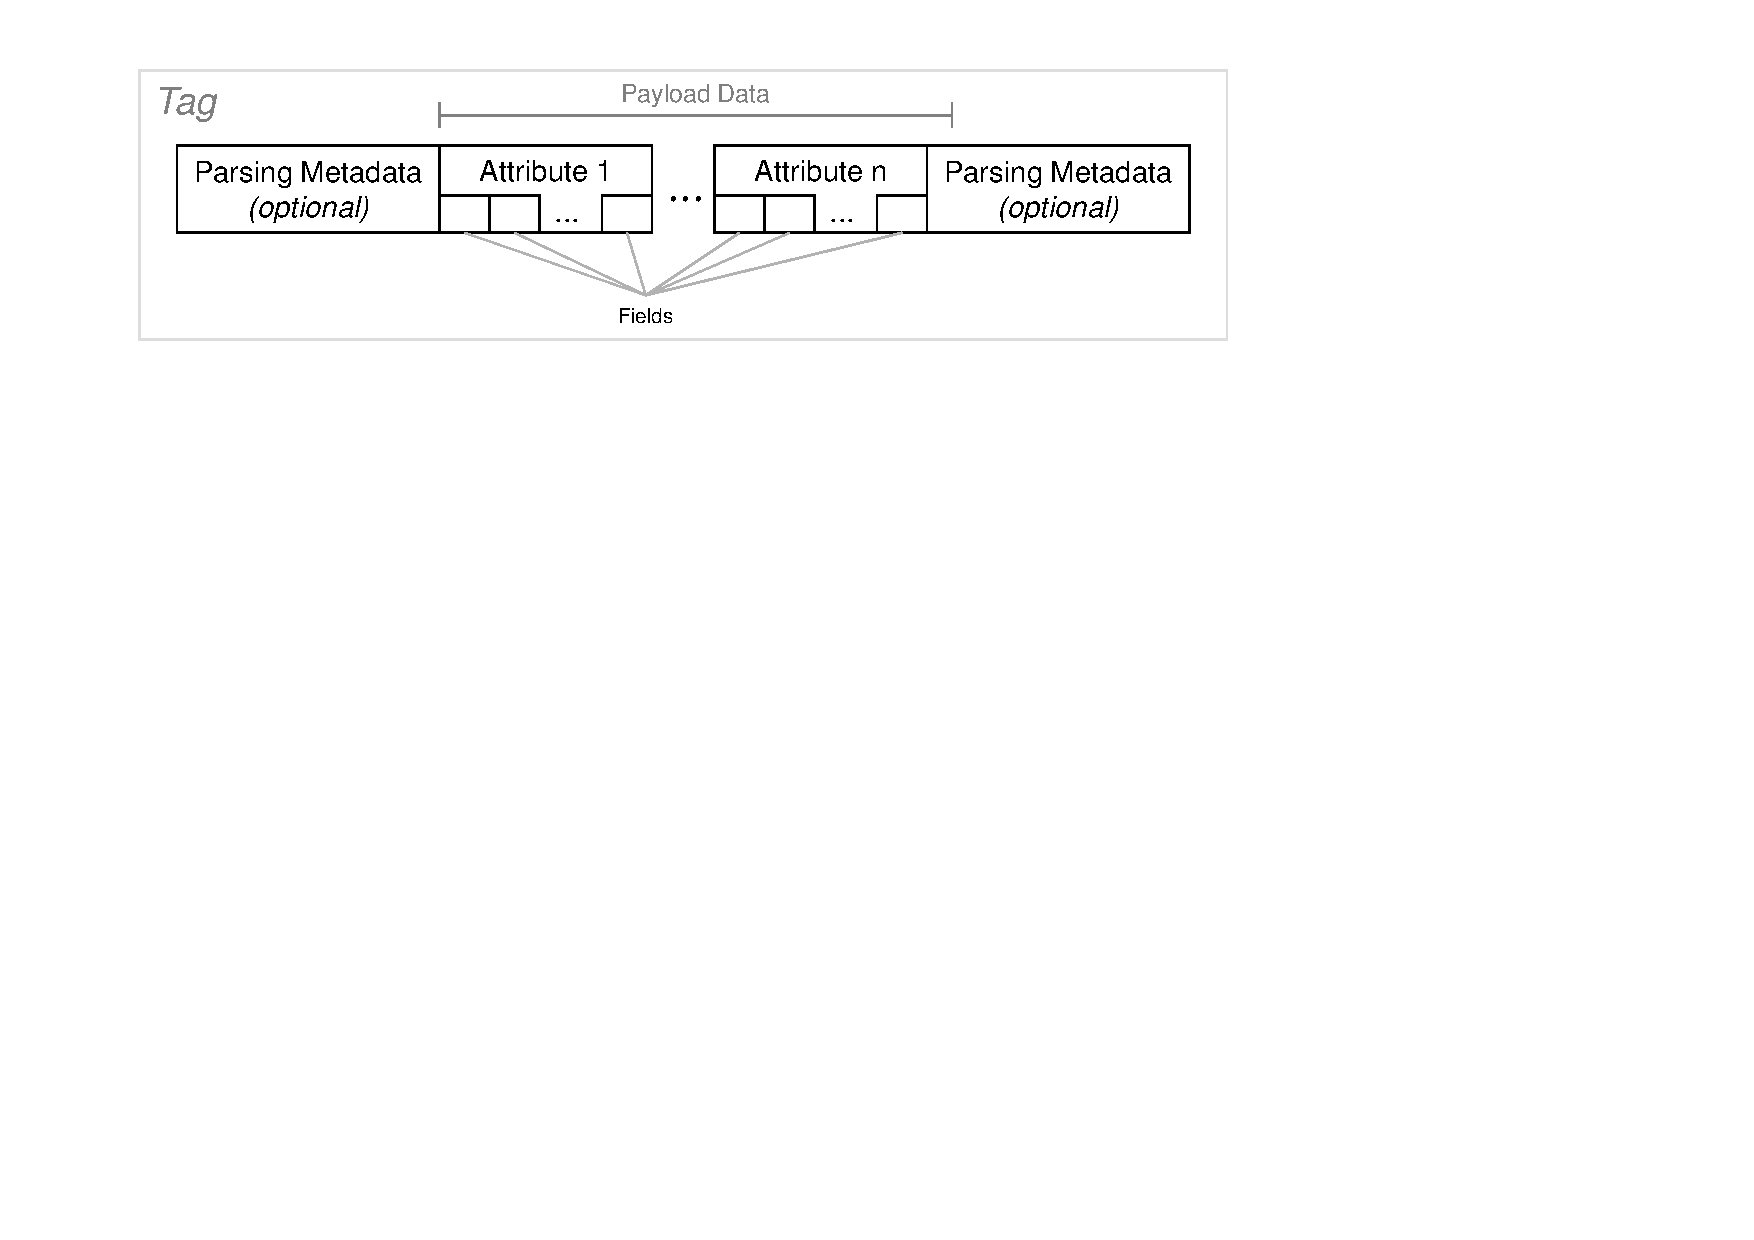
\includegraphics[width=1.00\textwidth]{Figures/Part_I/I_3_TagStructure.pdf}
		\caption{Structure of a \TERMtag{}}
	\label{fig:5_3_SCH_Tag}
\end{figure}

The most important parts of a \TERMtag{} are the \TERMattribute{}s.

%***********************************************************************************************

\subsection{\TERMattribute{}}
\label{sec:Attribute}

An \TERMattribute{} is a part of a \TERMtag{} that contains the valuable metadata information in a key-value manner. Common examples are artist, title, album, composer etc. of a piece of audio. Often, an \TERMattribute{} is also a \TERMcontainer{} in a sense that it has a \TERMheader{}. The \TERMheader{} may help to define the type (artist, title, album) of the \TERMattribute{} as well as the size of the payload. The \TERMpayload{} contains the actual information in an encoded way, e.g. the name of the artist or title of the piece of audio.

Most of the \TERMattribute{}s have a simple main value that can be given. However, there are also more complex \TERMattribute{}s that consists of many values in form of child \TERMdataBlock{}s or \TERMfield{}s.

In each metadata format, an \TERMattribute{} has a specific name, e.g.:
\begin{itemize}
	\item ID3v1, Lyrics3: Field
	\item ID3v2: Frame
	\item APE: Item
	\item Matroska: SimpleTag
	\item VorbisComment: User Comment
\end{itemize}

In \TERMcontainerFormat{}s, the \TERMattribute{}s are often \TERMcontainer{}s defined by the \TERMcontainerFormat{}.

%***********************************************************************************************

\subsection{\TERMfield{}s}
\label{sec:Fields}

A \TERMfield{} is a sequence of bits that together have a specific meaning in a given \TERMdataFormat{}. The \TERMdataFormat{} describes how a specific \TERMdataBlock{} is built up by a specific sequence of \TERMfield{}s. A \TERMfield{} has a range of possible values and
interpretations of these values. Often, one part of the value range is defined as ``reserved'' to ensure a bit of flexibility in extending the data format.

%-----------------------------------------------------------------------------------------------

\subsection{\TERMsubject{}}
\label{sec:Subject}

A \TERMsubject{} represents a thing a \TERMtag{} describes, i.e. a part of a file, a piece of audio, a web resource or even a thing existing in reality. Often, a \TERMtag{} contains metadata for the current \TERMmedium{}, not explicitly referring to a more specific \TERMsubject{}.

%-----------------------------------------------------------------------------------------------

\section{\TERMmedium{}}
\label{sec:Medium}

A medium is the place where data \TERMdataBlock{}s are physically persisted and accessible. This may be a file, a \TERMmediaStream{} or even plain memory.

%###############################################################################################
%###############################################################################################
%
%		File end
%
%###############################################################################################
%###############################################################################################
%===============================================================================================
%		Anforderungen
%===============================================================================================

\chapter{Anforderungen und Ausschl�sse}
\label{sec:Requirements}

Hier werden all expliziten Anforderungen an die Bibliothek \LibName{} in Version \LibVersion{} sowie auch explizite Ausschl�sse dargestellt. Ausschl�sse dienen daf�r, explizit klarzumachen, welche Themen (auf potentiell bliebig lange Zeit) nicht unterst�tzt werden. Davon abzugrenzen sind bereits bekannte (ggf. sogar notwendige) Erweiterungen, die aber nicht in dieser Version verf�gbar sind, sondern absehbar in einer folgenden Version umgesetzt werden sollen. Das sind (potentielle) Features, die auf eine sp�tere Version verschoben worden sind. Diese sind im Abschnitt \SectionLink{sec:FuerSpaeter} beschrieben.

%-----------------------------------------------------------------------------------------------
%		ANF 001
%-----------------------------------------------------------------------------------------------

\section{ANF 001: Metadaten Menschenlesbar lesen und schreiben}
\label{sec:MetadatenLesenUndSchreiben}

Metadaten sollen in \emph{menschenlesbarer Form} gelesen und geschrieben werden k�nnen. D.h. der Anwender der Library wird nicht gen�tigt, bin�re Repr�sentationen der Daten zu erzeugen, um sie schreiben zu k�nnen, bzw. bin�re Daten zu interpretieren. 

\textbf{Begr�ndung:} Dies ist eine generelle Kernfunktionalit�t der Library.

Eine Liste der unterst�tzten Formate findet sich in \SectionLink{sec:Features}.

%-----------------------------------------------------------------------------------------------
%		ANF 002
%-----------------------------------------------------------------------------------------------

\section{ANF 002: Containerformate lesen}
\label{sec:ANF002ContainerformateLesen}

Popul�re bzw. verbreitete Containerformate m�ssen gelesen werden k�nnen.

\textbf{Begr�ndung:} Metadaten sind oft in Containerformaten eingebettet bzw. fest in deren Spezifikation verankert. Zudem m�ssen Container-Segmente erkannt werden k�nnen, um sie zu �berspringen und den eigentlichen Anfang der Metadaten finden zu k�nnen.

%-----------------------------------------------------------------------------------------------
%		ANF 003
%-----------------------------------------------------------------------------------------------

\section{ANF 003: Spezifikation unterst�tzter Metadaten- und Containerformate erf�llen}
\label{sec:ANF003SpezifikationUnterstuetzterMetadatenUndContainerformateErfuellen}

Sofern eine Spezifikation eines unterst�tzten Metadaten- bzw. Containerformates vorliegt, muss diese vollst�ndig unterst�tzt werden. Es muss vollst�ndigen Zugriff auf alle unterst�tzten Features des Datenformates m�glich sein.

\textbf{Begr�ndung:} So wird sichergestellt, dass spezifikationskonforme Metadaten geschrieben werden, die auch von anderen Libraries bzw. Anwendungen wieder gelesen werden k�nnen. Zudem kann der Nutzer der Library alle Features des jeweiligen Formates ausnutzen, ohne wiederum allzu viel Eigenimplementierung leisten zu m�ssen. Dies ist auch eine Differenzierungsm�glichkeit gegen�ber anderen Libraries.

%-----------------------------------------------------------------------------------------------
%		ANF 004
%-----------------------------------------------------------------------------------------------

\section{ANF 004: Zugriff auf alle Rohdaten �ber die Library}
\label{sec:ANF004ZugriffAufAlleRohdatenUeberDieLibrary}

Zus�tzlich zum Zugriff auf menschenlesbare Metadaten (\SectionLink{sec:MetadatenLesenUndSchreiben}) soll es ebenso m�glich sein, alle Rohdaten aub Byteebene zu lesen. Es soll feingranularer Zugriff auf alle Felder der Bin�rdaten m�glich sein.

\textbf{Begr�ndung:} So k�nnen Anwender selbst ein Parsing implementieren, ohne die high-level-Funktionen nutzen zu m�ssen. Sie k�nnen selbst auf Byte- und Bitebene Daten manipulieren und auslesen. Ein Zugriff auf die Bin�rdaten ist m�glich (wenn n�tig), ohne wiederum einen eigenen Umweg gehen zu m�ssen, z.B. durch erneutes Lesen und Parsen der Daten.

%-----------------------------------------------------------------------------------------------
%		ANF 005
%-----------------------------------------------------------------------------------------------

\section{ANF 005: Performance vergleichbar mit anderen Java-Metadaten-Libraries}
\label{sec:ANF005PerformanceVergleichbarMitAnderenJavaMetadatenLibraries}

Die Performance der Library soll gleichwertig oder besser als die anderen Java-Metadaten-Libraries sein. Hierf�r m�ssen die Vergleichslibraries benannt und ein entsprechender Benchmark definiert und durchgef�hrt werden.

\textbf{Begr�ndung:} Die Library soll �hnlich performant wie bestehende L�sungen der idealerweise performanter sein, um hier kein Argument gegen ihren Einsatz zu liefern.

%-----------------------------------------------------------------------------------------------
%		ANF 006
%-----------------------------------------------------------------------------------------------

\section{ANF 006: Fehlererkennung, Fehlertoleranz, Fehlerkorrektur}
\label{sec:ANF006FehlererkennungFehlertoleranzFehlerkorrektur}

Erg�nzend zur \SectionLink{sec:ANF003SpezifikationUnterstuetzterMetadatenUndContainerformateErfuellen} muss die Library aber auch \emph{fehlertolerant} sein, so weit m�glich. D.h. u.a., das Spezifikationsverst��e und fehlerhafte Parsing-Metadaten erkannt werden, und dies - soweit nicht unumg�nglich - nicht zum Abbruch des Parsens mit einem Fehler endet. Verst��e werden protokolliert und wenn m�glich automatisch korrigiert (optional, wenn es der Library-Anwender w�nscht).

\textbf{Begr�ndung:} Altanwendungen oder andere Libraries schreiben Datenformate manchmal nicht 100\% spezifikationskonform. Zudem sind nicht alle Spezifikationen eindeutig oder genau genug, sodass Varianten entstehen k�nnten. Trotz Vorliegen fehlerhafter Daten soll der Anwender der Library in die Lage versetzt werden, Daten dennoch auslesen und ggf. sogar korrigieren zu k�nnen.

%-----------------------------------------------------------------------------------------------
%		ANF 007
%-----------------------------------------------------------------------------------------------

\section{ANF 007: Extensibility for new Metadata and Container Formats}
\label{sec:ANF007ErweiterbarkeitUmNeueMetadatenUndContainerformate}

\LibName{} must be comfortably extensible with new container or metadata formats. As the minimum level, easy extensibility by the library developers must be possible. As the maximum level of extensibility, also end users with programming experience must be able to easily write extensions without too much configuration or boilerplate code.

\textbf{Rationale:} New metadata formats are developed and are available over and over again. The extensibility ensures a longer life time of the library and allows easier maintenance by the library developers. In the maximum level ``Extensibility by end users'', this is a clear differntiation criterion to other libraries that do not offer this level of extensibility.

%-----------------------------------------------------------------------------------------------
%		ANF 008
%-----------------------------------------------------------------------------------------------

\section{ANF 008: Lesen und Schreiben gro�er Datenbl�cke}
\label{sec:ANF009LesenSchreibenGrosse}

\LibName{} muss das Lesen und Schreiben sehr gro�er Datenmengen effizient unterst�tzen, und dabei Mechanismen verwenden, um OutOfMemoryErrors zu vermeiden.

\textbf{Begr�ndung:} Besonders im Video-Bereich k�nnen teilweise gigabyte-gro�e Nutzdaten vorkommen. Die L�nge der Nutztdaten muss korrekt interpretiert werden k�nnen. Wegen \SectionLink{sec:ANF004ZugriffAufAlleRohdatenUeberDieLibrary} muss auch das Lesen und Schreiben der Nutzdaten unterst�tzt werden, ohne dass Speicher knapp wird, d.h. ein etappenweises Lesen und Schreiben o.�. muss m�glich sein. Dies ist auch ein Differenzierungsmerkmal zu anderen Libraries, die dies ggf. gar nicht unterst�tzen k�nnen.

%-----------------------------------------------------------------------------------------------
%		ANF 009
%-----------------------------------------------------------------------------------------------

\section{ANF 009: Selective Format Choice}
\label{sec:ANF010SchreibenInAnderesAusgabemediumUnterst�tzt}

An application using \LibName{} must be able to selectively choose these formats that it wants to support. This is not only necessary for runtime, but also for the library extension packages it wants to use.

\textbf{Rationale:} Audio applications do not need extensions for video or image formats. Applications can minimize the runtime and memory overhead by choosing as few extensions as really needed.

%-----------------------------------------------------------------------------------------------
%		AUS 001
%-----------------------------------------------------------------------------------------------

\section{AUS 001: Lesen aus Media Streams}
\label{sec:AUS009LesenAusStreams}

Ein Lesen von Metadaten oder Containerdaten aus Streams (streaming media) wird nicht explizit unterst�tzt. Es k�nnen im Design M�glichkeiten zur aktiven Unterst�tzung vorgesehen werden, dies ist aber nicht zwingend erforderlich.

\textbf{Begr�ndung:} Kombinierte Anwendungen (Recorder bzw. Player) machen f�r diesen Fall mehr Sinn und sind auch weitgehend verf�gbar. Die zus�tzliche Unterst�tzung f�r Streaming k�nnte das Design verkomplizieren. Es ist aktuell unklar, wie dies umzusetzen w�re.

%-----------------------------------------------------------------------------------------------
%		AUS 002
%-----------------------------------------------------------------------------------------------

\section{AUS 002: Lesen von XML-Metadaten}
\label{sec:AUS010LesenVonXMLMetadaten}

Es gibt auch XML-Metadatenformate. �blicherweise werden diese aber nicht in Multimedia-Daten eingesetzt, da sie sehr ``verbos'' sein k�nnen. Hier sind weiterhin die bin�ren Metadatenformate die Platzhirsche. Die Unterst�tzung von XML wird nicht im Kern der Library vorgesehen.

\textbf{Begr�ndung:} Der Versuch, sowohl bin�re als auch XML-Formate �ber die gleiche API oder gar Implementierung zu unterst�tzen, kann zu einem sehr komplizierten Design f�hren. Java bietet viele sinnvolle Standard-M�glichkeiten zum Parsen und zum Schreiben von XML-Metadaten. Evtl. k�nnten diese in Ausbaustufen in einer Implementierung (hinter der gleichen API-Schnittstelle) in einer sp�teren Ausbaustufe unterst�tzt werden.

%-----------------------------------------------------------------------------------------------
%		AUS 003
%-----------------------------------------------------------------------------------------------

\section{AUS 003: No User Extensions for \LibName{} Media}
\label{sec:AUS01220LesenVonXMLMetadaten}

Extending \LibName{} with new media to support - on top of the out-of-the box supported media - is not supported.

\textbf{Rationale:} The mechanisms available should cover 80 to 90 percent of the use cases. Extensibility by new media might increase the complexity of \LibName{} itself and the extension mechanism in specific, without adding real-world use cases really needing it. It is currently not clear which media beyond streams, byte arrays and files might be candidates for extending \LibName{}. Should new media make sense in future, a new core release can be created to also support media extensions.

%###############################################################################################
%###############################################################################################
%
%		File end
%
%###############################################################################################
%###############################################################################################
%===============================================================================================
%		Reference Examples
%===============================================================================================

\chapter{Reference Examples}
\label{sec:ReferenceExamples}

To proof conformance with the \LibName{} requirements, a set of (mostly) real-life examples for all supported formats is used. The examples are used to illustrate design decisions and also to verify them. In this chapter, these examples are presented for short. The concrete detailed structures of each data format is described in \cite{MetadataCompendium}.

Note that the sizes of the data blocks in the following illustrating example figures do not have any specific meaning.

%-----------------------------------------------------------------------------------------------
%		Example 1: MP3 File with ID3v2.3 and ID3v1.1
%-----------------------------------------------------------------------------------------------

\section{Example 1: MP3 File with ID3v2.3, ID3v1.1 and Lyrics3}
\label{sec:Example1MP3FileWithID3v23AndID3v11}

The following figure shows the first example, an MP3 file with three \TERMtag{}s, ID3v2.3, Lyrics3v2 and ID3v1.1. All are located at the end of the file:

\begin{figure}[H]
	\centering
	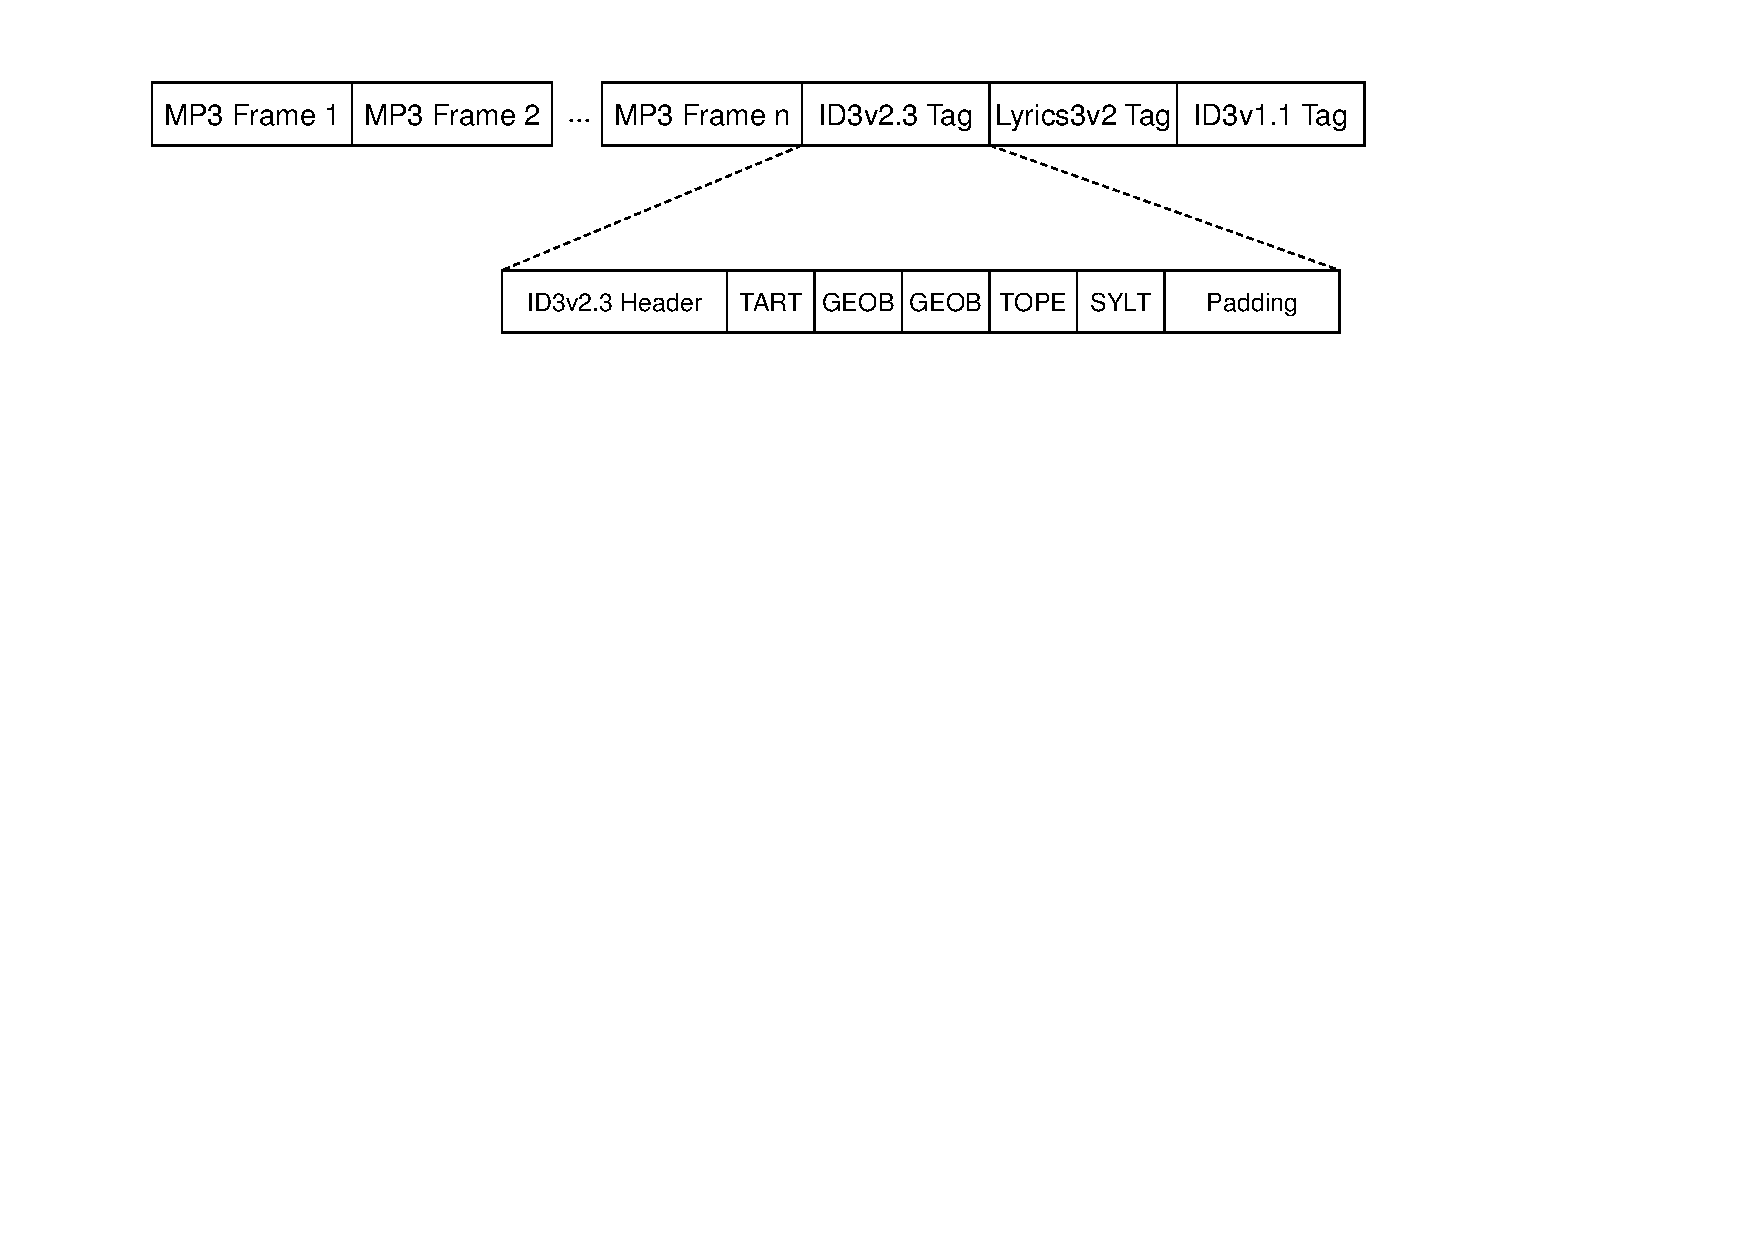
\includegraphics[width=1.00\textwidth]{Figures/Part_I/I_5_Example1.pdf}
	\caption{Example 1: MP3 file with two tags}
	\label{fig:Example1MP3filewithtwotags}
\end{figure}

The ID3v2.3 tag has several frames, including two \texttt{GEOB} frames. Furthermore, it has some padding within. Each of the MP3 frames corresponds to the MPEG-1 elementary stream audio format.

%-----------------------------------------------------------------------------------------------
%		Example 2: MP3 File with two ID3v2.4 Tags
%-----------------------------------------------------------------------------------------------

\section{Example 2: MP3 File with two ID3v2.4 Tags}
\label{sec:Example2MP3FileWithID3v23AndID3v11}

The following figure shows the second example, an MP3 file with two ID3v2.4 \TERMtag{}s, one at the beginning, the other one at the end of the file:

\begin{figure}[H]
	\centering
	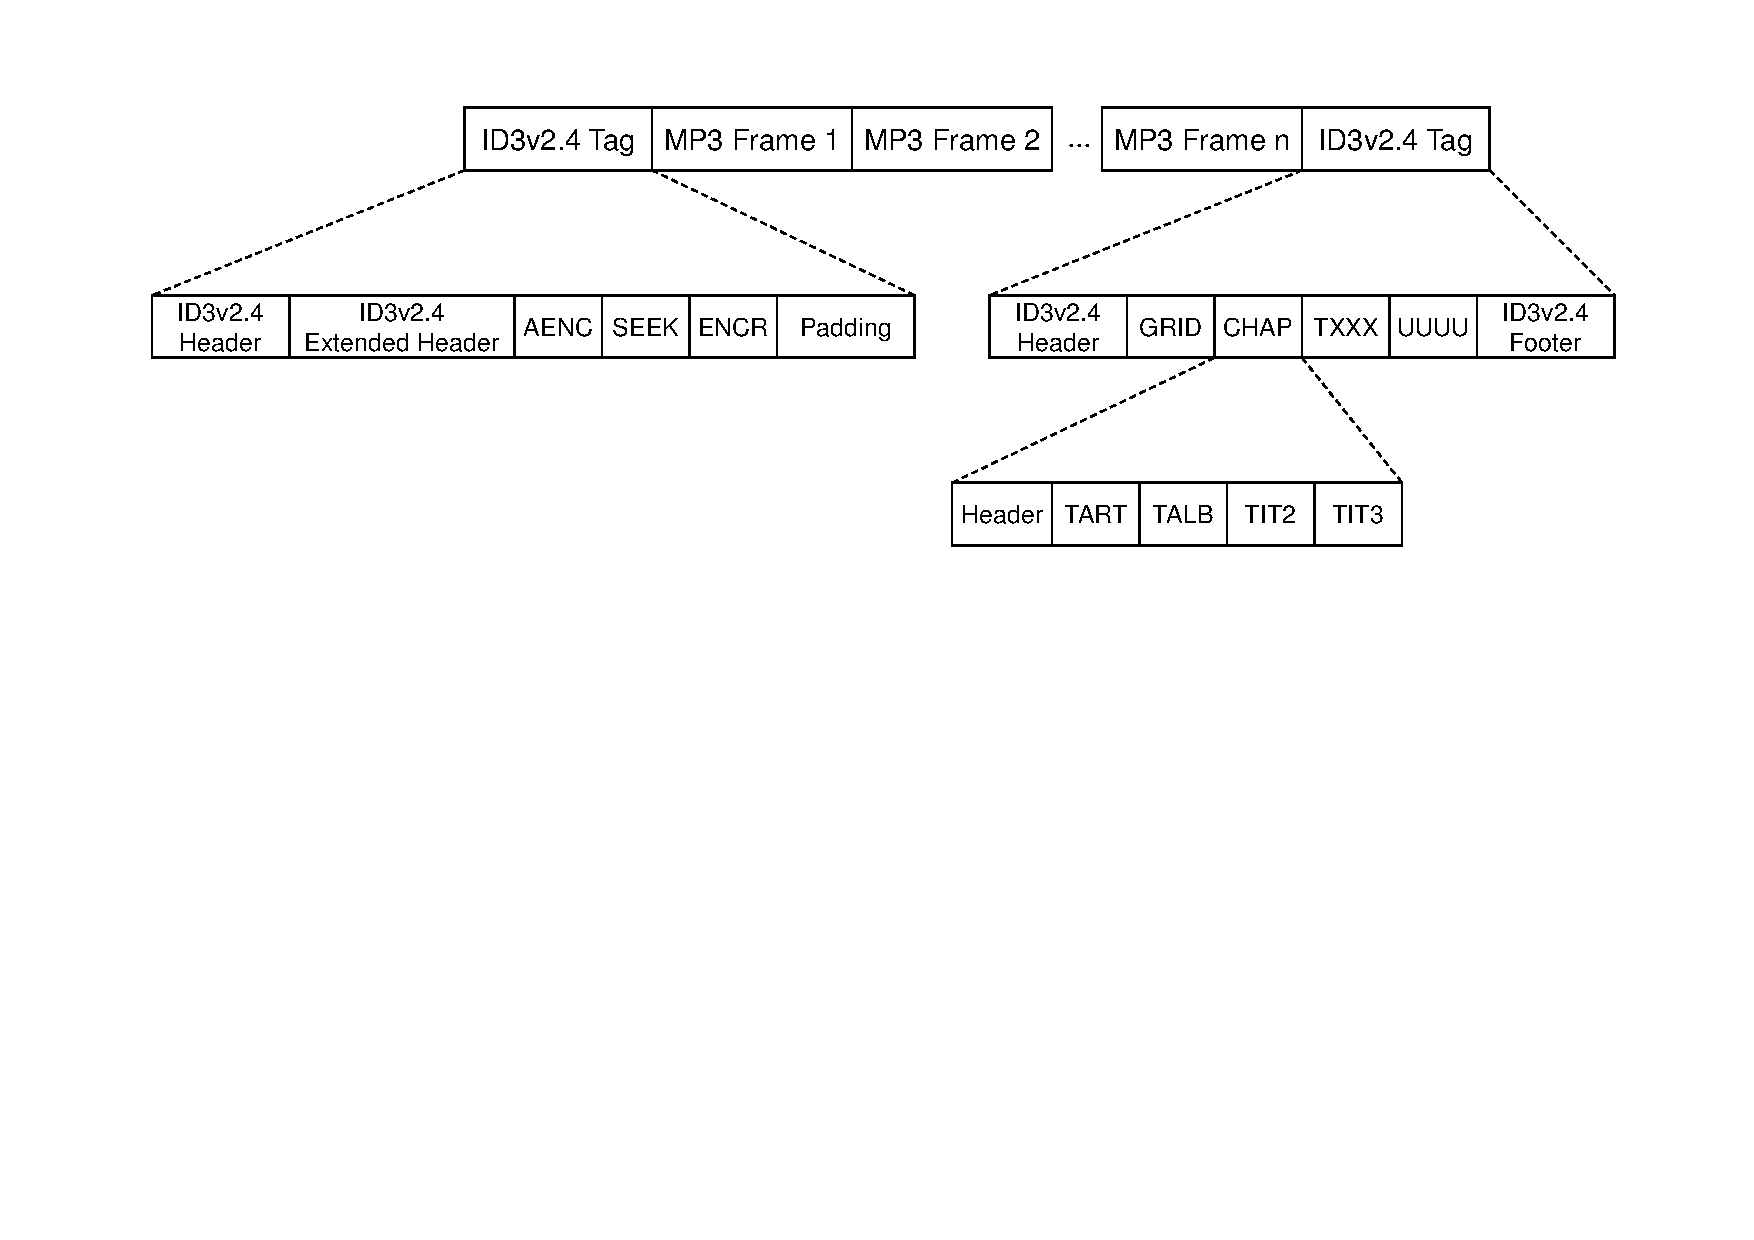
\includegraphics[width=1.00\textwidth]{Figures/Part_I/I_5_Example2.pdf}
	\caption{Example 2: MP3 file with two ID3v2.4 tags}
	\label{fig:Example1MP3filewithtwoID3tags}
\end{figure}

The two ID3v2.4 tags are virtually connected by a \texttt{SEEK} frame. Both have several specialties described in \cite{MetadataCompendium}.

%-----------------------------------------------------------------------------------------------
%		Example 3: MP3 Media Stream with periodic ID3v2.3 Tags
%-----------------------------------------------------------------------------------------------

\section{Example 3: MP3 Media Stream with periodic ID3v2.3 Tags}
\label{sec:Example3MP3FileWithID3v23AndID3v11}

The following figure shows the third example, an MP3 media stream with wildly scattered or periodic ID3v2.3 \TERMtag{}s. The figure shows that start of listening to the stream may also be in the middle of an MP3 block:

\begin{figure}[H]
	\centering
	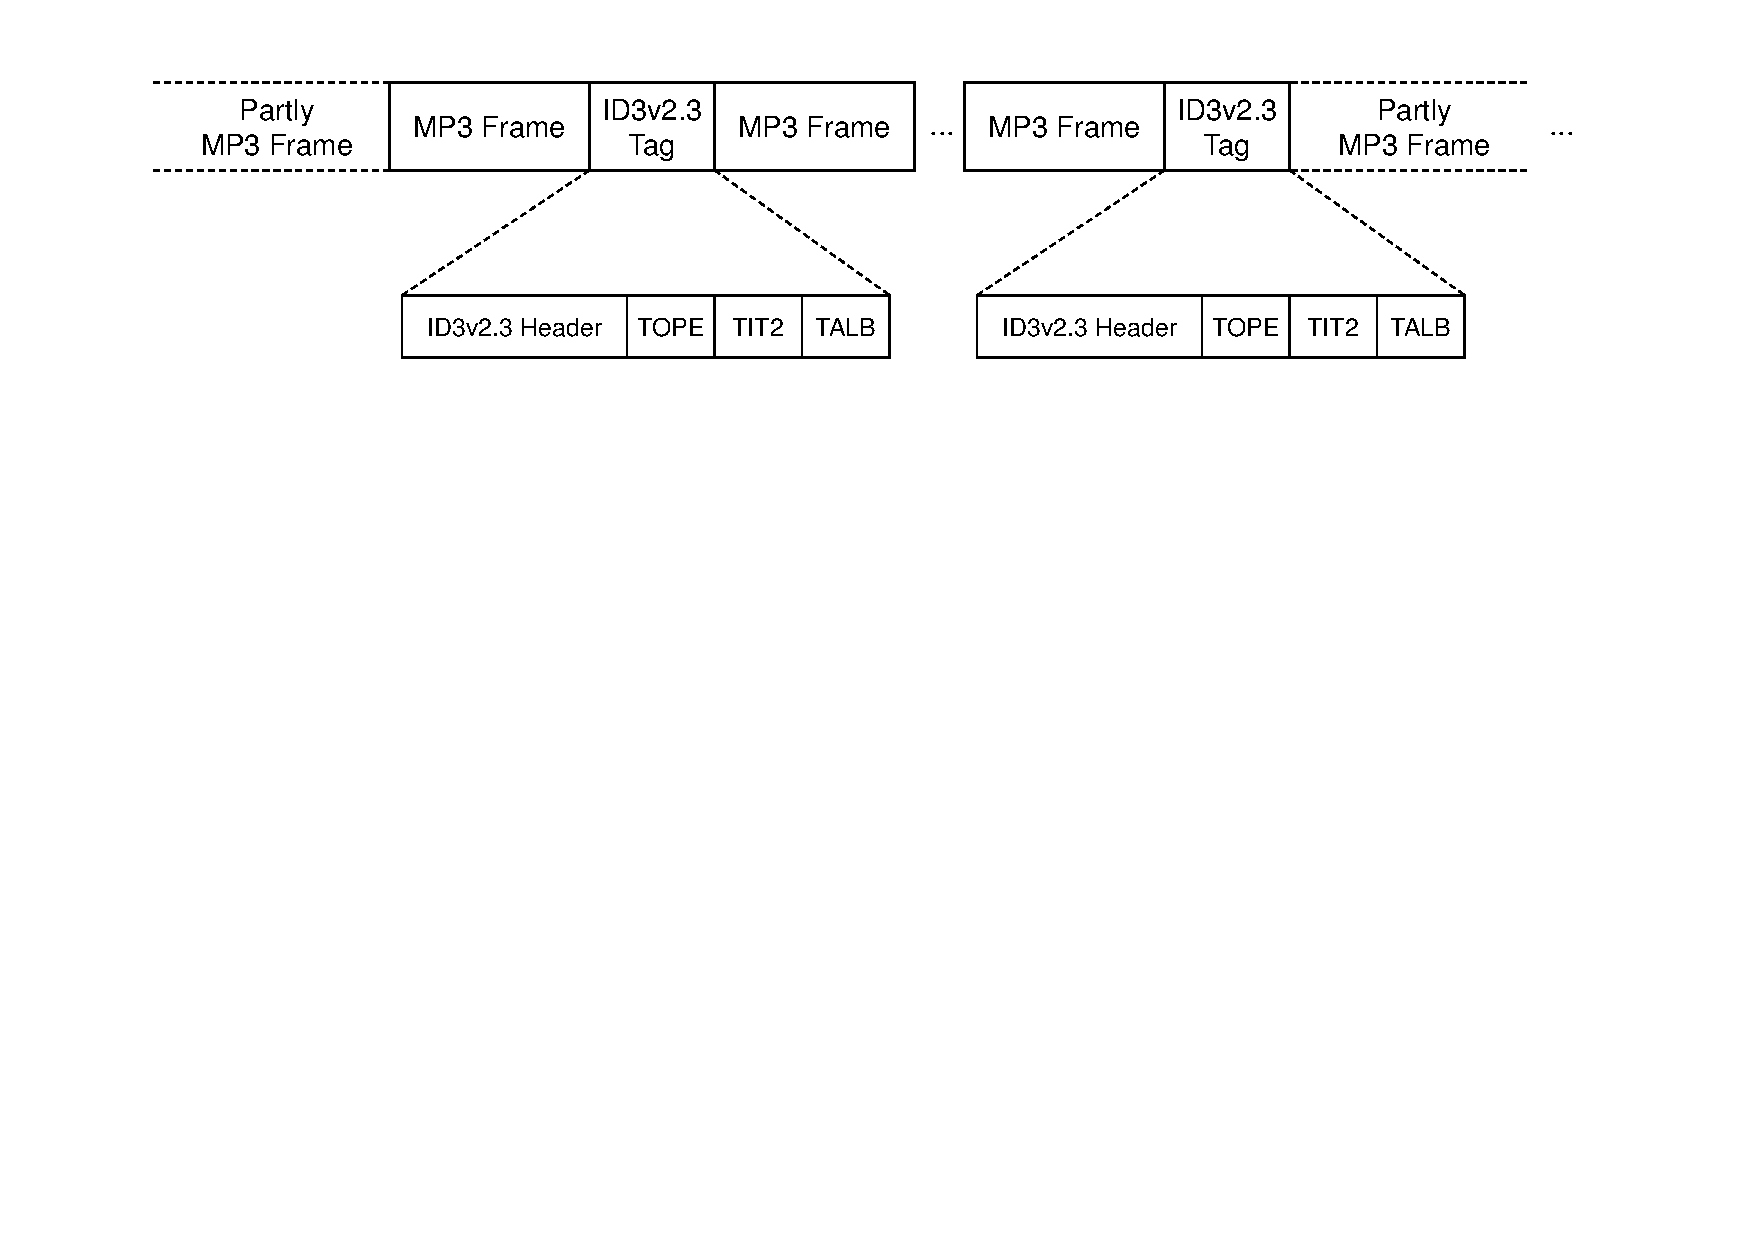
\includegraphics[width=1.00\textwidth]{Figures/Part_I/I_5_Example3.pdf}
	\caption{Example 3: MP3 Media Stream with periodic ID3v2.3 Tags}
	\label{fig:Example3MP3filewithtwoID3tags}
\end{figure}

%-----------------------------------------------------------------------------------------------
%		Example 4: Ogg Bitstream with Theora and VorbisComment
%-----------------------------------------------------------------------------------------------

\section{Example 4: Ogg Bitstream with Theora and VorbisComment}
\label{sec:Example4MP3FileWithID3v23AndID3v11}

The following figure shows the fourth example, an Ogg bitstream that contains Theora payload data with a corresponding vorbis comment:

\begin{figure}[H]
	\centering
	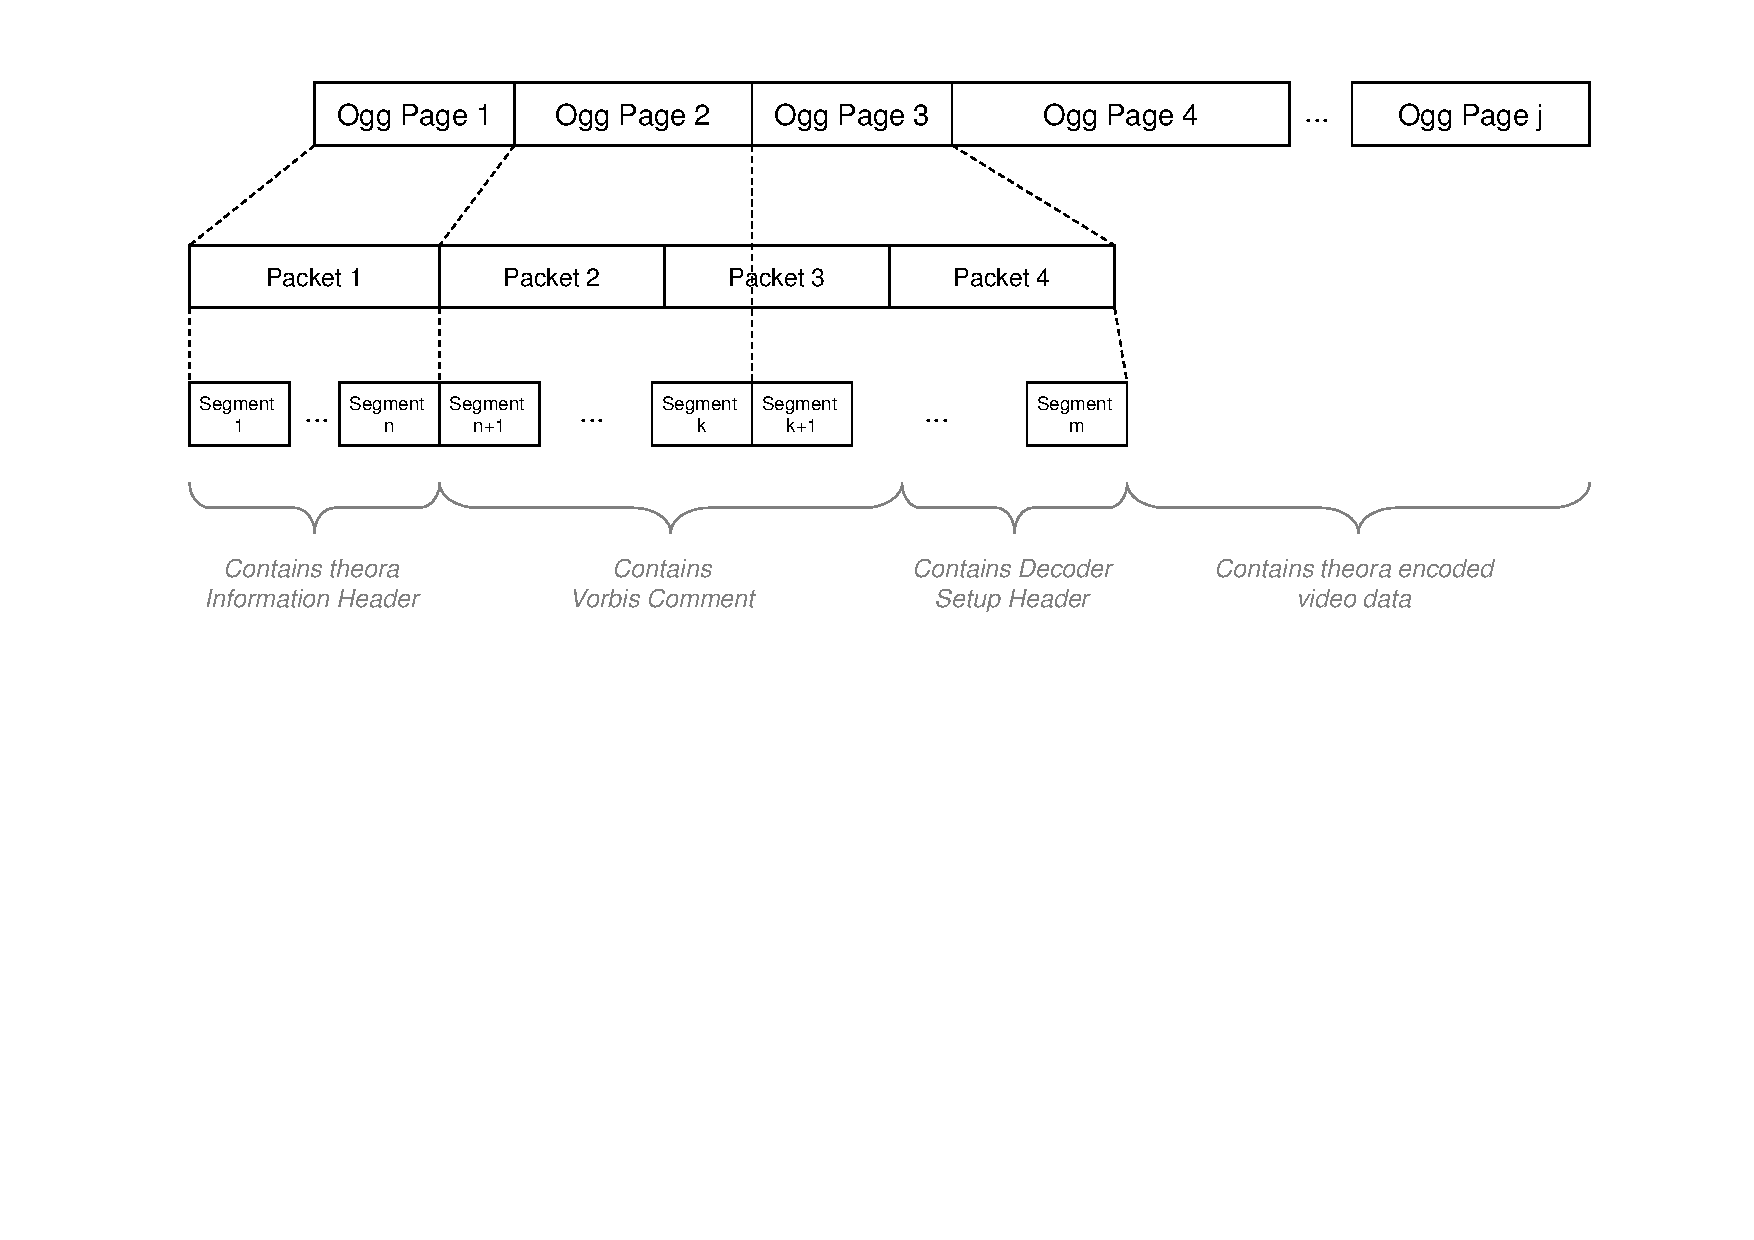
\includegraphics[width=1.00\textwidth]{Figures/Part_I/I_5_Example4.pdf}
	\caption{Example 4: Ogg Bitstream with Theora and VorbisComment}
	\label{fig:Example4MP3filewithtwoID3tags}
\end{figure}

The example is complex on first sight. In an Ogg bitstream, physical and logical structure are not necessarily the same. The physical structure is built by pages, packets and segments, while the logical structure is the structure of the wrapped data. We took theora video data as an example, but its basically arbitrary, as the codec does not really matter. What matters is where the Vorbis Comment, one of the supported data formats, is stored. This unfortunately depends on the embedded codec. In this example, the vorbis comment starts in the second page and spans over two packets. The second of these packets spans over two Ogg pages.

% %-----------------------------------------------------------------------------------------------
% %		Example 5: TIFF RGB image file
% %-----------------------------------------------------------------------------------------------

% \section{Example 5: TIFF RGB image file with Exif IFD}
% \label{sec:Example5MP3FileWithID3v23AndID3v11}

% An example RGB image TIFF file with an Exif IFD is modelled in the following figure:\footnote{The example is based on the figure of \cite{ExifSpec}, page 9.}

% \begin{figure}[H]
% 	\centering
% 	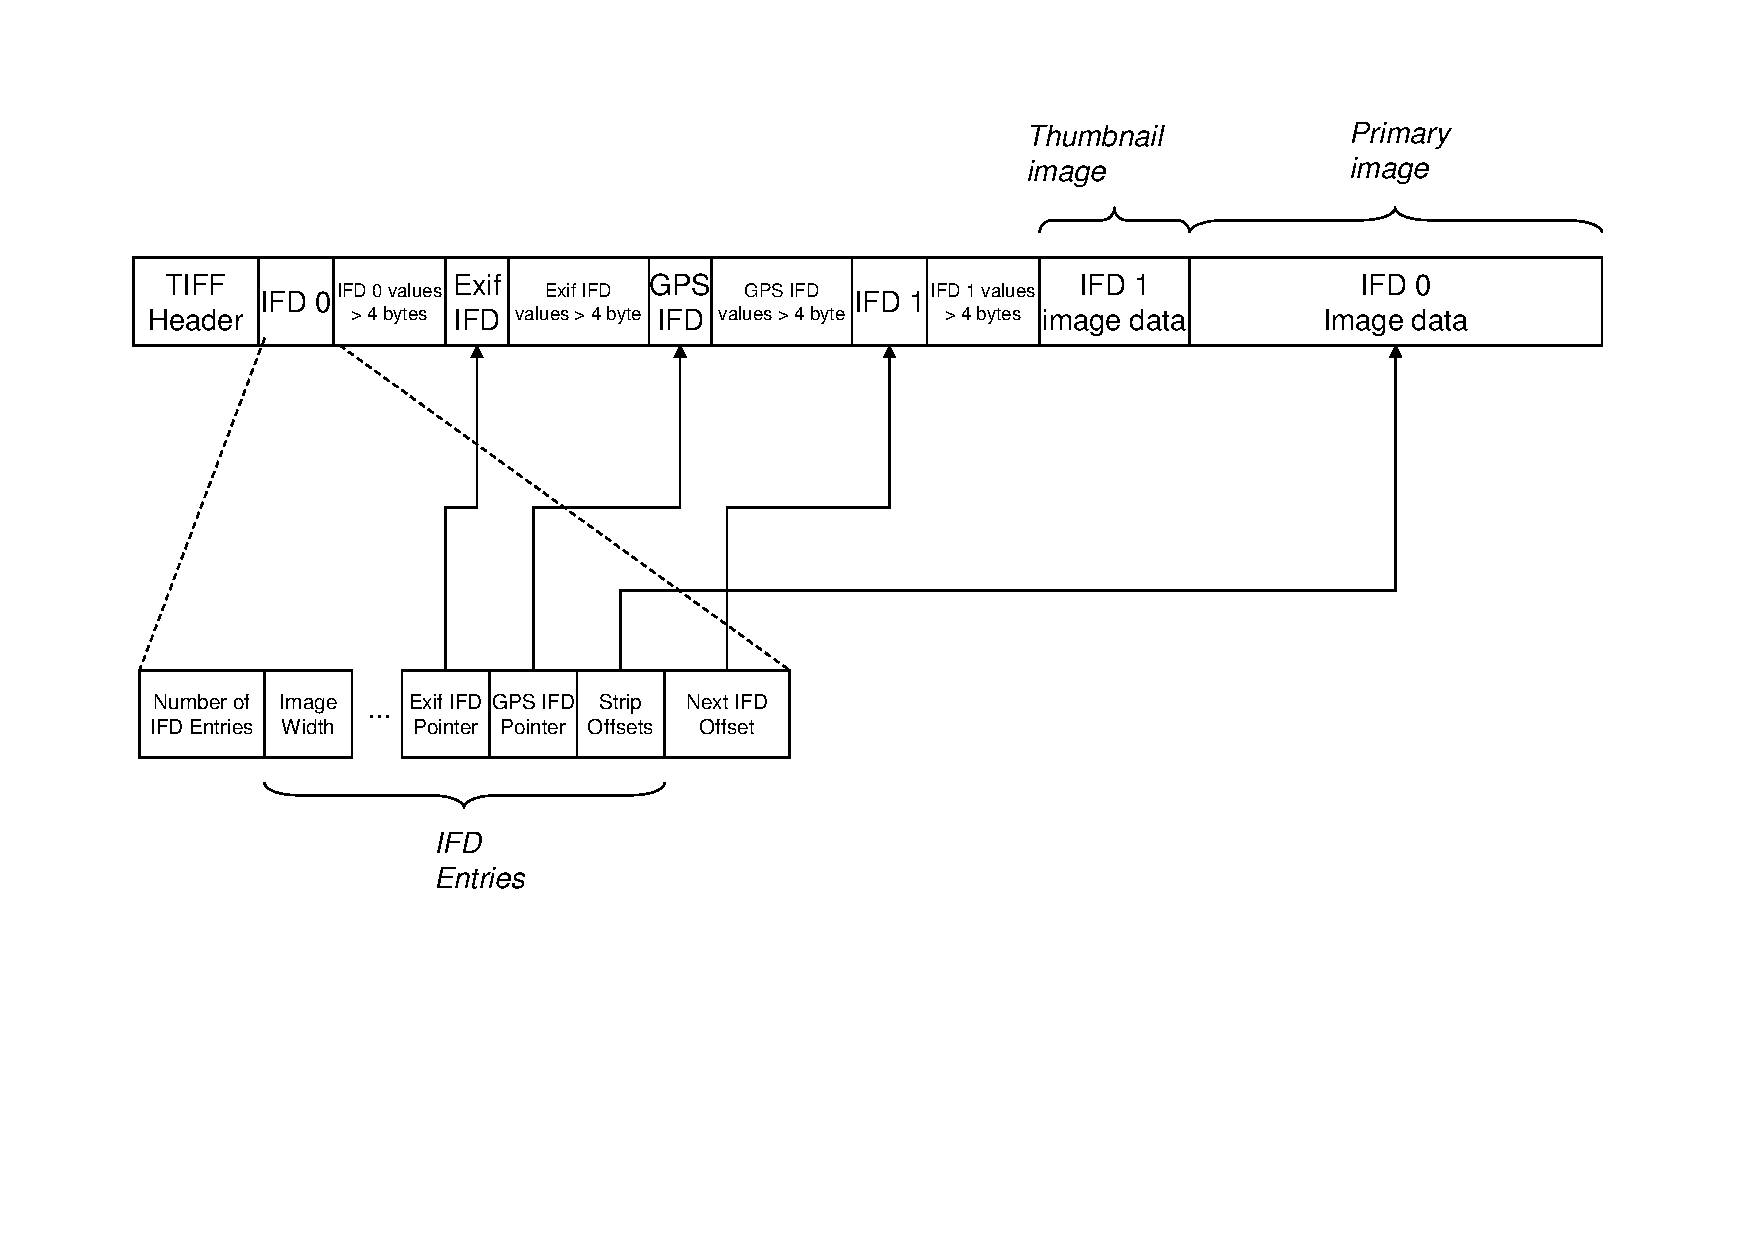
\includegraphics[width=1.00\textwidth]{Figures/Part_I/I_5_Example5.pdf}
% 	\caption{Example 5: TIFF RGB image file with Exif IFD}
% 	\label{fig:Example5MP3filewithtwoID3tags}
% \end{figure}

% Note that Exif is \emph{not a supported format} for \LibName{} currently. However, the presence of an Exif IFD must not be a problem for \LibName{}, of course.

% The example contains two image data parts, in this example stored after each other. The first image part is just a thumbnail image while the second one stores the real image data. The figure shows the pointered structure of the file as IFD fields often point to a byte offset in the file where the actual data is stored.

% %-----------------------------------------------------------------------------------------------
% %		Example 6: RIFF WAVE File
% %-----------------------------------------------------------------------------------------------

% \section{Example 6: RIFF WAVE File}
% \label{sec:Example6MP3FileWithID3v23AndID3v11}

% An example RIFF file with WAVE sound contents is shown in the following figure:

% \begin{figure}[H]
% 	\centering
% 	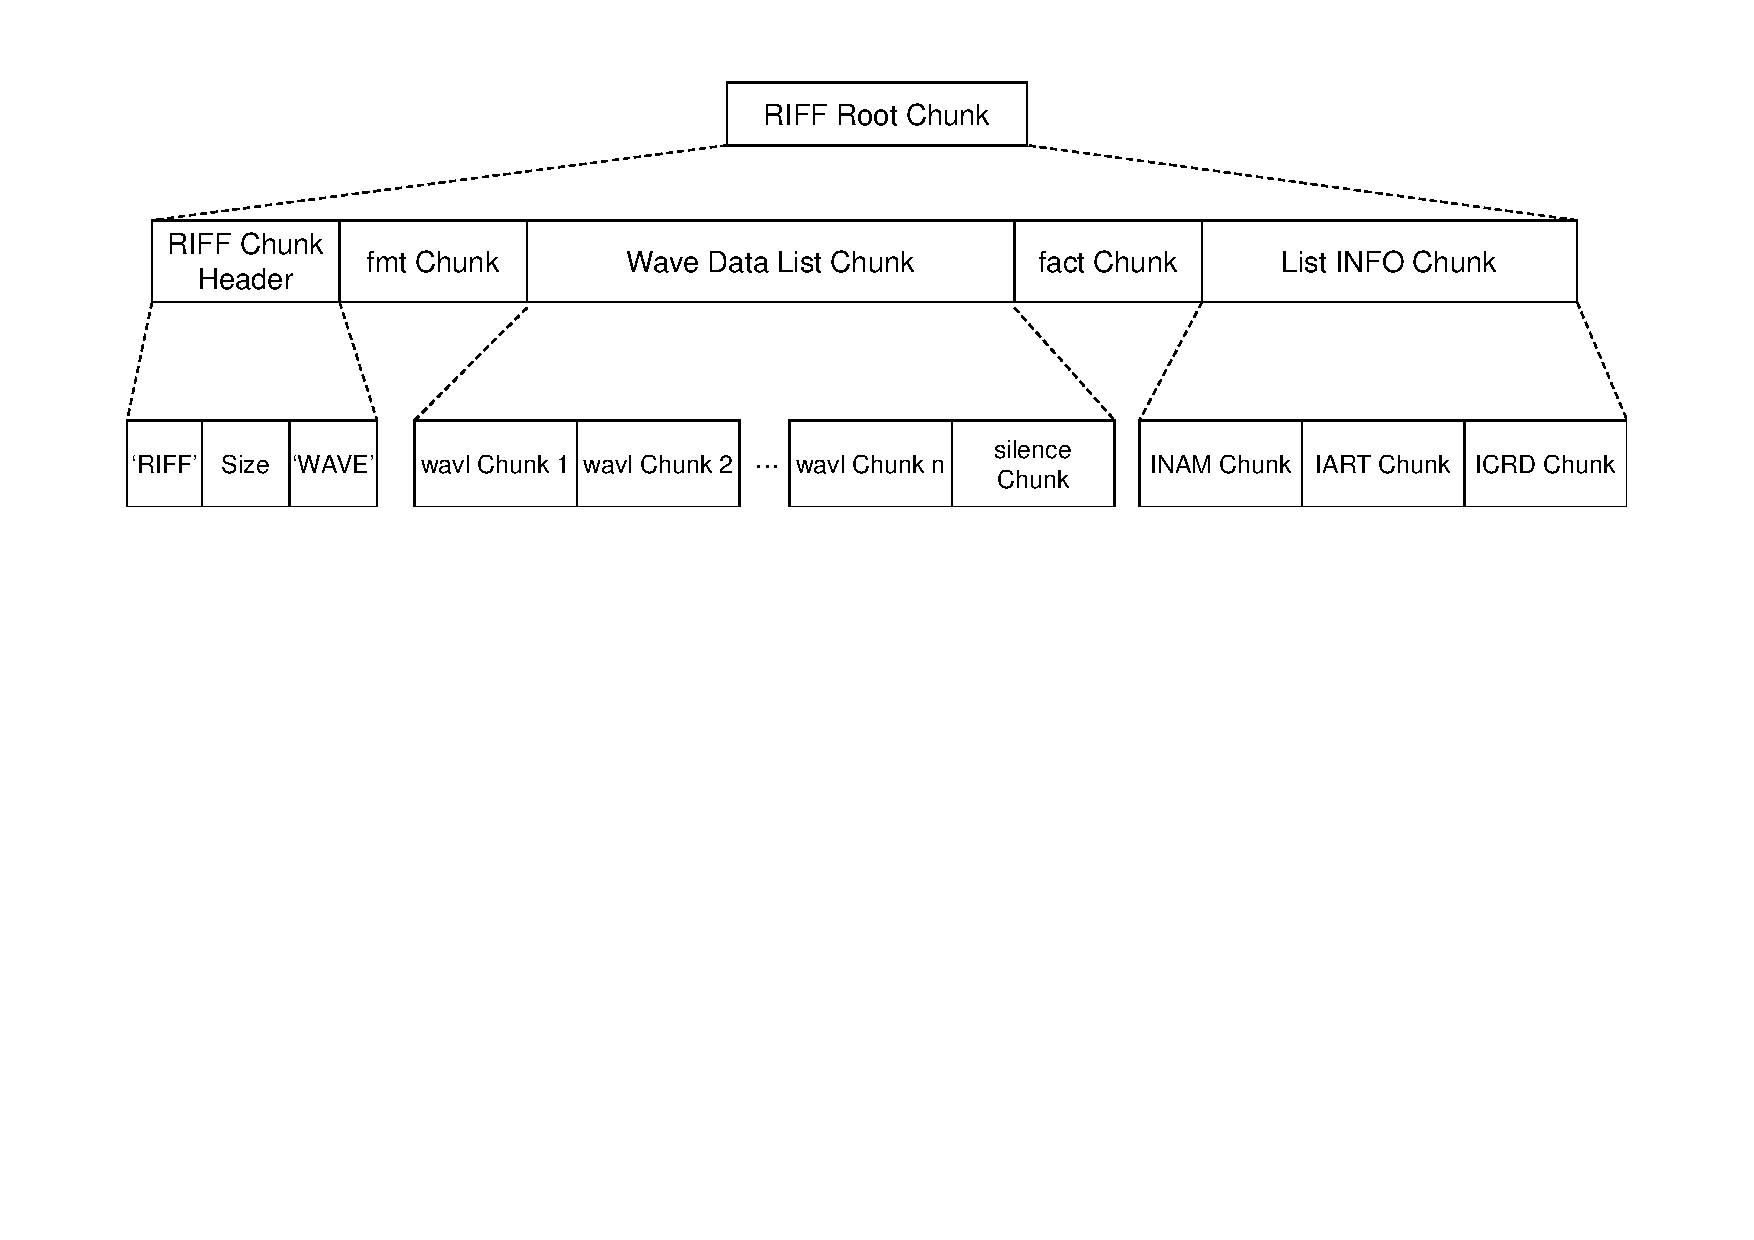
\includegraphics[width=1.00\textwidth]{Figures/Part_I/I_5_Example6.pdf}
% 	\caption{Example 6: RIFF WAVE File}
% 	\label{fig:Example6MP3filewithtwoID3tags}
% \end{figure}

% The top-level root chunk contains a fact chunk, a format chunk, a list of wave data chunks and finally a \texttt{LIST} info chunk in its payload. The \texttt{LIST} info chunk can be considered as \TERMtagBasic{}. It contains \texttt{INAM}, \texttt{IART} and \texttt{ICRD} sub-chunks.

% %-----------------------------------------------------------------------------------------------
% %		Example 7: QuickTime File
% %-----------------------------------------------------------------------------------------------

% \section{Example 7: QuickTime File}
% \label{sec:Example7MP3FileWithID3v23AndID3v11}

% An example QuickTime file is shown in the following figure:

% \begin{figure}[H]
% 	\centering
% 	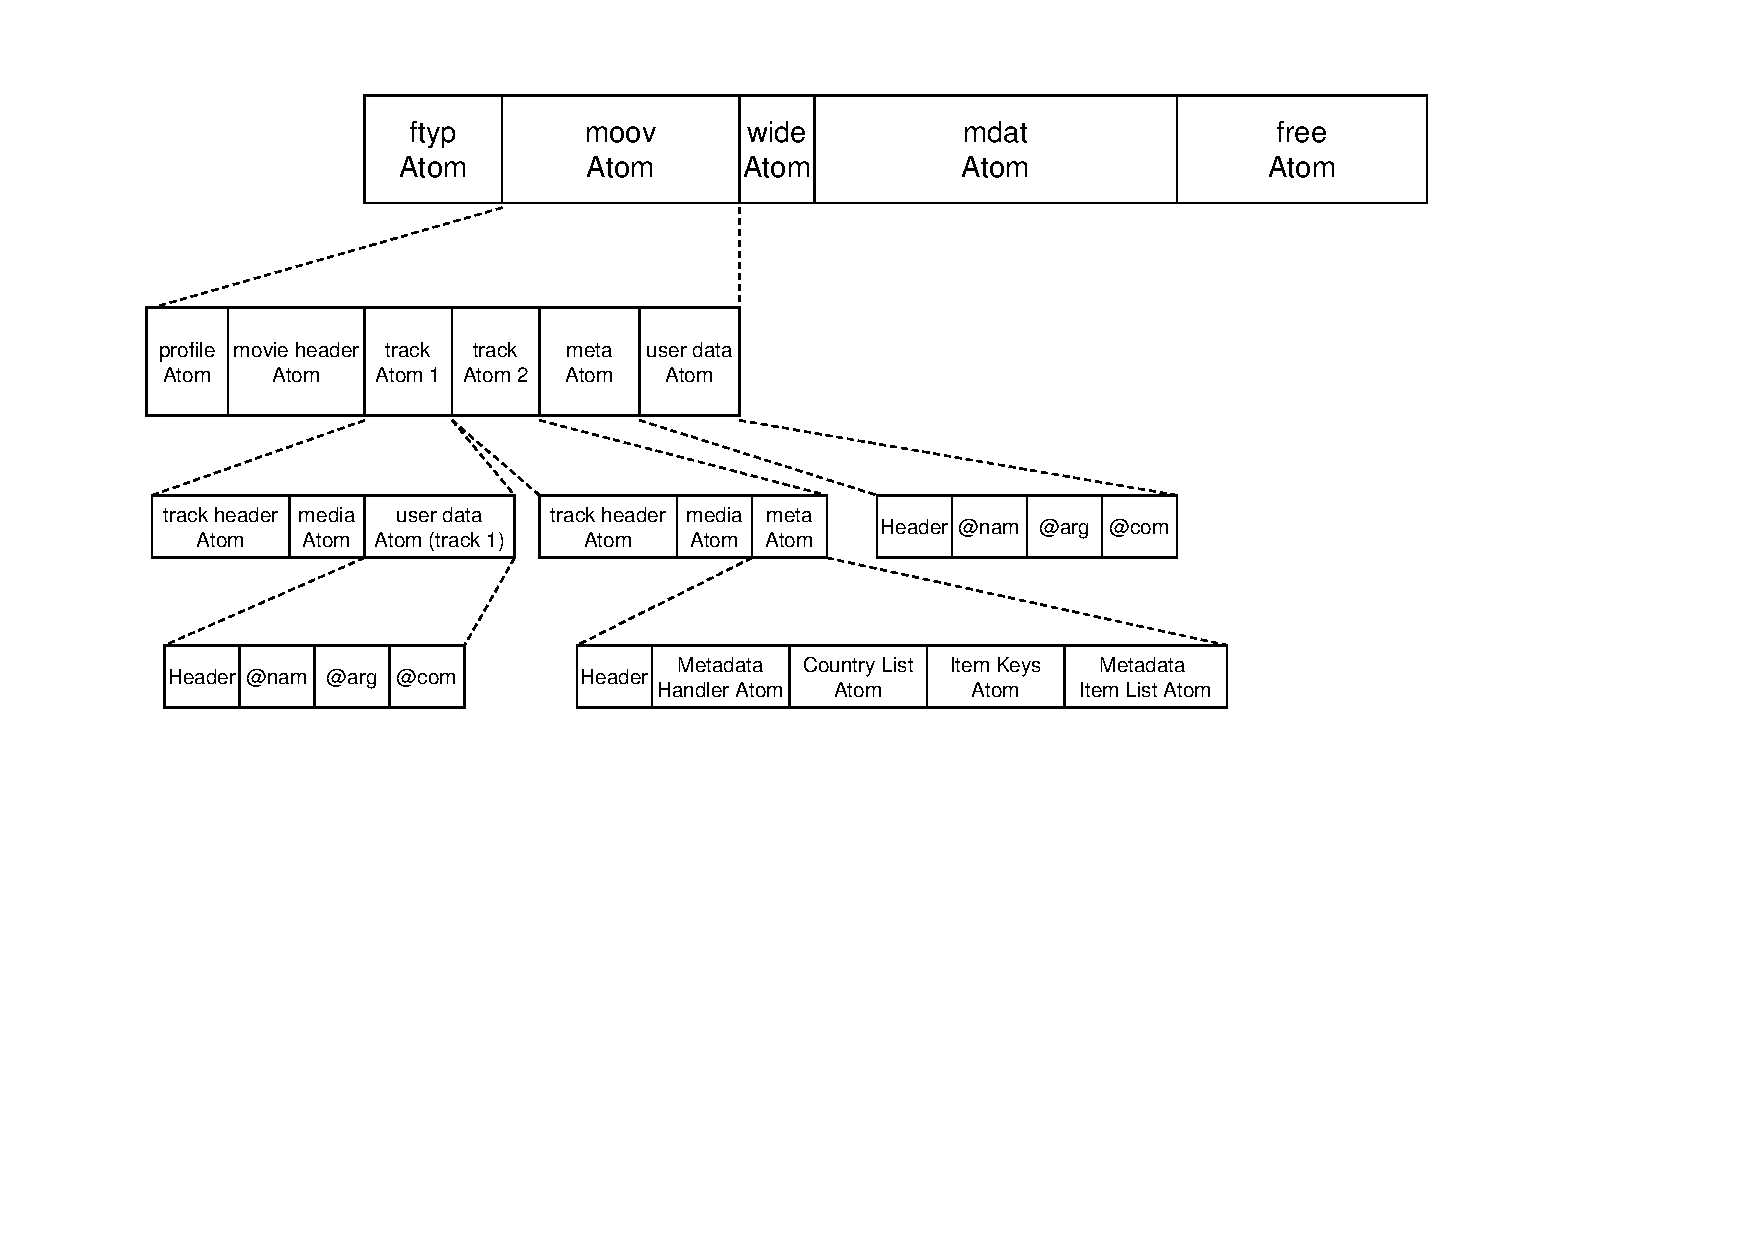
\includegraphics[width=1.00\textwidth]{Figures/Part_I/I_5_Example7.pdf}
% 	\caption{Example 7: QuickTime File}
% 	\label{fig:Example7MP3filewithtwoID3tags}
% \end{figure}

% A QuickTime file can easily get very complex. The example contains the \texttt{ftyp}, \texttt{moov}, \texttt{mdat} and \texttt{free} atoms as top-level atoms. The \texttt{mdat} atom contains the media data and is not further detailed in the example. It is preceded by a wide atom to enable easy extension to a header indicating more than $2^{32}$ bytes media atom size.

% The example defines two tracks in the movie atom. One of these contains a user data atom which contains key-value metadata. The other track contains the QuickTime \texttt{meta} atom also defining metadata, but in a different way.

% The example shows that the \texttt{moov} atom itself additionally contains a \texttt{meta} and user data atom describing the whole file.

% %-----------------------------------------------------------------------------------------------
% %		Example 8: Matroska File
% %-----------------------------------------------------------------------------------------------

% \section{Example 8: Matroska File}
% \label{sec:Example8MP3FileWithID3v23AndID3v11}

% An example Matroska file is shown in the following figure:

% \begin{figure}[H]
% 	\centering
% 	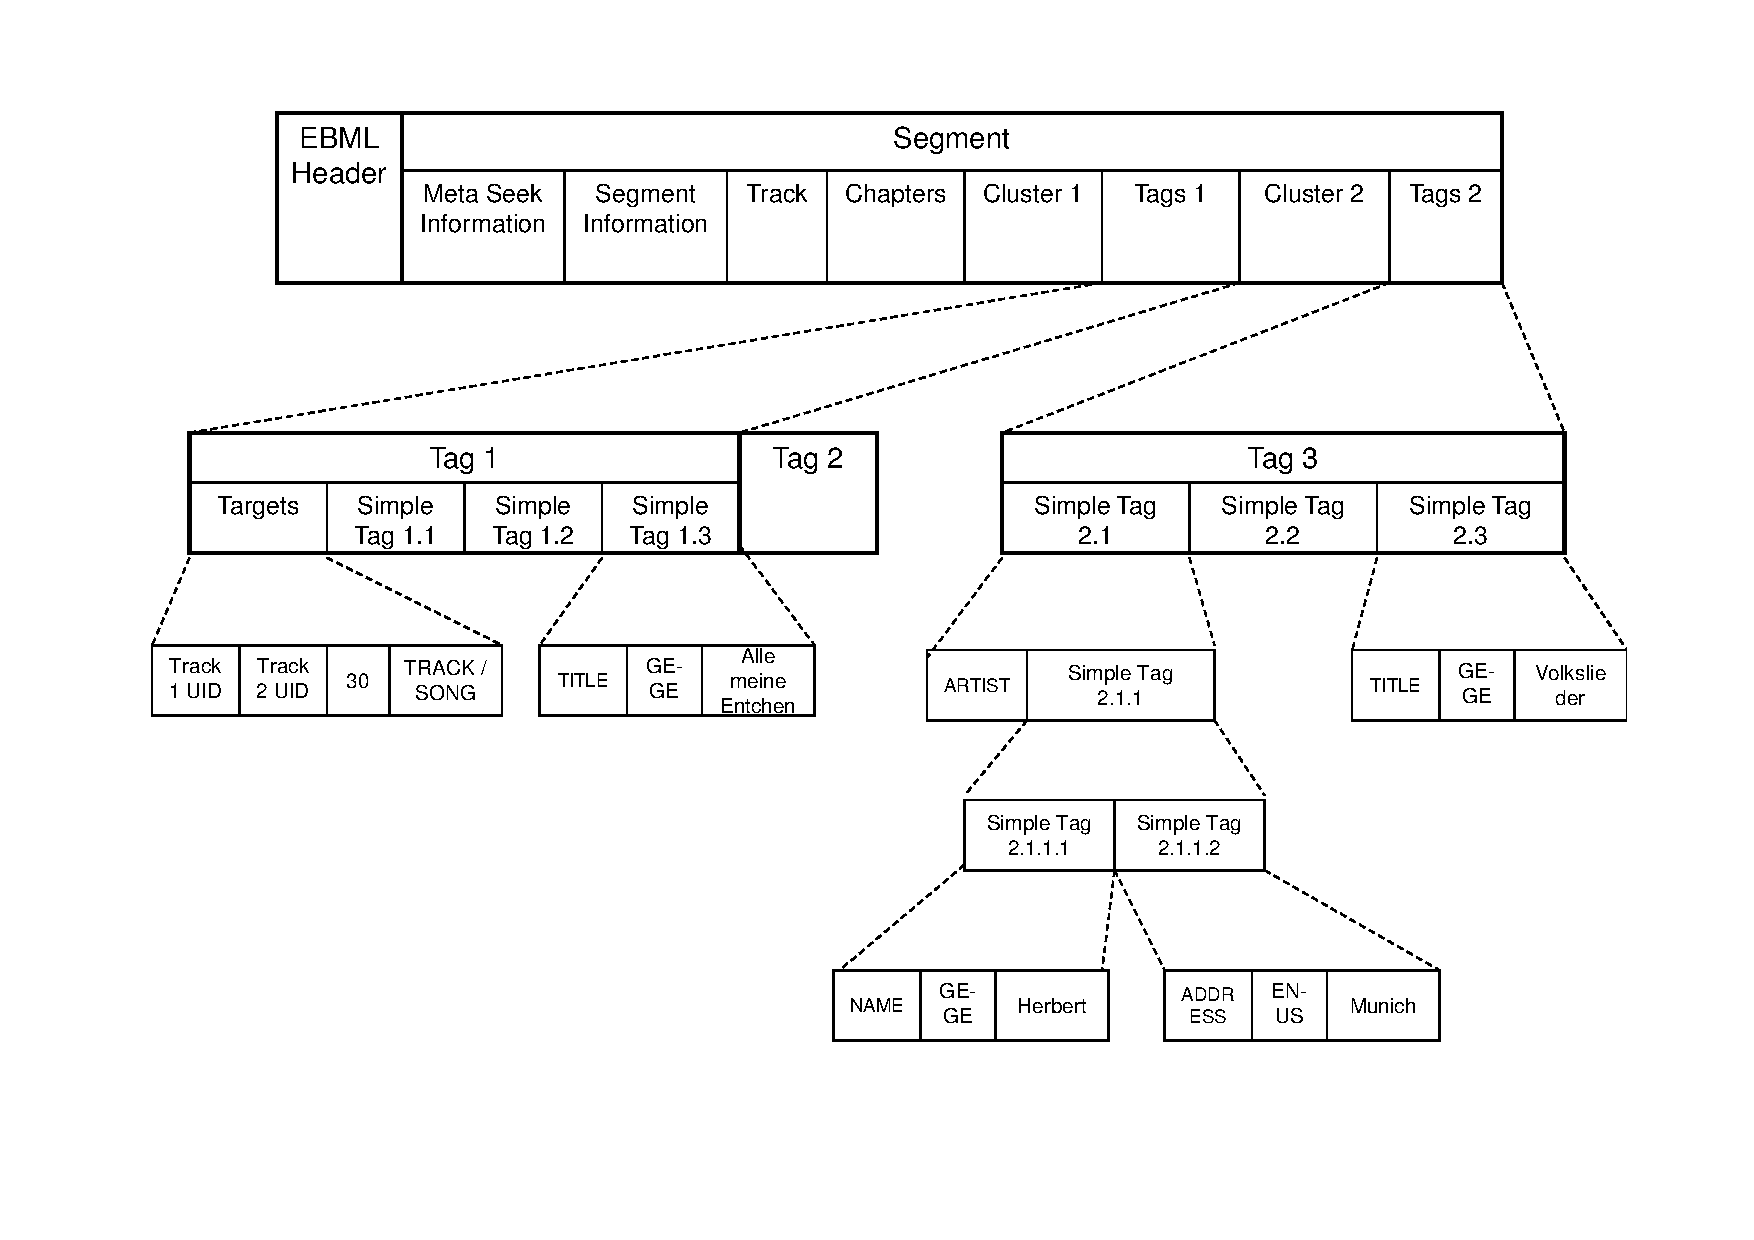
\includegraphics[width=1.00\textwidth]{Figures/Part_I/I_5_Example8.pdf}
% 	\caption{Example 8: Matroska File}
% 	\label{fig:Example8MP3filewithtwoID3tags}
% \end{figure}

% The example has two Cluster elements that store the actual media data. These are not further detailed in the example. The metadata in the example is complex: There are two top-level Tags elements, the first one contains two Tag elements, the second one only a single Tag element. Each of the Tag elements has child SimpleTag elements. The first Tag contains a Targets sub-element that points to two tracks of the file. Tag 3 only contains SimpleTags. However, the first SimpleTag contains nested SimpleTags.

% %-----------------------------------------------------------------------------------------------
% %		Example 9: Arbitrary XML
% %-----------------------------------------------------------------------------------------------

% \section{Example 9: Arbitrary XML}
% \label{sec:Example9MP3FileWithID3v23AndID3v11}

% \LibName{} is required to handle arbitrary XML data, too. The following short file is taken as an example:

% \begin{lstlisting}
% <?xml version="1.0" encoding="UTF-8"?>
% <!DOCTYPE ComponentConfiguration [ 

% <!ELEMENT ComponentDescriptor (Service+)>

% <!ATTLIST id NAME CDATA #REQUIRED>

% ]> 
% <cconf:ComponentConfiguration
% xmlns:cconf="www.easytag.de/XMLSchema_v1_0"
% 	xmlns:xsi="http://www.w3.org/2001/XMLSchema-instance"
% 	xsi:schemaLocation="www.easytag.de/XMLSchema_v1_0 ComponentConfiguration.xsd">
% 	<ComponentDescriptor id="a">
% 		<ProviderPath>bin/</ProviderPath>
% 		<Service>
% 			<Interface>de.je.registry.export.compdummies.a.export.TestInterfaceCompA1</Interface>
% 			<Provider>de.je.registry.compdummies.a.impl.TestImplCompA1</Provider>
% 		</Service>
% 		<Service>
% 			<Interface>de.je.registry.export.compdummies.a.export.TestInterfaceCompA2</Interface>
% 			<Provider>de.je.registry.compdummies.a.impl.TestImplCompA2</Provider>
% 		</Service>
% 	</ComponentDescriptor>
% 	<ComponentDescriptor id="b">
% 		<ProviderPath>bin/</ProviderPath>
% 		<Service>
% 			<Interface>de.je.registry.export.compdummies.b.export.TestInterfaceCompB1</Interface>
% 			<Provider>de.je.registry.compdummies.b.impl.TestImplCompB1</Provider>
% 		</Service>
% 	</ComponentDescriptor>
% 	<ComponentDescriptor id="c">
% 		<ProviderPath>bin/</ProviderPath>
% 		<Service>
% 			<Interface>de.je.registry.export.compdummies.c.export.TestInterfaceCompC1</Interface>
% 			<Provider>de.je.registry.compdummies.c.impl.TestImplCompC1</Provider>
% 		</Service>
% 	</ComponentDescriptor>
% 	<ComponentDescriptor id="d">
% 		<ProviderPath>bin/</ProviderPath>
% 		<Service>
% 			<Interface>de.je.registry.export.compdummies.d.export.XYZ</Interface>
% 			<Provider>de.je.registry.compdummies.d.impl.XYZImpl</Provider>
% 		</Service>
% 	</ComponentDescriptor>
% </cconf:ComponentConfiguration>
% \end{lstlisting}

% The example contains most XML elements: DTD, Elements, attributes, namespaces and of course the XML header.

% %-----------------------------------------------------------------------------------------------
% %		Example 10: Arbitrary XHTML with Meta Elements and RDFa
% %-----------------------------------------------------------------------------------------------

% \section{Example 10: Arbitrary XHTML with Meta Elements and RDFa}
% \label{sec:Example10MP3FileWithID3v23AndID3v11}

% \LibName{} is required to handle arbitrary XHTML data, and especially XHTML meta elements and embedded RDFa. All of this is contained in the following example:

% \begin{lstlisting}
% <?xml version="1.0" encoding="UTF-8"?>
% <!DOCTYPE html
%   PUBLIC "-//W3C//DTD XHTML 1.0 Transitional//EN"
%   "http://www.w3.org/TR/xhtml1/DTD/xhtml1-transitional.dtd">
% <html xmlns="http://www.w3.org/1999/xhtml"
%     version="XHTML+RDFa 1.0"
% 	 xmlns:biblio="http://example.org/"
%     xmlns:dc="http://purl.org/dc/elements/1.1/"
%     xmlns:cal="http://www.w3.org/2002/12/cal/ical#"
%  	 xmlns:foaf="http://xmlns.com/foaf/0.1/"
%     xml:lang="en"
%      profile="http://example.org/profil.html">
%   <head>
%     <title>Books by Marco Pierre White</title>
%     <!-- There is no about attribute here which means the predicate dc:creator with object (i.e. value) "Mark Birbeck" refers to the current document as a subject -->
%     <meta property="dc:creator" content="Mark Birbeck" />
%     <!-- Another example of a predicate that expresses a relationship "foaf:topic" to the specified URI. -->
%     <link rel="foaf:topic" href="http://www.formsPlayer.com/#us" />
% 	 <link rel="foaf:primaryTopic" href="#bbq" />
% 	<title>Beschreibung der Seite</title>
% 	<meta name="Typ" scheme="MIME-Type" content="image/svg+xml">
% 	<meta name="author" content="Anna Lyse">
% 	<meta http-equiv="expires" content="Sat , 01 Dec 2001 00:00:00 GMT">
% 	<meta name="keywords" lang="de" content="Ferien , Griechenland ,
% 		Sonnenschein">
% 	<meta name="keywords" lang="en-us" content="vacation , Greece , sunshine">
% 	<meta name="keywords" lang="en" content="holiday , Greece , sunshine">
% 	<meta name="keywords" lang="fr" content="vacances , Gr&egrave;ce , soleil">
% 	<meta http-equiv="content-type" content="text/html; charset=ISO-8859-1">
% 	<meta http-equiv="Content-Script-Type" content="text/javascript">

% 	<meta http-equiv="PICS-Label" content='(PICS-1.1 "http://www.gcf.org/v2.5"
% 		labels on "1994.11.05T08:15-0500"
% 		unti l "1995.12.31T23:59-0000"
% 		for "http://w3c.org/PICS/Overview.html"
% 		ratings ( suds 0.5 density 0 color/hue 1) ) '>
%   </head>
%   <body>
%     I think White's book
%     <!-- Here comes the first subject embedded in a span element. It refers to a specific datatype using typeof. It is described with the predicate dc:title whose object (i.e. value) is
%     the contents of the span element. -->
%     '<span about="urn:ISBN:0091808189" typeof="biblio:book"
%            property="dc:title">
%       Canteen Cuisine
%     </span>'
%     is well worth getting since although it's quite advanced stuff, he
%     makes it pretty easy to follow. You might also like
%     <!-- The second subject whose dc:description is given. -->
%     <span about="urn:ISBN:1596913614" typeof="biblio:book"
%           property="dc:description">
%       White's autobiography
%     </span>.
%     <!-- Another subject -->
%     <p about="#bbq" typeof="cal:Vevent">
%       I'm holding
%       <span property="cal:summary">
%         one last summer barbecue
%       </span>,
%       on
%       <!-- Here the object is not the content of the span attribute but the value of the "content" attribute -->
%       <span property="cal:dtstart" content="2007-09-16T16:00:00-05:00"
%             datatype="xsd:dateTime">
%         September 16th at 4pm
%       </span>.
%     </p>
% </body>
% </html>
% \end{lstlisting}

% The example is not real but constructed from various sources. It contains as much different elements as possible:
% \begin{itemize}
% 	\item Some meta elements with a @name attribute
% 	\item Some meta elements with a @http-equiv attribute
% 	\item A meta element containing PICS metadata. PICS is not directly supported in \Lib{}. However, the generic meta elements must be parsed correctly, no matter what they contain.
% 	\item Some meta elements using specific namespaces or profiles
% 	\item RDFa metadata
% \end{itemize}

% %-----------------------------------------------------------------------------------------------
% %		Example 11: An RDF/XML File
% %-----------------------------------------------------------------------------------------------

% \section{Example 11: An RDF/XML File}
% \label{sec:Example11MP3FileWithID3v23AndID3v11}

% \begin{lstlisting}
% <?xml version="1.0" encoding="UTF-8"?>
% <rdf:RDF xmlns:rdf="http://www.w3.org/1999/02/22-rdf-syntax-ns#"
%          xmlns:pcv="http://prismstandard.org/namespaces/pcv/1.0/"
%          xmlns:dc="http://purl.org/dc/elements/1.1/"
%          xml:base="http://travel.example.com/"
%          xmlns:s="http://example.org/students/vocab#"
%          xmlns:exterms="http://www.example.org/terms/">

%   <rdf:Description rdf:about="/2000/08/Corfu.jpg">
%     <dc:identifier rdf:resource="/content/2357845" />
%     <dc:creator>
%       <pcv:Descriptor rdf:about="/emp3845">
%         <pcv:label>John Peterson</pcv:label>
%       </pcv:Descriptor>
%     </dc:creator>
%     <dc:coverage>
%       <pcv:Descriptor
%           rdf:about="http://prismstandard.org/vocabs/ISO-3166/GR">
%         <pcv:label xml:lang="en">Greece</pcv:label>
%         <pcv:label xml:lang="fr">Grece</pcv:label>
%       </pcv:Descriptor>
%     </dc:coverage>
%   </rdf:Description>

%   <rdf:Description rdf:about="/2000/08/Corfu.jpg">
%     <dc:identifier rdf:resource="/content/2357845" />
%     <dc:creator>
%     	Michael
%     </dc:creator>
%   </rdf:Description>
  
%    <rdf:Description rdf:about="http://example.org/courses/6.001">
%       <s:students rdf:parseType="Collection">
%          <rdf:Description rdf:about="http://example.org/students/Amy"/>
%          <rdf:Description rdf:about="http://example.org/students/Mohamed"/>
%          <rdf:Description rdf:about="http://example.org/students/Johann"/>
%       </s:students>
%    </rdf:Description>

%   <rdf:Description rdf:about="http://www.example.com/2002/04/products#item10245">
%      <exterms:weight rdf:parseType="Resource">
%        <rdf:value rdf:datatype="&xsd;decimal">2.4</rdf:value>
%        <exterms:units rdf:resource="http://www.example.org/units/kilograms"/>
%      </exterms:weight>
%   </rdf:Description>

% </rdf:RDF>
% \end{lstlisting}

% The example contains several rdf:Description elements, even two referring to the same subject. We also have applications of the rdf:parseType, rdf:datatype and rdf:resource attributes. There are also some nested descriptions.

% %-----------------------------------------------------------------------------------------------
% %		Example 12: An XMP File
% %-----------------------------------------------------------------------------------------------

% \section{Example 12: An XMP File}
% \label{sec:Example12MP3FileWithID3v23AndID3v11}

% The following listing shows the XMP reference example:

% \begin{lstlisting}
% <?xpacket begin='?' id='W5M0MpCehiHzreSzNTczkc9d'?>
% <x:xmpmeta xmlns:x='adobe:ns:meta/' x:xmptk='XMPTk 2.8'>

% <rdf:RDF 
% 	xmlns:rdf='http://www.w3.org/1999/02/22-rdf-syntax-ns#' 
% 	xmlns:iX='http://ns.adobe.com/iX/1.0/'>

% 	<rdf:Description about=''
% 		xmlns:xmp='http://ns.adobe.com/xap/1.0/' 
% 		xmp:Author='Jane Doe'
% 		xmp:BaseURL='http://mydoc'
% 		xmp:CreateDate='2001-08-13T10:42:24Z'
% 		xmp:CreatorTool='Microsoft Visual C++ for Windows'
% 		xmp:Format='text/xml'
% 		xmp:MetadataDate='2001-08-13T10:42:24Z'
% 		xmp:ModifyDate='2001-08-13T11:02:13Z'
% 		xmp:Nickname='sample'>
    
% 		<xmp:Advisory>
% 			<rdf:Bag>    
%  				<rdf:li>http://purl.org/dc/elements/1.1/ format</rdf:li>
% 				<rdf:li>http://ns.adobe.com/xap/1.0/xap/g/ NumberOfColors</rdf:li>
% 				<rdf:li>http://ns.adobe.com/xap/1.0/xap/g/img/ Resolution/stRes:units</rdf:li>
% 			</rdf:Bag>
% 		</xmp:Advisory>
  
% 		<xmp:Authors>  
% 			<rdf:Seq>
% 				<rdf:li>Jane Doe</rdf:li>
% 				<rdf:li>John Doe</rdf:li>
% 				<rdf:li>Jack Doe</rdf:li>
% 			</rdf:Seq>
% 		</xmp:Authors>
% 		<xmp:Description>
% 			<rdf:Alt>
% 				<rdf:li xml:lang='en'>This document is a sample XML file</rdf:li>
% 				<rdf:li xml:lang='fr'>Ce document est un fichier d`exemple XML</rdf:li>
% 				<rdf:li xml:lang='de'>Dieses Dokument ist eine XML Beispieldatei</rdf:li>
% 			</rdf:Alt>
% 		</xmp:Description>
  
% 		<xmp:Keywords>
% 			<rdf:Bag>
% 				<rdf:li>XMP</rdf:li>
% 				<rdf:li>Core</rdf:li>
% 				<rdf:li>Schema</rdf:li>
% 				<rdf:li>sample</rdf:li>
% 			</rdf:Bag>
% 		</xmp:Keywords>
% 		<xmp:Locale>
% 			<rdf:Bag>
% 				<rdf:li>en</rdf:li>
% 				<rdf:li>fr</rdf:li>
% 				<rdf:li>de</rdf:li>
% 			</rdf:Bag>
% 		</xmp:Locale>
  
% 		<xmp:Title>
% 			<rdf:Alt>
% 				<rdf:li xml:lang='en'>XMP Core Schema Example</rdf:li>
% 				<rdf:li xml:lang='fr'>XMP Core Schema Exemple</rdf:li>
% 				<rdf:li xml:lang='de'>XMP Core Schema Beispiel</rdf:li>
% 			</rdf:Alt>
% 		</xmp:Title>
  
% 	</rdf:Description>

% </rdf:RDF>

% </x:xmpmeta>
% <?xpacket end='r'?>

% </top_level_element>
% \end{lstlisting}

%###############################################################################################
%###############################################################################################
%
%		File end
%
%###############################################################################################
%###############################################################################################

%###############################################################################################
%###############################################################################################
%
%		File end
%
%###############################################################################################
%###############################################################################################

%===============================================================================================
%		Part 2: Architektur
%===============================================================================================

\part{Architektur}
\label{sec:Architeture}

In this part, the high-level structure of \LibName{} is defined. This is done in two refinement levels and an additional perspective:
\begin{itemize}
	\item The technical architecture shows the technical environment and parts of \LibName{}
	\item The functional architecture shows and describes the functional components of \LibName{}
	\item The development view shows the structure of the \LibName{} development artifacts
	\item The deployment view shows the structure of the \LibName{} deployment artifacts
\end{itemize}

%===============================================================================================
%		General Design Decisions
%===============================================================================================

\chapter{Allgemeine Designentscheidungen}
\label{sec:GeneralDesignDecisions}

In diesem Kapitel werden allgemeine Designentscheidungen getroffen, die einen unumkehrbaren Einfluss auf die Architektur der Gesamt-Library haben. Sie definieren die Rahmenbedingungen f�r die Library, und dienen als Basis zur Definition ihrer technischen und vorallem fachlichen Architektur. Sie bilden auch generell und �bergreifend die Basis zur Erf�llung der Anforderungen, haben daher noch keinen Bezug zu einer spezifischen Anforderung.

Die Erf�llung der spezifischen Anforderungen wird durch die detaillierten Designentscheidungen erm�glicht, die im Kapitel \SectionLink{sec:FunctionalArchitectureChap} und im Teil \SectionLink{sec:Design} definiert sind.

%-----------------------------------------------------------------------------------------------
%		Design Decision: Java SE 8
%-----------------------------------------------------------------------------------------------

\section{Verwendung von Java}
\label{sec:VerwendungVonJava}

\DD{dd:001}
{% Titel
	\LibName{} basiert auf Java SE 8%
}
{% Kurzbeschreibung
	\LibName{} wird basierend auf dem ``latest update'' von Java SE 8 entwickelt. Ein Umstieg auf neuere Java-Versionen wird im Rahmen des Lebenszyklus der Library wiederholt in Erw�gung gezogen.
}
{% Begr�ndung
Java als Programmiersprache ist etabliert und weit verbreitet sowie plattformunabh�ngig. Prinzipiell ist der Portierungsaufwand zu anderen  Betriebssystemen, Java ME sowie Java f�r Smartphones (z.B. Android) damit weitaus geringer als bei Verwendung von beispielsweise C/C++. Da der Autor langj�hrige Erfahrung mit Java hat, stellt deren Verwendung eine h�chstm�gliche Produktivit�t sicher. Die Konkurrenzlibraries im Java-Umfeld sind �berschaubar. Die aktuell (Stand 15. M�rz 2016) neueste Version Java 8 wird ganz klar deshalb genutzt, weil die neuesten verf�gbaren Features von Sprache und Library genutzt werden sollen. Java 7 hingegen wird ab voraussichtlich April 2015 von Oracle nicht mehr mit �ffentlichen Updates versorft, Support ist aber weiterhin einkaufbar. Somit kann es sein, dass �ffentliche Fixes f�r bekannte Bugs nicht mehr f�r Java 7 erscheinen werden.
}
{% Nachteile
Anwendungen, die auf Java 7 oder �lter basieren, werden von \LibName{} nicht mehr unterst�tzt. Das tr�fe dann insbesondere auf Java-EE-Anwendungen zu, die vielfach noch auf so innovative Produkte wie Websphere 8.0 (oder �lter!) aufsetzen.
}

%-----------------------------------------------------------------------------------------------
%		Design Decision: keine Dritt-Libraries
%-----------------------------------------------------------------------------------------------

\section{Verwendung anderer Libraries}
\label{sec:VerwendungAndLib}

\DD{dd:002}
{% Titel
	\LibName{} setzt so wenig wie m�glich Dritt-Libraries ein
}
{% Kurzbeschreibung
	\LibName{} setzt weitestgehend allein auf die Libraries von Java SE auf. Es werden - im produktiven Code - keine Abh�ngigkeiten zu dritten Libraries genutzt.
}
{% Begr�ndung
Zus�tzliche Abh�ngigkeiten k�nnen zu Mehraufw�nden bei der Verwaltung (Build, Deployment, Versionsmanagement) f�hren. Letztlich ist \LibName{} dann auch von der Lizenzierung, vom Release- und Bug-Management und den ``Launen'' der Library-Entwickler abh�ngig, was hiermit vermieden wird. Zudem wird die Anwendung insgesamt leichtgewichtiger, sowohl zur Laufzeit als auch im Hinblick auf die Auslieferungsgr��e.
}
{% Nachteile
Evtl. h�herer Entwicklungsaufwand, weil das Rad ab und an ``neu erfunden'' wird.
}

%-----------------------------------------------------------------------------------------------
%		Design Decision: komponentenbasiert
%-----------------------------------------------------------------------------------------------

\section{Komponentenbasierte Library}
\label{sec:KomponentenbasierteLibrary}

\DD{dd:003}
{% Titel
	\LibName{} ist komponentenbasiert
}
{% Kurzbeschreibung
	\LibName{} besteht aus sogenannten Komponenten (Definition siehe n�chsten Abschnitt), die sich gegenseitig nur �ber klar definierte Schnittstellen verwenden.
}
{% Begr�ndung
Die Untergliederung in Komponenten erm�glicht es, die Komplexit�t der Library �ber ihren gesamten Lebenszyklus hinweg besser zu beherrschen. Durch eine sinnvolle Komponentengliederung wird eine klare Aufgabentrennung, Entkopplung und eine bessere Erweiterbarkeit sichergestellt. �nderungen an einer Implementierung einer Komponente haben ein deutlich geringeres Risiko, sich auf weite Teile der Library auszuwirken, sondern werden lokal auf die Komponentenimplementierung beschr�nkt bleiben.
}
{% Nachteile
Ggf. etwas mehr overhead und mehr Komplexit�t, da Mechanismen zur Entkopplung eingesetzt werden m�ssen.
}

%-----------------------------------------------------------------------------------------------

\subsection{Definition des Komponentenbegriffs}
\label{sec:ComponentTermDefinition}

Eine \emph{Komponente} in \LibName{} ist \emph{eine abgeschlossene Software-Einheit mit klar definierter Aufgabe}. Sie bietet \emph{Services} an, die �ber eine klar \emph{definierte Schnittstelle} genutzt werden k�nnen. Diese Services werden sowohl von den Anwendern der Library als auch von anderen Komponenten der Library genutzt. Eine Komponente hat ggf. \emph{Datenhoheit} �ber bestimmte Daten, d.h. nur die Komponente selbst darf diese Daten lesen und modifizieren. Andere Komponenten m�ssen diese spezielle Komponente nutzen, um diese Daten zu verwenden. 

Die folgende Abbildung zeigt schmeatisch eine \LibName{} Komponente:

\begin{figure}[H]
	\centering
	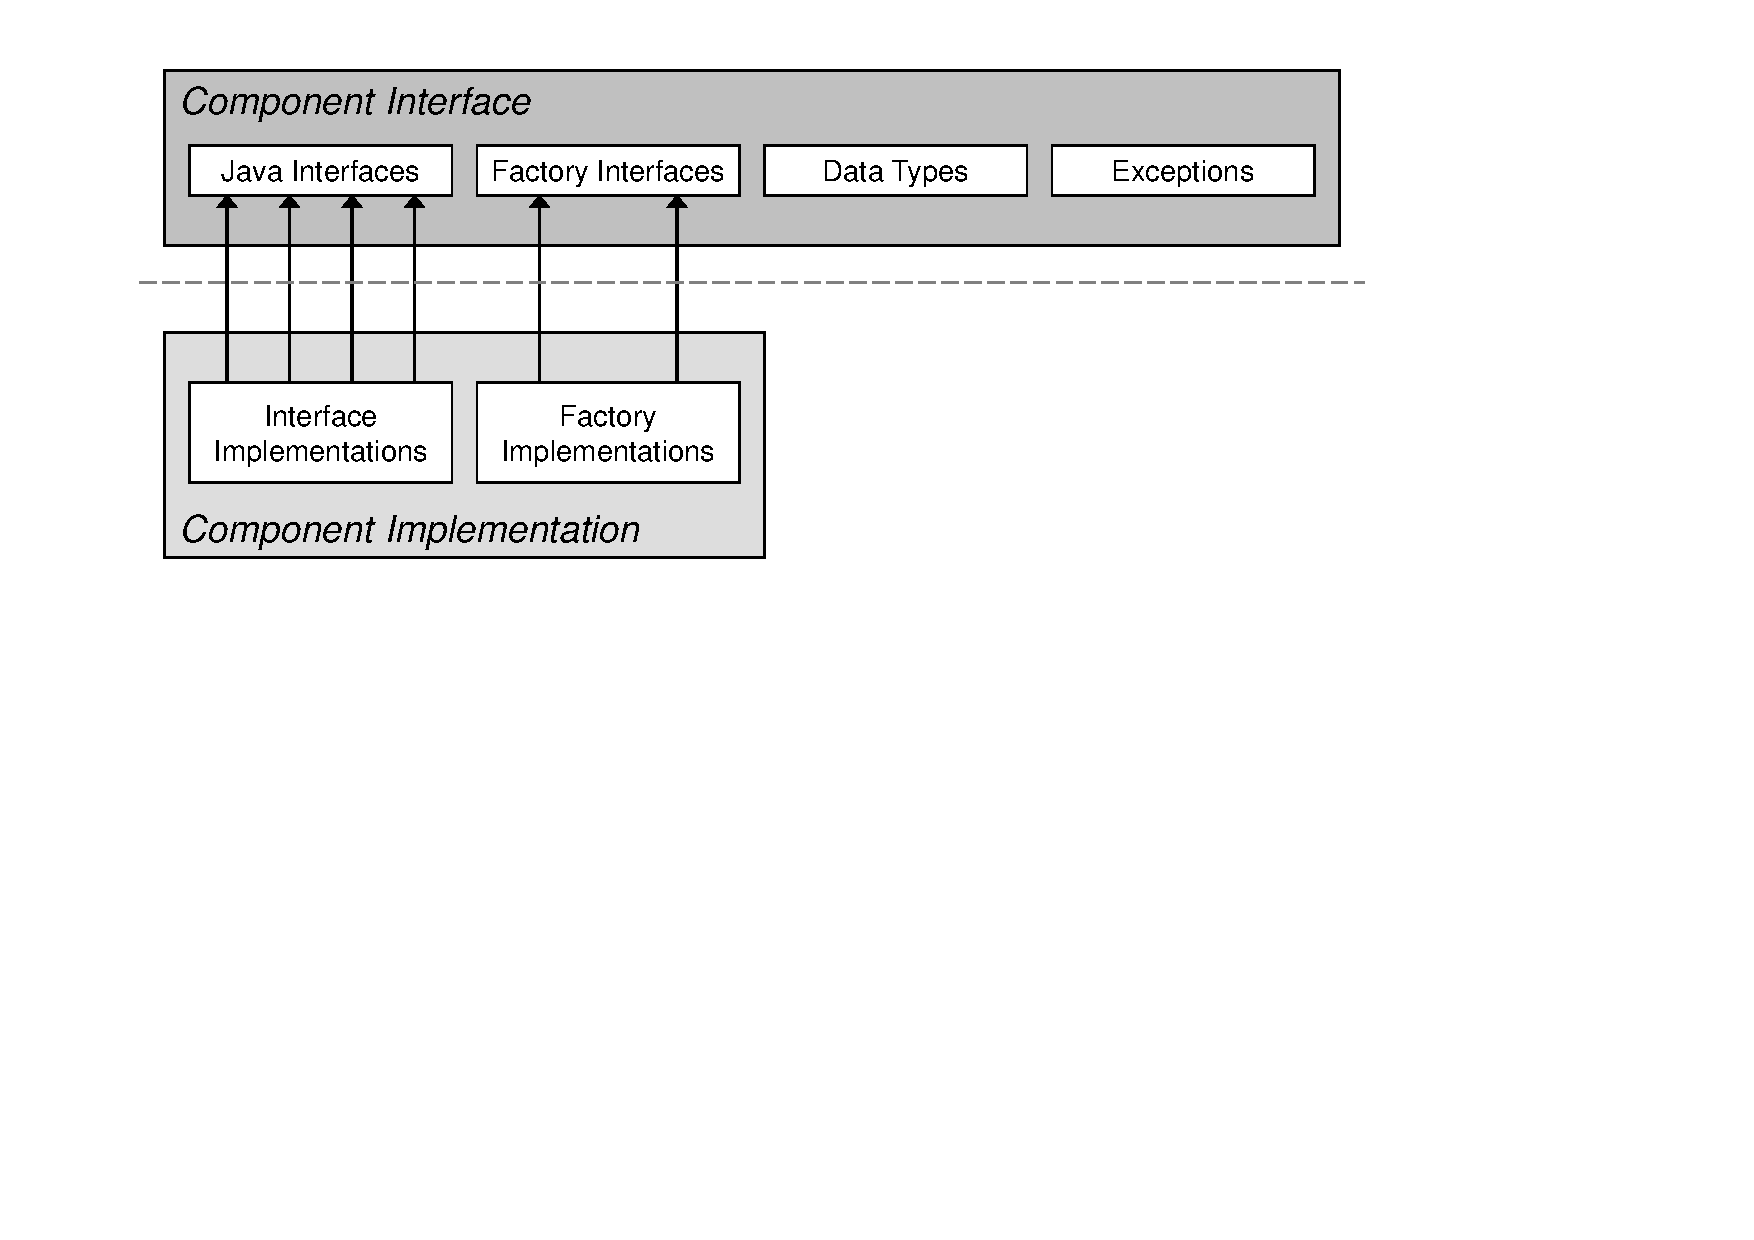
\includegraphics[width=1.00\textwidth]{Figures/Part_II/II_2_ComponentStructure.pdf}
	\caption{Struktur einer Komponente}
	\label{fig:5_3_SCH_Komponente}
\end{figure}

Die Komponentenschnittstelle besteht aus einem oder mehreren Java interfaces, exceptions und Datentypen.
\begin{itemize}
	\item \emph{Java interfaces} stellen die funktionalen API der Komponente dar, jede Methode entspricht einem Service der Komponente. Ein Java interface wird f�r eine klar definierte Unteraufgabe der Komponente genutzt. Manche Interfaces haben Erzeugungscharakter, geben also Zugriff auf andere Interfaces der Komponente.
	\item \emph{Datentypen} sind konstante Java-Klassen, die direkt in implementierungsform zur Verf�gung gestellt werden. Meist dienen sie dazu, Daten zu halten, die als Eingabe oder R�ckgabe verwendet werden.
	\item \emph{Exceptions} sind Fehler die auf funktionelle Fehler hindeuten. Es handelt sich um gepr�fte Exceptions, die an der Service-Schnittstelle definiert werden und vom Anwender behandelt werden m�ssen.
\end{itemize}

%-----------------------------------------------------------------------------------------------
%		Design Decision: Keine Schichtenarchitektur in Komponenten
%-----------------------------------------------------------------------------------------------

\subsection{Designentscheidungen zur Verwendung von Komponenten}
\label{sec:DesVerwKomp}

%-----------------------------------------------------------------------------------------------
%		Design Decision: Entkoppeln von Komponenten �ber ein leichtgewichtiges Service-Locator-Pattern
%-----------------------------------------------------------------------------------------------
\DD{dd:004}
{% Titel
	Entkoppeln von Komponenten �ber ein leichtgewichtiges Service-Locator-Pattern
}
{% Kurzbeschreibung
	Um geringe Kopplung zwischen den Komponenten zu erreichen, d�rfen sich diese nur �ber ihre Komponentenschnittstellen kennen. Dies trifft auch f�r das Erzeugen anderer Komponenten bzw. das Erlangen einer Referenz auf ein anderes Komponenteninterface zu. Um dies zu erreichen, wird ein leichtgewichtiges Service-Locator-Pattern in Form einer eigenen Utility verwendet.
}
{% Begr�ndung
Wir wollen vern�nftige Entkopplung zwischen Komponenten, und daher brauchen wir eine entsprechende Utility. Diese soll leichtgewichtig sein, damit scheiden Java EE und Spring aus, Drittlibraries wie Google Guice ebenso wegen \DesLink{dd:002}.
}
{% Nachteile
 Keine erkennbar
}

%-----------------------------------------------------------------------------------------------
%		Singleton Components
%-----------------------------------------------------------------------------------------------

\DD{dd:005}
{% Titel
	Singleton-Komponenten
}
{% Kurzbeschreibung
	Jede Komponente hat eine einzelnes \emph{Zugriffs-Java-interface}, das wiederum Zugriff auf all Services der Komponente gew�hrt. Dazu kann das Zugriffsinterface Instanzen vefschiedener anderer Klassen oder Interfaces zur�ckliefern, mit denen der Aufrufer dann arbeiten kann.

Aus einer Laufzeit- und Implementierungsperspetive hat jedes der Zugriffs-Java-Interfaces eine Art ``singleton''-Implementierung. Es darf also nur eine Instanz der Zugriffs-Java-Interfaces einer Komponente geben. Nat�rlich darf es im Kontrast dazu mehrere Instanzen jedes anderen Interfaces geben, dass die Komponente definiert.
}
{% Begr�ndung
Die Zugriffs-Java-Interfaces sind nur funktional, und da es nur genau eine Komponentenimplementierung in \LibName{} je Komponente gibt, hat man immer nur eine implementierende Klasse. F�r diese ist zur Laufzeit nur eine Instanz erforderlich, da sie keine Zust�nde h�lt. Dies spart Speicherplatz und Initialisierungsaufwand.
}
{% Nachteile
 Keine erkennbar
}

%-----------------------------------------------------------------------------------------------
%		Design Decision: Entkoppeln von Komponenten �ber ein leichtgewichtiges Service-Locator-Pattern
%-----------------------------------------------------------------------------------------------

\DD{dd:006}
{% Titel
	Unterteilung in Subsysteme
}
{% Kurzbeschreibung
	Eine Ebene �ber den Komponenten untergliedern wir \LibName{} noch in sogenannten \emph{Subsysteme}. Ein Subsystem zerf�llt in Komponenten, und hat sonst keine anderen Inhalte. Es ist also nur eine weitere Gliederungsebene. Generell ist es Komponenten innerhalb desselben Subsystems erlaubt, st�rker an andere Komponenten gekoppelt zu sein, w�hrend Subsysteme untereinander eher �ber eine geringere Kopplung verf�gen sollten. Um dies zu gew�hrleisten, k�nnen Subsysteme sogenannte Fassadenkomponenten anbieten.
}
{% Begr�ndung
Anhand dieser Untergliederung k�nnen wir bereits eine grobe Architektursicht mit den wichtigsten Elementen und Abh�ngigkeiten definieren und auf dieser Basis die Library schrittweise weiter verfeinern.
}
{% Nachteile
 Keine erkennbar
}


%-----------------------------------------------------------------------------------------------
%		Design Decision: API and Implementation Layers
%-----------------------------------------------------------------------------------------------

\DD{dd:007}
{% Titel
	API- und Implementierungs-Layer
}
{% Kurzbeschreibung
	Jede Komponente bietet ihre Dienste, Exceptions und Datentypen �ber einen API-Layer an. Dieser stellt die �ffentliche Schnittstelle der Komponente dar. Andere Komponenten ebenso wie der \LibName{}-Anwender d�rfen die Komponente nur �ber diese API-Klassen verwenden. Der Implementierungs-Layer der Komponente implementiert den API-Layer und ist privat. Insbesondere sind compile-Zeit-Abh�ngigkeiten zu dessen Klassen von anderen Komponenten oder Anwender-Klassen aus verboten.
}
{% Begr�ndung
  Es gibt eine Klare Trennung zwischen privaten und �ffentlichen Anteilen, was die Kopplung und das Risiko von Fehlerpropagation sowie Inkompatibilit�ten verringert, weil sich interne �nderungen an der Komponente idealerweise gar nicht auf nutzende Komponenten auswirken.
}
{% Nachteile
 Keine erkennbar
}

%-----------------------------------------------------------------------------------------------
%		Keine Schichtenarchitektur in der Komponenten-Implementierung
%-----------------------------------------------------------------------------------------------

\DD{dd:008}
{% Titel
	Keine Schichtenarchitektur in der Komponenten-Implementierung
}
{% Kurzbeschreibung
	Die Implementierungs-Schicht einer Komponente in \LibName{} wird nicht weiter in Unter-Schichten gegliedert (wie dies in EE-Anwendungen h�ufig der Fall ist). Die innere Struktur einer Komponente wird durch keine Architekturvorgaben standardisiert, sondern zweckdienlich implementiert. Eine Schichtenarchitektur w�re beispielsweise: Eine Schicht k�mmert sich um das Pr�fen von Vorbedingungen, eine zweite implemeniert die Funktionalit�t, eine dritte k�mmert sich um den Zugriff auf externe Daten.
}
{% Begr�ndung
Eine Schichtenarchitektur in der Komponentenimplementierung ist f�r \LibName{} nicht notwendig und verkompliziert dessen Architektur. Es handelt sich um keine klassische ``3-tier''-Anwendung, sondern eine Hilfslibrary, in welcher nur wenige Komponenten Datenzugriffe durchf�hren. Eine Schichtenarchitektur w�rde zu einer Verringerung der �bersichtlichkeit und mehr Redundanz f�hren, ohne nennenswerte Vorteile bei ``separation of concerns'' oder Entkopplung zu bringen.
}
{% Nachteile
 Keine erkennbar
}

%-----------------------------------------------------------------------------------------------
%		Design Decision: Entwicklungsumgebung
%-----------------------------------------------------------------------------------------------

\section{Entwicklungsumgebung}
\label{sec:entw}

\DD{dd:009}
{% Titel
	Entwicklungsumgebung
}
{% Kurzbeschreibung
	Als Entwicklungsumgebung wird eine Kombination aus Eclipse, Maven und Subversion genutzt.
}
{% Begr�ndung
Bekannte und kostenloste Toolsuite.
}
{% Nachteile
 Keine erkennbar
}

%-----------------------------------------------------------------------------------------------
%		Design Decision: Multithreading
%-----------------------------------------------------------------------------------------------

\section{Multithreading}
\label{sec:mult}

\DD{dd:010}
{% Titel
	\LibName{} ist nicht thread-safe
}
{% Kurzbeschreibung
	\LibName{} ist keine thread-safe Library und verwendet keine Java-APIs, die thread-safe sind.
}
{% Begr�ndung
Thread-Sicherheit bedeutet ggf. Performance-Verringerung durch Erzeugung von Synchronisationspunkten und Erh�hung der Gesamtkomplexit�t. Single-thread-Anwendungen werden benachteiligt. Es ist schwierig, thread-safety \emph{korrekt} umzusetzen. Anwender k�nnen selbst daf�r Sorge tragen, dass ihre multi-threaded-Anwendung thread-safe ist.
}
{% Nachteile
Keine erkennbar
}

%-----------------------------------------------------------------------------------------------
%		Design Decision: Architektur
%-----------------------------------------------------------------------------------------------

\section{Architektur}
\label{sec:arch}

\DD{dd:011}
{% Titel
	Architektur von \LibName{}
}
{% Kurzbeschreibung
	\LibName{} basiert auf der technischen und fachlichen Architektur, wie sie in den Kapiteln \SectionLink{sec:TechnicalArchitectureChap} und \SectionLink{sec:FunctionalArchitectureChap} definiert wird.
}
{% Begr�ndung
Siehe Diskussion der Architektur im Detail in den n�chsten Abschnitten.
}
{% Nachteile
Siehe Diskussion der Architektur im Detail in den n�chsten Abschnitten.
}

%###############################################################################################
%###############################################################################################
%
%		File end
%
%###############################################################################################
%###############################################################################################
%===============================================================================================
%		Technische Archiktur
%===============================================================================================

\chapter{Technische Architektur}
\label{sec:TechnicalArchitectureChap}

%-----------------------------------------------------------------------------------------------
%		Technische Infrastruktur
%-----------------------------------------------------------------------------------------------

\section{Technische Infrastruktur}
\label{sec:TechnicalInfrastructure}

Die technische Infrastruktur beschreibt die Umgebung, die f�r das Arbeiten mit \LibName{} ben�tigt wird, wie in der folgenden Abbildung gezeigt:

\begin{figure}[H]
	\centering
		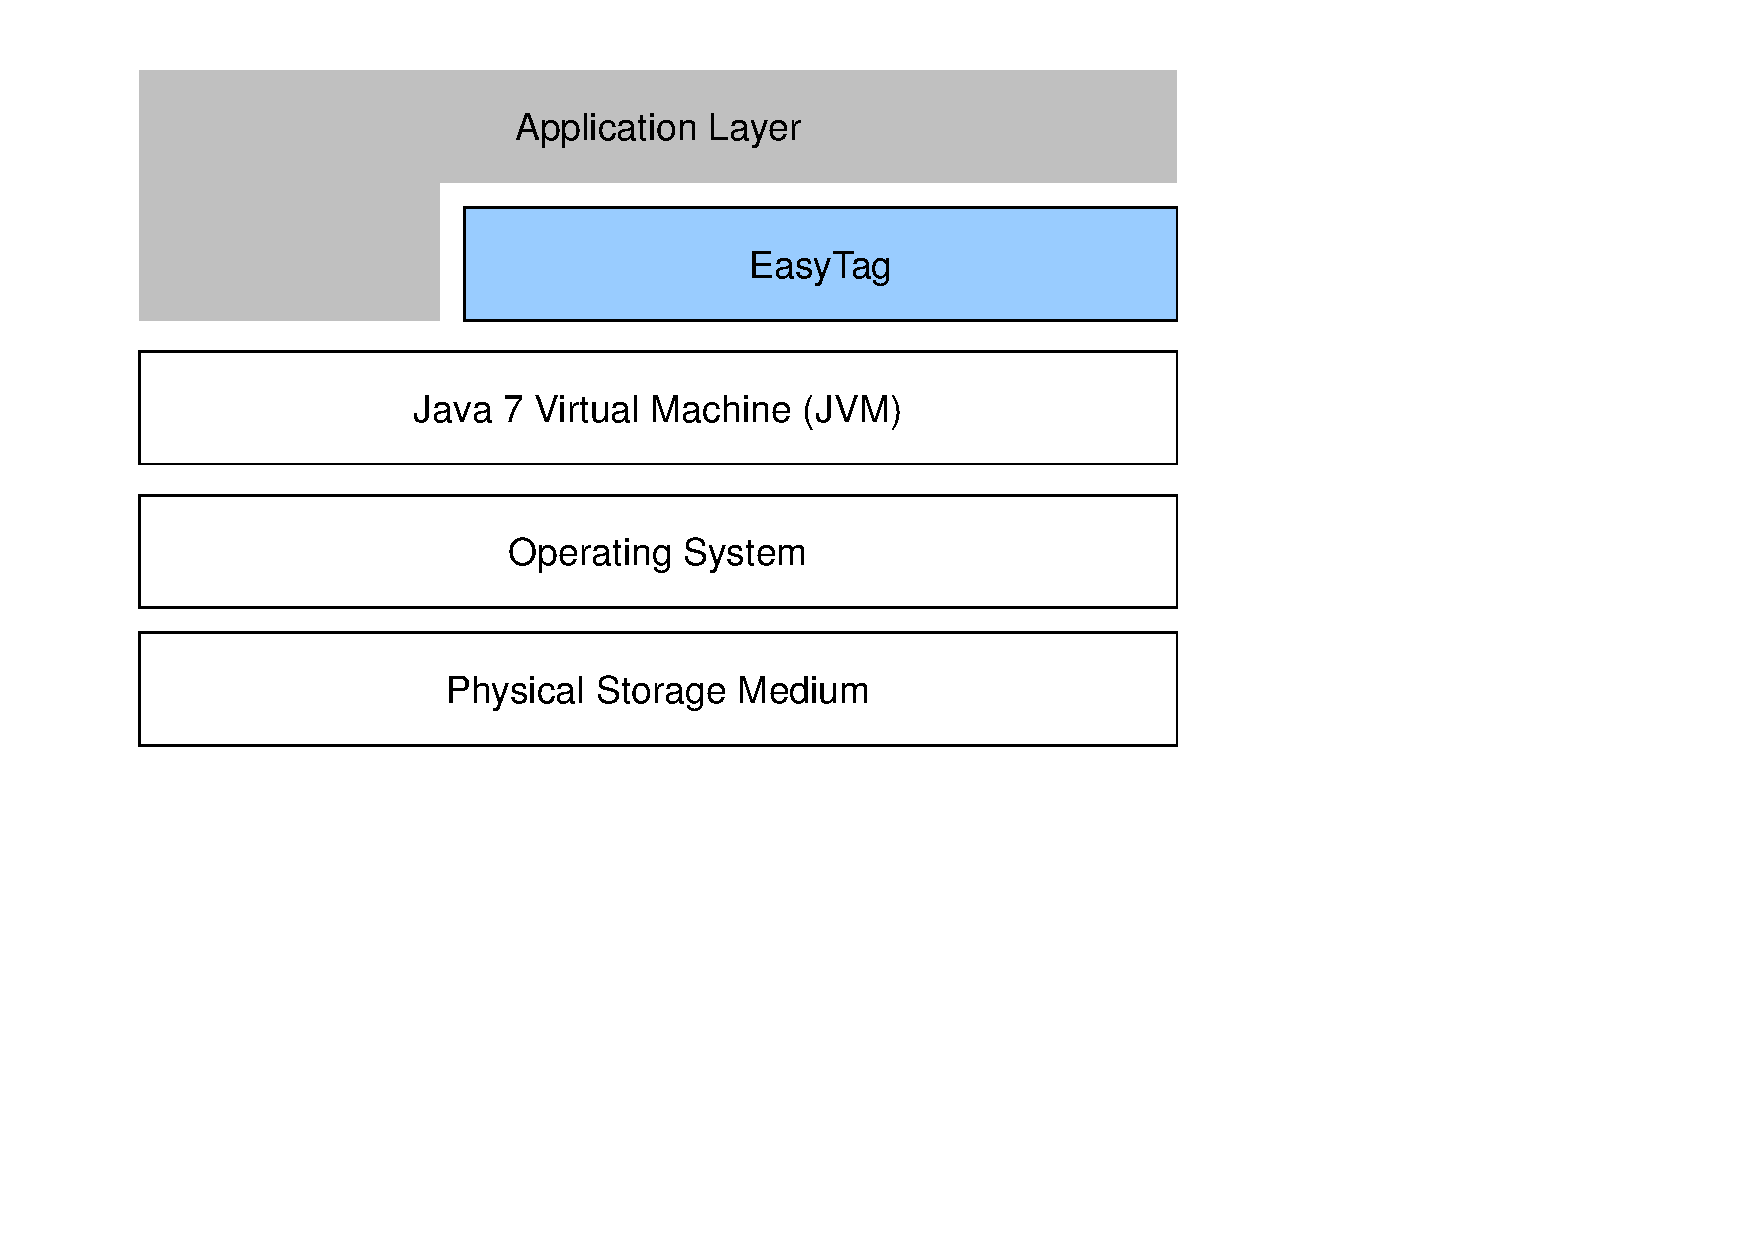
\includegraphics[width=1.00\textwidth]{Figures/Part_II/II_1_TechnicalInfrastructure.pdf}
		\caption{Technische Infrastruktur von \LibName{}}
	\label{fig:5_3_SCH_TechnicalInfrastructure}
\end{figure}

Die technische Schichtenstruktur kann als Abh�ngigkeits- und Kommunikationsstruktur interpretiert werden. Der Applikations-Layer basiert auf \LibName{} w�hrend sowohl \LibName{} als auch der Applikations-Layer die \JavaVersion{} benutzen. \JavaVersion{} greift auf das Betriebssystem zu, welches Dienste zum Zugriff auf das physische Medium bietet.

Die Schichten sollten dabei nur auf benachbarte Schichten zugreifen.

%-----------------------------------------------------------------------------------------------

\subsection{Application Layer}
\label{sec:ApplicationLayer}

Der Application Layer ist die Software, die \LibName{} zum Extrahieren und Schreiben von Metadaten nutzt. Es handelt sich um eine Java-Anwendung, mindestens f�r \JavaVersion{} entwickelt worden ist. Sie nutzt nat�rlich dar�ber hinaus andere Java-Funktionalit�t und Libraries. Es kann sich um eine Java-SE-Desktop-Applikation oder auch eine Java-EE-Server-Applikation handeln.

%-----------------------------------------------------------------------------------------------

\subsection{\LibName{}}
\label{sec:LibName}

In der Abbildung bezeichnet \LibName{} alle Laufzeitkomponenten der Library \LibName{}. Diese Komponenten werden vom Application Layer aufgerufen und genutzt. \LibName{} selbst ist eine reine Java Library, die auf der \JavaVersion{} Java Virtual Machine (JVM) l�uft. Sie kann somit nicht mit �lteren Java-Versionen eingesetzt werden.

%-----------------------------------------------------------------------------------------------

\subsection{Java Virtual Machine (JVM)}
\label{sec:JavaVirtualMachineJVM}

\LibName{} ben�tigt eine Java Virtual Machine (JVM). \LibName{} wird in \JavaVersion{} entwickelt und ist daher nicht auf fr�heren Versionen nutzbar.

%-----------------------------------------------------------------------------------------------

\subsection{Betriebssystem}
\label{sec:OperatingSystem}

Die JVM l�uft auf jedem Betriebssystem, das \JavaVersion{} unterst�tzt. Daher entkoppelt die JVM \LibName{} vom Betriebssystem. Es gibt jedoch einige Systemfunktionalit�ten wie Prozess- und Threadmanagement ebenso wie Dateisystemzugriff, die teilweise vom Betriebssystem abh�ngen.

%-----------------------------------------------------------------------------------------------

\subsection{Physisches Speichermedium}
\label{sec:PhysicalStorageMedium}

\LibName{} greift auf Daten zu, die auf einem physischen Speichermedium gespeichert sind. Seine Lage oder Art ist unterschiedlich. In vielen F�llen handelt es sich um eine Datei auf einer Festplatte, es k�nnte sich aber auch um eine entfernt gespeicherte Ressource, Hauptspeicher oder eine Datenbanktabelle in einer entfernten Datenbank handeln.

Der Application Layer muss bei Verwendung von \LibName{} niemals selbst auf das physische Medium zugreifen. \LibName seinerseits nutzt die \JavaVersion{}, diese das Betriebssystem, um auf die Daten des Mediums zuzugreifen.

%-----------------------------------------------------------------------------------------------
%		Technische Basiskomponenten
%-----------------------------------------------------------------------------------------------

\section{Technische Basiskomponenten}
\label{sec:TechnicalBasis}

Technische Basiskomponenten dienen nur als Hilfsmittel oder Rahmen der Umsetzung der fachlichen Inhalte von \LibName{}. Unter ``fachliche'' Inhalte wird das Lesen und Schreiben von Metadaten und das Lesen von Container-Daten verstanden. Die daf�r notwendigen technischen Basiskomponenten werden hier kurz aufgef�hrt:
\begin{itemize}
	\item Logging
	\item Service-Locator
	\item Utility
	\item Verwaltung von Erweiterungen
\end{itemize}

Details zu diesen Komponenten findet sich in \SectionLink{sec:Design}.

%###############################################################################################
%###############################################################################################
%
%		File end
%
%###############################################################################################
%###############################################################################################
%===============================================================================================
%		Fachliche Architektur
%===============================================================================================

\chapter{Fachliche Architektur}
\label{sec:FunctionalArchitectureChap}

Die fachliche Architektur umfasst die Gliederung der Library-Funktionalit�t in fachliche Einheiten. Auf detaillierter Ebene sind dies die bereits definierten Komponenten. Auch wenn diese rein technische Funktionen umsetzen, beispielsweise Logging, werden sie in der fachlichen Architektur aufgef�hrt.

Hier noch einige detaillierte Designentscheidungen, die sich auf die fachliche Architektur beziehen.

%-----------------------------------------------------------------------------------------------
%		Grundlegende Designentscheidungen zur fachlichen Architektur
%-----------------------------------------------------------------------------------------------

\section{Grundlegende Designentscheidungen zur fachlichen Architektur}
\label{sec:Grld}

Die folgenden grundlegenden Designentscheidungen haben einen ma�geblichen Einfluss auf die fachliche Architektur der Library, und sie haben einen �bergreifenden Effekt, sind also nicht auf einzelne Subsysteme oder Komponenten beschr�nkt. Daher werden sie hier definiert. Sie liefern eine generelle Begr�ndung des sp�ter entwickelten fachlichen Designs.

%-----------------------------------------------------------------------------------------------

\DD{dd:100}
{% Titel
	High-Level- und Low-Level-API
}
{% Kurzbeschreibung
	Wir untergliedern \LibName{} in einen High-Level-Anteil, der bequeme User-Funktionalit�t zum Zugriff auf Metadaten bietet, und einen Low-Level-Anteil, der generische Expertenfunktionalit�t auf Bit- und Byte-Ebene bietet.
}
{% Begr�ndung
Zun�chst muss eine Low-Level-Zugriffsm�glichkeit gem��t \SectionLink{sec:ANF004ZugriffAufAlleRohdatenUeberDieLibrary} zur Vergf�gung gestellt werden. Statt Low-Level- und High-Level-Zugriff in einer un�bersichtlichen API gemeinsam bereitzustellen, separieren wir sowohl API als auch die Implementierung dieser Belange. Aus Anwendersicht ist dann klar, welche API f�r ihn als ``bequem'' gedacht ist, und welche nur f�r detaillierten feingranularen Zugriff verwendet werden soll. Die low-level-API kann von der High-level-API aufgerufen werden, um diese zu implementieren. Dies schafft auch eine saubere Trennung in der Implementierung.
}
{% Nachteile
Ggf. h�here Komplexit�t der Gesamtl�sung
}

%-----------------------------------------------------------------------------------------------

\DD{dd:101}
{% Titel
	Generisches Parsen und Schreiben anhand einer Format-Spezifikation
}
{% Kurzbeschreibung
	Das Parsen und Schreiben s�mtlicher Metadaten- und Container-Formate wird anhand einer generellen Format-Spezifikation durch eine zentrale Komponente durchgef�hrt. Die Format-Spezifikation beschreibt, welche Features und Teile ein bin�res Datenformat enth�lt, insbesondere, wie ein Datenblock dieses Formates aufgebaut ist und interpretiert werden muss. Es handelt sich also um eine Art generische Anleitung f�r das Parsen (und auch das Schreiben und Validieren) dieses Datenformates.

Weitere Designentscheidungen in sp�teren Abschnitten werden diese Designentscheidung vertiefen.
}
{% Begr�ndung
Gem�� dem Dokument \cite{MetaComp} haben zumindest bin�re Container- und Metadatenformate viele Gemeinsamkeiten, die unter anderem die Definition eines generellen Dom�nenmodells erm�glichen. Diese Gemeinsamkeiten lassen sich auch durch generelle Formatspezifikationen beschreiben. Statt f�r jedes neu zu unterst�tzende Datenformat komplett neuen Parse-Code schreiben zu m�ssen, k�nnen viele Formate durch einheitlichen (nur einmal zu testenden) generischen Parse-Code unterst�tzt werden. Es ist eine Entkopplung von Format-Beschreibung und Lesen/Schreiben m�glich. Die Formatbeschreibung kann als Textdokument abgelegt werden. Eine Erweiterung um ein neues Format ist daher im Idealfall einzig und allein durch Erzeugen einer solchen konformen Textdatei umsetzbar. Somit erm�glicht diese Designentscheidung die Umsetzung der Anforderung \SectionLink{sec:ANF007ErweiterbarkeitUmNeueMetadatenUndContainerformate}.
}
{% Nachteile
Es kann nicht f�r jedes denkbare zuk�nftige Format sichergestellt werden, dass die M�glichkeiten der Format-Spezifikation ausreichen, um alle Features des jeweiligen Formates wirklich abzudecken. Dies kann zur Notwendigkeit f�hren, die Format-Spezifikation zu erweitern und damit auch das generische Parsen. Alternativ kann dies durch M�glichkeiten ausgeglichen werden, das Parsen doch selbst umzusetzen (und eine entsprechende Implementierung statt der generischen zu verwenden). Weiterer Nachteil: Evtl. leichter Performance-Verlust, da das generische Parsen nat�rlich viele verschiedene F�lle unterst�tzen muss.
}

%-----------------------------------------------------------------------------------------------

\DD{dd:102}
{% Titel
	�berschreiben des generischen Parsens und und Schreibens
}
{% Kurzbeschreibung
	Erweiterungen k�nnen f�r ihre Datenformate den generischen Lese- und Schreibvorgang (siehe \DesLink{dd:101}) �berschreiben und erweitern, um sie an spezielle Gegebenheiten ihres Datenformates besser anzupassen.
}
{% Begr�ndung
Dies minimiert die Nachteile von \DesLink{dd:101} und erm�glicht in Einzelf�llen einfacherer oder performantere Implementierungen.
}
{% Nachteile
Keine erkennbar
}

%-----------------------------------------------------------------------------------------------

\DD{dd:103}
{% Titel
	Format-Spezifika werden nur in Erweiterungen definiert
}
{% Kurzbeschreibung
	Jegliche Spezifika eines Metadaten- oder Containerformates werden ausschlie�lich �ber Erweiterungen implementiert, das gilt selbst f�r Datenformate, die direkt mit der Kernversion von \LibName{} unterst�tzt werden.
}
{% Begr�ndung
So wird bereits mit der Kernlibrary selbst das Erweiterungskonzept genutzt und erprobt. Es findet eine strikte Trennung zwischen Kernimplementierung und Format-Spezifika statt, was eine bessere Beherrschung der Gesamt-Komplexit�t erm�glicht.
}
{% Nachteile
Keine erkennbar
}

%-----------------------------------------------------------------------------------------------

\DD{dd:104}
{% Titel
	Fassadenkomponenten f�r High-Level- und Low-Level-Anteile
}
{% Kurzbeschreibung
	Die Subsysteme \SUBSHighLevel{} und \SUBSLowLevel{} verf�gen �ber je eine Fassadenkomponente, die Zugriff auf die anderen \emph{�ffentlichen} Komponenten des jeweiligen Subsystems gew�hren. ``�ffentlich'' sind diejenigen Komponenten, die vom Anwender oder von \SUBSBootstrap{} direkt zugegriffen werden m�ssen.
}
{% Begr�ndung
Das Subsystem \SUBSBootstrap{} muss keine direkte Abh�ngkeit zu den Komponenten der Subsysteme der High-Level- und Low-Level-Anteile eingehen, sondern gibt nur eine Instanz der Fassadenkomponenten zur�ck, dies verringert die Kopplung. Spezielle Methoden zum Zugriff auf die anderen Komponenten des Subsystems k�nnen in den Fassadenkomponenten bereitgestellt werden und m�ssen nicht im Subsystem \SUBSBootstrap{} bereitgestellt werden (was auch nicht der Aufgabe von \SUBSBootstrap{} entsprechen w�rde).
}
{% Nachteile
Keine erkennbar
}

%-----------------------------------------------------------------------------------------------

\DD{dd:105}
{% Titel
	Technische Basiskomponenten bilden ein eigenes Subsystem ohne Fassade
}
{% Kurzbeschreibung
	Alle technischen Basiskomponenten bilden ein eigenes Subsystem und werden nicht zusammen mit fachlichen Komponenten in ein Subsystem aufgenommen. Es wird keine Fassadenkomponente zum Zugriff auf die Basiskomponenten bereitgestellt.
}
{% Begr�ndung
Um die Koh�renz der Subsysteme zu erhalten, werden die technischen Komponenten in ein eigenes Subsystem ausgelagert. Die technischen Basiskomponenten k�nnen als sogenannte ``0-Software'', d.h. perfekt wiederverwendbare Software betrachtet werden. Sie haben keine inhaltlich-fachliche Funktionen und sollten (in den meisten F�llen) keine weiteren Abh�ngigkeiten zu anderen Komponenten haben. Da sie alle recht spezifische und umfangreiche Funktionalit�t anbieten, macht ein Verwenden einer Fassadenkomponenten keinerlei Sinn. Diese w�rde einerseits viele unterschiedliche Belange, die nicht verwandt sind, in ein Interface zw�ngen, und andererseits  keineswegs zu geringerer Kopplung f�hren.
}
{% Nachteile
Keine erkennbar
}

%-----------------------------------------------------------------------------------------------
%		Subsysteme
%-----------------------------------------------------------------------------------------------

\section{Subsysteme}
\label{sec:Subsystems}

Die Unterteilung in Subsysteme zeigt bereits grob die wichtigsten Teile der Library und erste Abh�ngigkeiten zwischen ihnen. �ber Subsysteme verorten wir auch den Begriff der \emph{Erweiterung}. Zudem bildet sich hier direkt die Designentscheidung \DesLink{dd:100} ab.

Das folgende Architekturbild zeigt die Subsysteme von \LibName{} und ihre Beziehungen zueinander. Ein Pfeil bedeutet dabei eine hier noch nicht n�her konkretisierte Abh�ngigkeit, die sich entweder als Compile-Zeit- oder als Laufzeit-Abh�ngigkeit oder beides manifestieren kann.

\begin{figure}[H]
	\centering
		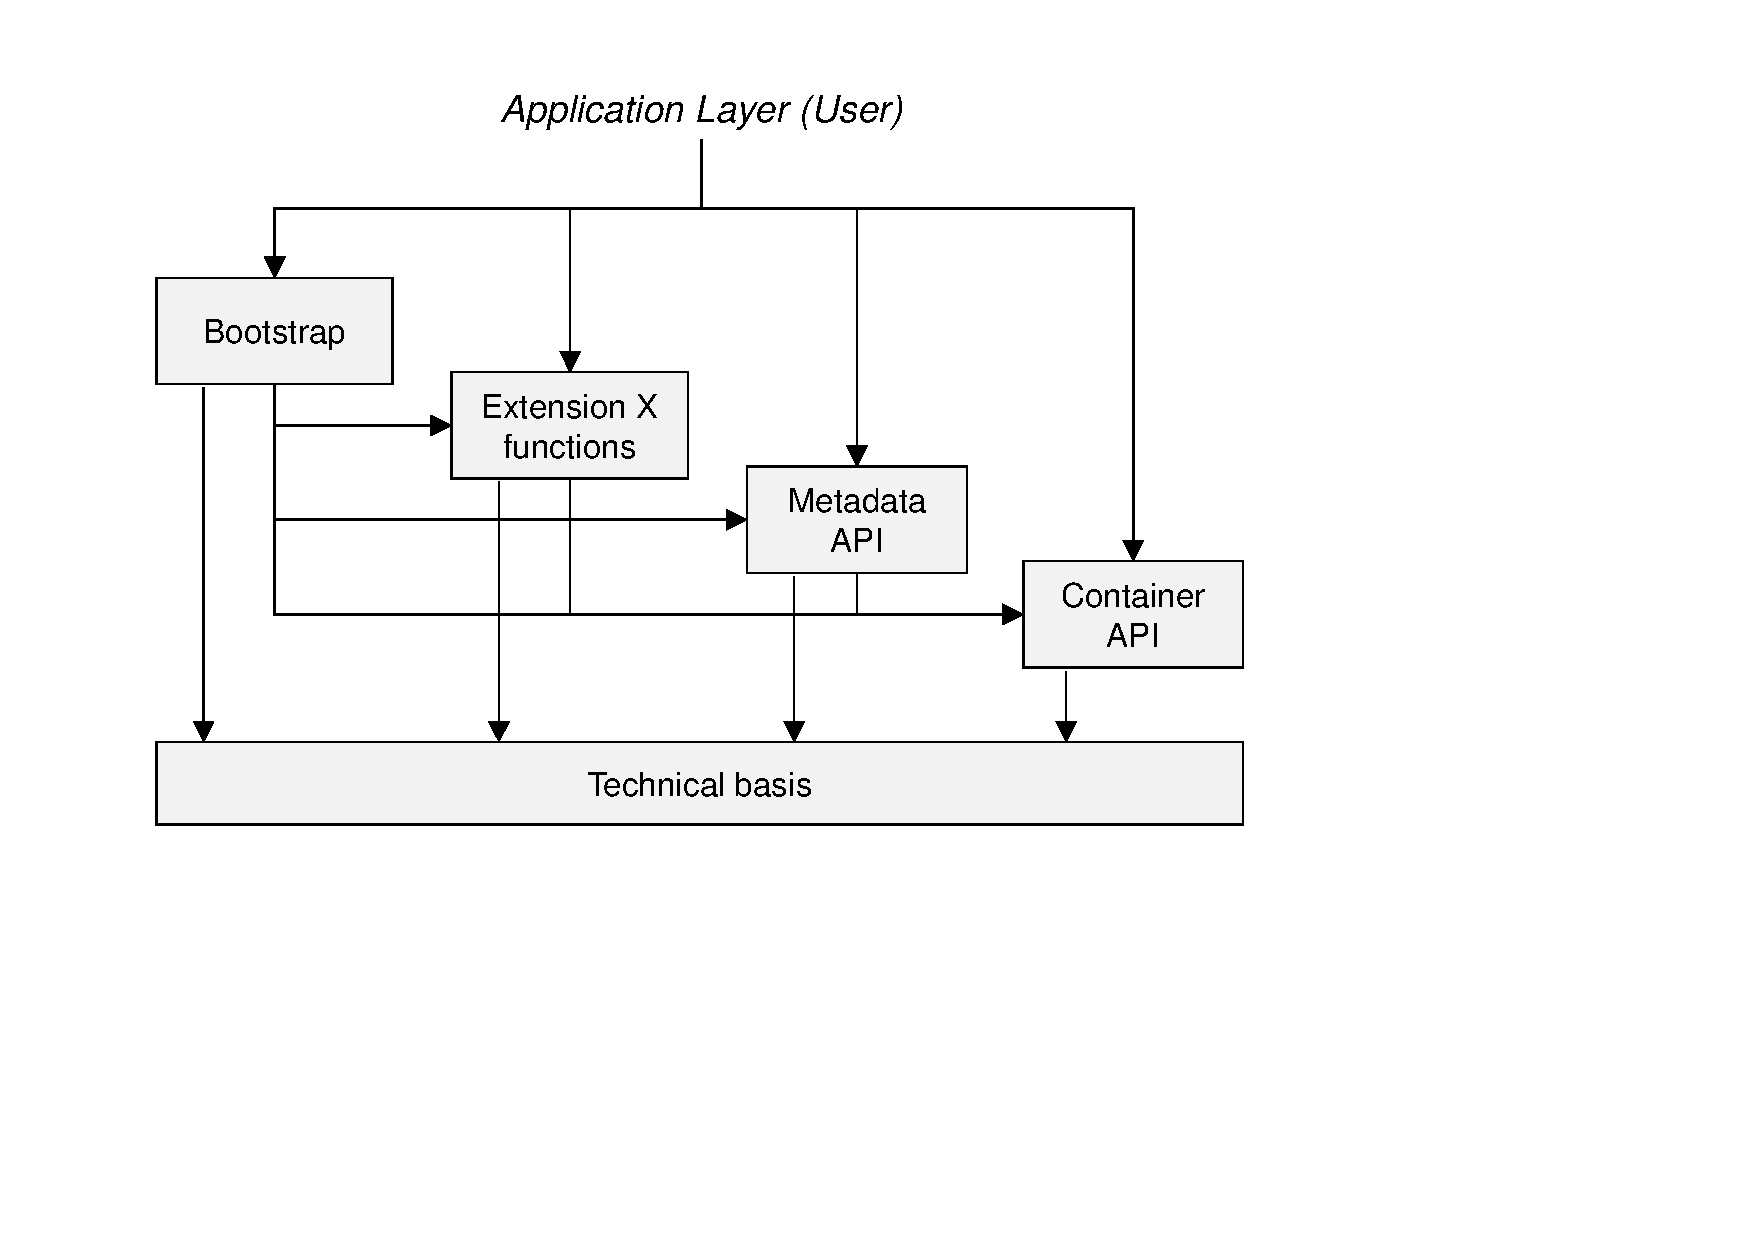
\includegraphics[width=1.00\textwidth]{Figures/Part_II/II_1_FunctionalArchitecture.pdf}
		\caption{Subsysteme von \LibName{}}
	\label{fig:5_3_SCH_TechnicalArchitecture}
\end{figure}

Der Anwender der Library kann direkt auf die Subsysteme \SUBSBootstrap{}, \SUBSExtension{}, \SUBSHighLevel{} und \SUBSLowLevel{} zugreifen, w�hrend die \SUBSTechBase{} nicht zugreifbar ist.

Die Subsysteme werden im Folgenden weiter konkretisiert.

%-----------------------------------------------------------------------------------------------

\subsection{\SUBSBootstrap{}}
\label{sec:Bootstrap}

Dieses Subsystem kapselt alle Initialisierungen von \LibName{}. Das Subsystem ist der Eintrittspunkt der Benutzung von \LibName{} f�r den Anwender. Es nutzt daher alle anderen Subsysteme, um diese zu initialisieren.

Die Komponenten des Subsystems sind im Abschnitt \SectionLink{sec:KompBoots} aufgef�hrt.

%-----------------------------------------------------------------------------------------------

\subsection{\SUBSHighLevel{}}
\label{sec:LibName2}

Die High-Level-Anteile der Library gem�� \DesLink{dd:100}. Das Subsystem greift auf \SUBSTechBase{} und \SUBSLowLevel{} zu. Letzteres deshalb, weil gem�� \DesLink{dd:100} die Implementierung der High-Level-Anteile durch Verwendung der low-level-Anteile erfolgt.

Die Komponenten des Subsystems sind im Abschnitt \SectionLink{sec:KompHigh} aufgef�hrt.

%-----------------------------------------------------------------------------------------------

\subsection{\SUBSLowLevel{}}
\label{sec:CoreAndUserInterface}

Die Low-Level-Anteile der Library gem�� \DesLink{dd:100}. Greift nur auf die technische Basis zu.

Die Komponenten des Subsystems sind im Abschnitt \SectionLink{sec:KompLow} aufgef�hrt.

%-----------------------------------------------------------------------------------------------

\subsection{\SUBSTechBase{}}
\label{sec:Techbase}

Eine Sammlung von Komponenten, die als technische Rahmenkomponenten betrachtet werden k�nnen und keine fachlich-inhaltlichen Beitr�ge zum Thema ``Metadaten/Container'' liefern. Sie werden von so gut wie allen anderen Subsystemen ben�tigt.

Die Komponenten des Subsystems sind im Abschnitt \SectionLink{sec:KompTB} aufgef�hrt.

%-----------------------------------------------------------------------------------------------

\subsection{\SUBSExtension{}}
\label{sec:Extensions}

\LibName{} erlaubt eine beliebige Anzahl an Erweiterungen, jede davon entspricht in der fachlichen Architektur einem Subsystem.

Details finden sich im Abschnitt \SectionLink{sec:KompExt}.

%-----------------------------------------------------------------------------------------------
%		Komponenten-Steckbrief
%-----------------------------------------------------------------------------------------------

\section{Komponenten-Steckbrief}
\label{sec:StructureofaComponentDescription}

Da in den folgenden Abschnitten Komponenten einf�hrend beschrieben werden, wird hier ein Steckbrief, d.h. eine grundlegende Beschreibungsstruktur f�r eine Komponentengrobbeschreibung definiert. Dieser Steckbrief wird dann in den folgenden Abschnitten f�r jede Komponente ausgef�llt.

\textbf{Komponenten-Name:} Der Name der Komponente.

\textbf{Aufgabe:} Die Aufgabe der Komponente.

\textbf{Kontrollierte Daten:} Die Daten, die durch die Komponente kontrolliert werden, d.h. gelesen und geschrieben werden. Nutzt die Komponente Daten anderer Komponenten, wird dies hier nicht erw�hnt.

\textbf{Abh�ngig von $<$Komponenten-Name$>$:} Dieses Element kommt mehrfach je Komponente vor, von der diese Komponente abh�ngt. Der Grund f�r die Abh�ngigkeit wird kurz erl�utert.

%-----------------------------------------------------------------------------------------------
%		Komponenten des Subsystems \SUBSBootstrap{}
%-----------------------------------------------------------------------------------------------

\section{Komponenten des Subsystems \SUBSBootstrap{}}
\label{sec:KompBoots}

Die folgende Abbildung zeigt die Komponenten des Subsystems \SUBSBootstrap{}.

\OpenIssue{Bootstrap subsystem Componenten Abbildung}{}
%\begin{figure}[H]
	%\centering
		%\includegraphics[width=1.00\textwidth]{Figures/Part_III/III_1_SUBSBootstrap.pdf}
	%\caption{Komponenten des Subsystems \SUBSBootstrap{}}
	%\label{fig:CompSB}
%\end{figure}

%-----------------------------------------------------------------------------------------------

\subsection{Komponente \COMPcontext{}}
\label{sec:COMPContext}

\textbf{Komponenten-Name:} \COMPcontext{}.

\textbf{Aufgabe:} Der Einstiegspunkt f�r jeden User von \LibName{}. Es erm�glicht Zugriff auf alle anderen Komponenten der Library.

\textbf{Kontrollierte Daten:} Keine.

\textbf{Abh�ngig von \COMPlowLevel{}:} \COMPcontext{} gibt Zugriff auf die Komponente \COMPlowLevel{}.

\textbf{Abh�ngig von \COMPhighLevel{}:} \COMPcontext{} gibt Zugriff auf die Komponente \COMPhighLevel{}.

\textbf{Abh�ngig von \COMPextensionManagement{}:} \COMPcontext{} l�dt alle Erweiterungen unter Nutzung dieser Komponente.

\textbf{Abh�ngig von \COMPlogging{}:} \COMPcontext{} nutzt diese Komponente zur Protokollierung des Startup-Prozesses.

\textbf{Abh�ngig von \COMPcomponentRegistry{}:} \COMPcontext{} nutzt diese Komponente zum Instantiieren bzw. Abfragen von Implementierungen anderer verwendeter Komponenten-Interfaces.

\textbf{Abh�ngig von \COMPutility{}:} \COMPcontext{} nutzt diverse querschnittliche Funktionen von \COMPutility{}.

%-----------------------------------------------------------------------------------------------
%		Komponenten des Subsystems \SUBSHighLevel{}
%-----------------------------------------------------------------------------------------------

\section{Komponenten des Subsystems \SUBSHighLevel{}}
\label{sec:KompHigh}

Die Komponenten des Subsystems \SUBSHighLevel{} werden in dieser Version der Library noch nicht definiert.

%-----------------------------------------------------------------------------------------------
%		Komponenten des Subsystems \SUBSLowLevel{}
%-----------------------------------------------------------------------------------------------

\section{Komponenten des Subsystems \SUBSLowLevel{}}
\label{sec:KompLow}

Die folgende Abbildung zeigt die Komponenten des Subsystems \SUBSLowLevel{}.
\OpenIssue{Container API subsystem Abbildung}{}

%\begin{figure}[H]
	%\centering
		%\includegraphics[width=1.00\textwidth]{Figures/Part_III/III_1_SUBSLowLevel.pdf}
	%\caption{Komponenten des Subsystems \SUBSLowLevel{}}
	%\label{fig:CompLL}
%\end{figure}

%-----------------------------------------------------------------------------------------------

\subsection{\COMPlowLevel{}}
\label{sec:COMPlowLevel}

\textbf{Komponenten-Name:} \COMPlowLevel{}.

\textbf{Aufgabe:} Fassadenkomponente. Gew�hrt allen Anwendern Zugriff auf die anderen �ffentlichen Komponenten dieses Subsystems.

\textbf{Kontrollierte Daten:} Keine.

\textbf{Abh�ngig von \COMPdataPartManagement{}:} Gew�hrt Zugriff auf diese Komponente.

\textbf{Abh�ngig von \COMPdataFormatManagement{}:} Gew�hrt Zugriff auf diese Komponente.

%-----------------------------------------------------------------------------------------------

\subsection{\COMPdataPartManagement{}}
\label{sec:COMPdataPartManagement}

\textbf{Komponenten-Name:} \COMPdataPartManagement{}.

\textbf{Aufgabe:} Gew�hrt lesenden Zugriff auf Metadaten und Containerdaten und schreibenden Zugriff auf Metadaten auf Bit- und Byte-Ebene, allerdings werden die Daten in handlichen Portionen gem�� Datenformat-Spezifikation geliefert.

\textbf{Kontrollierte Daten:} Ein Zugriff auf \TERMcontainer{}- und \TERMtag{}-Daten ist nur �ber diese Komponente erlaubt. Somit hat sie die Kontrolle �ber diese Daten. Lediglich \COMPmedia{} darf auf noch generischerer Ebene auf Daten externer Medien zugreifen. Tats�chlich nutzt \COMPdataPartManagement{}  \COMPmedia{} f�r das Lesen und Schreiben.

\textbf{Abh�ngig von \COMPmedia{}:} \COMPdataPartManagement{} muss Datenpakete von Medien lesen oder auf diese Schreiben. Dazu nutzt es \COMPmedia{}.

\textbf{Abh�ngig von \COMPdataFormatManagement{}:} Das Lesen und Schreiben der Daten erfolgt anhand von Format-Spezifikationen, die durch \COMPdataFormatManagement{} geliefert werden.

%-----------------------------------------------------------------------------------------------

\subsection{\COMPdataFormatManagement{}}
\label{sec:COMPdataFormatManagement}

\textbf{Komponenten-Name:} \COMPdataFormatManagement{}.

\textbf{Aufgabe:} Verwaltet die konkreten Datenformat-Definitionen aller unterst�tzten Metadaten- und Container-Formate.

\textbf{Kontrollierte Daten:} Hat Kontrolle �ber die Datenformat-Definitions-Daten.

\textbf{Abh�ngig von:} Keinen anderen Komponenten.

%-----------------------------------------------------------------------------------------------

\subsection{\COMPmedia{}}
\label{sec:COMPmediumAccess}

\textbf{Komponenten-Name:} \COMPmedia{}.

\textbf{Aufgabe:} Bietet Primitive f�r den Zugriff auf physische Medien an.

\textbf{Kontrollierte Daten:} Daten von externen Medien d�rfen nur �ber diese Komponente zugegriffen und manipuliert werden.

\textbf{Abh�ngig von:} Keinen anderen Komponenten.

%-----------------------------------------------------------------------------------------------
%		Komponenten des Subsystems \SUBSTechBase{}
%-----------------------------------------------------------------------------------------------

\section{Komponenten des Subsystems \SUBSTechBase{}}
\label{sec:KompTB}

Die folgende Abbildung zeigt die Komponenten des Subsystems \SUBSTechBase{}.
\OpenIssue{Tech Base subsystem Abbildung}{}
%\begin{figure}[H]
	%\centering
		%\includegraphics[width=1.00\textwidth]{Figures/Part_III/III_1_SUBSTechBase.pdf}
	%\caption{Komponenten des Subsystems \SUBSTechBase{}}
	%\label{fig:CompTB}
%\end{figure}

%-----------------------------------------------------------------------------------------------

\subsection{\COMPextensionManagement{}}
\label{sec:COMPextensionManagement}

\textbf{Komponenten-Name:} \COMPextensionManagement{}.

\textbf{Aufgabe:} Verwaltet alle Erweiterungen von \LibName{}, d.h. laden, verifizieren und Auslesen von Informationen zu jeder Erweiterung.

\textbf{Kontrollierte Daten:} Beschreibungsdaten der Erweiterungen k�nnen nur �ber diese Komponente geladen werden.

%-----------------------------------------------------------------------------------------------

\subsection{\COMPlogging{}}
\label{sec:COMPlogging}

\textbf{Komponenten-Name:} \COMPlogging{}.

\textbf{Aufgabe:} Bietet Primitive zum Ausgeben von Logging-Informationen.

\textbf{Kontrollierte Daten:} Logging-Konfiguration.

\textbf{Abh�ngig von:} Keiner anderen Komponente.

%-----------------------------------------------------------------------------------------------

\subsection{\COMPutility{}}
\label{sec:COMPutility}

\textbf{Komponenten-Name:} \COMPutility{}.

\textbf{Aufgabe:} Bietet diverse (technische) Querschnittsfunktionen, die von allen anderen Komponenten regelm��ig ben�tigt werden, z.B. Hilfsfunktionen zur Umsetzung von design-by-contract.

\textbf{Kontrollierte Daten:} Keine.

\textbf{Abh�ngig von:} Keiner anderen Komponente.

%-----------------------------------------------------------------------------------------------

\subsection{\COMPcomponentRegistry{}}
\label{sec:COMPcomponentRegistry}

\textbf{Komponenten-Name:} \COMPcomponentRegistry{}.

\textbf{Aufgabe:} Technische Komponente mit Service-Locator-Funktionalit�t zum Abfragen der Implementierungen von Interfaces anderer Komponenten.

\textbf{Kontrollierte Daten:} Konfiguration von Komponenten, Interfaces und ihren Implementierungen.

\textbf{Abh�ngig von:} Keiner anderen Komponente.

%-----------------------------------------------------------------------------------------------
%		Erweiterungen (Subsystem \SUBSExtension{})
%-----------------------------------------------------------------------------------------------

\section{Erweiterungen (Subsystem \SUBSExtension{})}
\label{sec:KompExt}

Eine \emph{Erweiterung} fasst formatspezifische Inhalte zu einem oder mehreren Datenformaten zusammen. Je Datenformat, dass die Erweiterung definiert, sind dies (vergleiche \DesLink{dd:101}, \DesLink{dd:102} und \DesLink{dd:103}):
\begin{itemize}
	\item Eine Datenformat-Spezifikation, welche die Datenbl�cke des Datenformats und deren Aufbau und Zusammenhang untereinander definiert
	\item Eine API, welche Komfortfunktionen und Konstanten zum Arbeiten mit dem Datenformat (z.B. Erzeugen von Datenbl�cken usw.) bietet
	\item Die API enth�lt insbesondere die Datenformat-Kennung, die der Anwender von \LibName{} auch beim Arbeiten mit \SUBSHighLevel{} und \SUBSLowLevel{}verwenden kann.
	\item Implementierungs-Erweiterungen f�r \SUBSLowLevel{}, welche den Parse- und Schreibevorgang beeinflussen. Mit diesem Mechanismus kann ein Datenformat den in \SUBSLowLevel{} definierten Standard-Parse- und Schreibe-Algorithmus erweitern oder �berschreiben.
\end{itemize}

Die Frage ist nun: Wie korrespondiert der Begriff der Erweiterung mit dem eines Subsystems und einer Komponente? 
Eine einzelne konkrete Erweiterung wurde oben bereits als Subsystem eingef�hrt. Sie besteht also aus mehreren Komponenten. Genauer sollte je enthaltenem Datenformat je eine Komponente im Sinne von \DesLink{dd:003} enthalten sein. Jede Komponente enth�lt die oben definierten API- und Implementierungsanteile. 
F�r die interne Gestaltung der Erweiterung ist freilich der Implementierer der Erweiterung verantwortlich. Jedoch lassen sich Richtlinien f�r die innere Strukturierung einer Erweiterung definieren, die sich im Wesentlichen an den Richtlinien der \LibName{}-Kernimplementierung orientieren. 

Unterschiedliche Erweiterungen haben i.d.R. nichts miteinander zu tun und sollten sich wie f�r Komponenten �blich maximal �ber ihre Schnittstellen gegenseitig aufrufen. 

%###############################################################################################
%###############################################################################################
%
%		File end
%
%###############################################################################################
%###############################################################################################
%%===============================================================================================
%		Deployment View
%===============================================================================================

\chapter{Deployment-Sicht}
\label{sec:DeploymentView}

\OpenIssue{Deployment-Sicht}{Deployment-Sicht}

%
%%-----------------------------------------------------------------------------------------------
%%		General Decisions
%%-----------------------------------------------------------------------------------------------
%
%\section{Mapping Components to Projects and Packages}
%\label{sec:GeneralDecisions}
%
%\OpenIssue{Mapping Components to Projects and Packages}{Mapping Components to Projects and Packages}
%
%%-----------------------------------------------------------------------------------------------
%%		Project Interdependencies
%%-----------------------------------------------------------------------------------------------
%
%\section{Project Interdependencies}
%\label{sec:ProjectInterdependencies}
%
%The following figure shows the dependencies between the \LibName{} development projects:
%
%\begin{figure}[H]
	%\centering
	%\includegraphics[width=1.00\textwidth]{Figures/Part_II/II_4_ProjectInterdependencies.pdf}
	%\caption{\LibName{} development project interdependencies}
	%\label{fig:II_4_ProjectInterdependencies}
%\end{figure}
%
%%-----------------------------------------------------------------------------------------------
%%		Deployment Requirements
%%-----------------------------------------------------------------------------------------------
%
%\section{Deployment Requirements}
%\label{sec:DeploymentRequirements}
%
%\newcommand{\REQUdeployInformationHiding}{REQU\_DEPLOY\_INFORMATION\_HIDING}
%\newcommand{\REQUdeployInternalConfiguration}{REQU\_DEPLOY\_INTERNAL\_CONFIG}
%\newcommand{\REQUdeployExtensionHandling}{REQU\_DEPLOY\_EXTENSION\_HANDLING}
%\newcommand{\REQUdeployProtectedPackages}{REQU\_DEPLOY\_PROTECTED\_PACKAGES}
%\newcommand{\REQUdeployVersions}{REQU\_DEPLOY\_VERSIONS}
%
%The deployment requirements are based on the following constraints:
%\begin{itemize}
	%\item The different actors such as \ACTORuser{} and \ACTORextender{} are allowed to see and use different elements of \LibName{}. This applies to code as well as configuration.
	%\item Due to the extensibility of \LibName{}, extensions must be a separate thing.
%\end{itemize}
%
%The following concrete requirements result from that and the technical \LibName{} implementation:
%\begin{itemize}
	%\item \REQUdeployInformationHiding{}: In general, the information hiding principle here is still effective. The actors must not be able to see, use or instantiate internal implementation classes. This leads to less dependency and the ability to easily exchange implementation code.
	%\item \REQUdeployInternalConfiguration{}: Some vital \LibName{} configuration needs to be made internal so that neither \ACTORuser{}s nor \ACTORextender{}s could change them. This currently applies to the internal configuration and to the component configuration.
	%\item \REQUdeployExtensionHandling{}: Extensions must be visible to \ACTORextender{}s, as they need to be able to add them to an already deployed \LibName{} installation. This implies that extension data is also visible to \ACTORuser{}s. The following artifacts are affected:
	%\begin{itemize}
		%\item The extension point configuration file where all extensions are registered
		%\item The extensions interface (if any)
		%\item The extensions implementation
	%\end{itemize}
	%\item \REQUdeployProtectedPackages{}: All deployed packages must be protected against adding additional code from the outside as well as from decompiling.
	%\item \REQUdeployVersions{}: Every deployment unit must be given a version number that allows to identify its original release build.
%\end{itemize}
%
%%-----------------------------------------------------------------------------------------------
%%		Current State (after stage 1)
%%-----------------------------------------------------------------------------------------------
%
%\section{Current State (after stage 1)}
%\label{sec:CurrentStateAfterstage1}
%
%A end-to-end test has been implemented as automated Ant script. It has been found that:
%\begin{itemize}
	%\item File loading approach was insufficient, as often the files reside in JAR files and have to be loaded as InputStream then rather than as file. Therefore the utility components \CLASSAbstractJAXBLoader{}, \ComponentRegistry{} as well as \COMPextensionManagement{} and \COMPconfiguration{} needed to be adapted.
	%\item JAR files can relate to each other via arbitrary relative paths using class-path: in the MANIFEST file. This behaves like a kind of private class path, i.e. the user of the JAR cannot use or instantiate classes from the other JARs referred this way.
	%\item \OpenIssue{JAXB not on classpath}{It is a mystery currently why JAXB jars need not be on the class path, although they are extensively used by the \ComponentRegistry{} and other components (TODO deploy001).}
	%\item \OpenIssue{jMetaCore on the classpath}{Although jMetaCore which contains all implementation classes is loaded using a URLClassLoader, it also needs to be on the interface JAR's class path (in the MANIFEST). If it is not, the following error occurs: javax.xml.bind.JAXBException: de.je.jmeta.extmanager.impl.jaxb.extpoints doesnt contain ObjectFactory.class or jaxb.index. It seems like JAXB loads the ObjectFactory via reflection, which does not work if the specified package is not on the class path. (TODO deploy002)}
	%\item To ensure nothing at all unnecessary or unexpected is on the class path, a new project 	EasyTag_Integration_Tests has been created, whereas the deployment project EasyTag_Deployment is another one without any class path. EasyTag_Integration_Tests only depends on the JARS deployed into EasyTag_Deployment and runs an easy jUnit test case. It does intentionally not depend directly on any other development projects. It directly refers to the jUnit JAR as well as the LogChecker jar.
%\end{itemize}

%###############################################################################################
%###############################################################################################
%
%		File end
%
%###############################################################################################
%###############################################################################################

%###############################################################################################
%###############################################################################################
%
%		File end
%
%###############################################################################################
%###############################################################################################

%===============================================================================================
%		Part 3: \LibName{} Design
%===============================================================================================

\part{\LibName{} Design}
\label{sec:Design}

Dieser Teil definiert das Design der Komponenten je Subsystem, basierend auf den vorangegangenen Kapiteln.

%===============================================================================================
%		Basic Aspects
%===============================================================================================

\chapter{�bergreigende Aspekte}
\label{sec:BasicAspects}

Als Design wird hier die Fortsetzung der skizzierten Architektur im Detail verstanden.

In diesem Abschnitt werden �bergreifende Aspekte des Designs von \LibName{} behandelt, die keinen Bezug zu nur einer Komponente oder nur einem Subsystem haben. Es handelt sich meist um die bekannten \emph{cross-cutting concerns}.

%-----------------------------------------------------------------------------------------------
%		General Error Handling
%-----------------------------------------------------------------------------------------------

\section{Generelle Fehlerbehandlung}
\label{sec:GeneralErrorHandling}

Hier wird der generelle komponenten-�bergreifende Ansatz der Fehlerbehandlung in \LibName{} behandelt. Es werden also keine konkreten Fehler bestimmter Komponenten behandelt.

%-----------------------------------------------------------------------------------------------

\subsection{Abnormale Ereignisse vs. Fehler einer Operation}
\label{sec:AbnormalEvengtVsOperationErrors}

Gem�� \cite{Sied06} k�nnen wir Fehler wie folgt kategorisieren - die Kategorien werden hier zus�tzlich untergliederd und benannt:
\begin{itemize}
	\item \emph{Kategorie 1: Abnormale Ereignisse}: Ereignisse, die nur selten auftreten sollten und spezielle Behandlung erfordern.
		\begin{itemize}
			\item Verbindung zu einem Server ist abgebrochen
			\item Eine Dateioperation schl�gt fehl
			\item Eine Konfigurations-Datei oder Tabelle, deren Existenz vorausgesetzt wird, ist nicht vorhand
			\item Ein externer Speicher- oder der Hauptspeicherplatz ist ersch�pft
		\end{itemize}
	\item \emph{Kategorie 2: Fehler einer Operation}: Eine Operation kann mit einem Fehler oder mit einem Erfolg beendet werden. Fehler einer Operation kann man von abnormalen Ereignissen dadurch unterscheiden, dass sie eine h�here Wahrscheinlichkeit haben, aufzutreten, und dass sie in der Regel direkt vom Aufrufer der Operation behandelt werden k�nnen.
		\begin{itemize}
			\item Kategorie 2a: Die Operation kann aus bestimmten inhaltlichen Gr�nden nicht korrekt durchgef�hrt werden, und muss daher abgebrochen werden. Z.B. hat ein Konto nicht die notwendige Deckung f�r die Durchf�hrung einer �berweisung.
			\item Kategorie 2b: Ung�ltiger User-Input, z.B. ist ein Eingabewert au�erhalb des zul�ssigen Bereiches oder ein Objekt, auf dass sich die Eingaben beziehen, existiert nicht (mehr).
			\item Kategorie 2c: Das aufgerufene Objekt hat nicht den notwendigen Zustand, der zum Aufruf der Operation gegeben sein muss.
		\end{itemize}
\end{itemize}

%-----------------------------------------------------------------------------------------------

\subsection{Fehlerbehandlungs-Ans�tze}
\label{sec:ErrorHandlingApproaches}

Fehlerbehandlungsmechanismen, die manchmal auch in Kombination eingesetzt werden:
\begin{itemize}
	\item \emph{Error codes}: In prozeduralen System-Programmierungs-APIs, wie bei der Linux- oder Windows-API begegnen einem h�ufig noch error codes, d.h. Operationen liefern �blicherweise error codes als R�ckgabewert. Einer der Codes ist h�ufig mit der Semantik ``kein Fehler aufgetreten'' belegt. Andere definieren spezielle Fehlersemantiken, die bei Ausf�hrung der Operation aufgetreten sind.
	\item \emph{Error-Handler}: Manche APIs erm�glichen es, Fehler-Behandlungsroutinen, sogenannte error handler anzugeben, die in Form von Call-Backs von der aufgerufenen Operation gerufen werden, wenn Fehler aufgetreten sind. Ein solcher error handler kann den Fehler dann behandeln.
	\item \emph{Exceptions}: In objektorientierten Programmen sind Exceptions das Mittel der Wahl f�r die Fehlerbehandlung. Sie werden von einer Operation geworfen, was die Reihenfolge der Code-Ausf�hrung �ndert. Sie k�nnen in der call hierarchy gefangen werden. Geschieht dies nicht, beenden sie �blicherweise den Prozess, in dem die Operation ausgef�hrt werden ist. Fangen entspricht meist der Behandlung des Fehlers. Einge objekt-orientierte Sprachen wie Java und C++ unterscheiden zwischen checked und unchecked Exceptions.
\end{itemize}

\DD{dd:200}
{% Titel
	Fehlersignalisierung durch Exceptions
}
{% Kurzbeschreibung
	\LibName{} nutzt ausschlie�lich Exceptions als Mechanismus zur Fehlersignalisierung.
}
{% Begr�ndung
Exceptions sind in Java gut unterst�tzt und wohlbekannt. Die anderen oben genannten Mechanismen sind in Java-APIs so gut wie nicht zu finden. Entsprechend ist die Verwendung des De-factor-Standardmechanismus auch f�r \LibName{} sinnvoll und gut geeignet.
}
{% Nachteile
 Keine erkennbar
}

%-----------------------------------------------------------------------------------------------

\subsection{Allgemeine Designentscheidungen zur Fehlerbehandlung}
\label{sec:ErrorHandlingApproachesAllgDes}

Zun�chst eine Designentscheidung mit sehr allgemeinen Richtlinien zu Exception-Klassen:

\DD{dd:201}
{% Titel
Richtlinien f�r die allgemeine Fehlerbehandlung in \LibName{}
}
{% Kurzbeschreibung
	Es gelten folgende Richtlinien in \LibName{}:
	\begin{itemize}
		\item F�r jede Fehlerkategorie wird eine separate Exception-Klasse definiert, diese hat einen sinnvollen Namen, der die Fehlerkategorie treffend beschreibt. Dieser Name endet mit ``Exception''. Die Klasse speichert notwendige Kontextinformationen zur Fehlerursache, die �ber getter im Rahmen der Fehlerbehandlung abgefragt werden kann.
		\item \LibName{} wirft keine Exceptions der Java-Standard-Library. Stattdessen werden solche Fehler ggf. in eigene \LibName{} Exceptions als cause gewrappt.
		\item Generell muss eine \LibName{}-Exception eine verursachende Exception als cause setzen.
		\item \LibName{}-Exceptions k�nnen einen erl�uternden Text zur Ursache des Fehlers enthalten. Dieser muss in U.S. Englisch formuliert werden.
	\end{itemize}
}
{% Begr�ndung
Fehleranalyse wird somit nicht unn�tig erschwert, Exceptions haben eine erkennbare Bedeutung und werden nicht zu generisch.
}
{% Nachteile
 Keine erkennbar
}

Die folgende Design-Entscheidung schlie�t eine Fehlerfassade aus:

\DD{dd:202}
{% Titel
Keine Fehlerfassade in \LibName{}
}
{% Kurzbeschreibung
\LibName{} wird nicht durch eine Fehlerfassade umgeben, die alle unchecked Exceptions abf�ngt, bevor sie zum Anwender der Library gelangen k�nnen.
}
{% Begr�ndung
Eine solche Fehlerfassade bedeutet einen zus�tzlichen Overhead. Die breite Schnittstelle der Library m�sste so an allen ``Ausg�ngen'' mit der Fehlerfassade umgeben werden, was die Implementierung unn�tig verkompliziert. \LibName{} kann ohnehin nicht alle unchecked Exceptions, die auftreten k�nnen, sinnvoll behandeln. Eine Weitergabe an den Anwender ist damit sinnvoll.
}
{% Nachteile
 Keine erkennbar
}

Die folgenden Designentscheidungen geben ganz grundlegende an, welche Exception-Arten f�r welche Fehlerkategorien eingesetzt werden:


\DD{dd:203}
{% Titel
Unchecked exceptions f�r abnormale Ereignisse (Kategorie 1)
}
{% Kurzbeschreibung
Im Falle von abnormalen Ereignissen wird in \LibName{} entweder eine spezielle \LibName-Exception als unchecked Exception (d.h. Exception, die von java.lang.RuntimeException ableitet) geworfen, oder es wird eine durch eine Java-Standard-Library-Methode erzeugte Exception geworfen.

Es wird je Komponente entschieden, welche Fehler als abnormal gelten.
}
{% Begr�ndung
Abnormale Ereignisse k�nnen vom Aufrufer meist nicht sinnvoll behandelt werden. Durch checked exception w�rde jedoch zumindest ein ``catch'' erzwungen. Es macht dar�ber hinaus au�er in Einzelf�llen h�ufig wenig Sinn, runtime exceptions der Java-Standard-Library abzufangen und in \LibName{}-Exceptions zu konvertieren. Dies bringt nicht nur overhead mit sich, sondern gef�hrdet auch die Portabilit�t, da unter Umst�nden unspezifizierte Exceptions gefangen werden.
}
{% Nachteile
 Keine erkennbar
}

\DD{dd:204}
{% Titel
Checked exceptions f�r inhaltliche Fehler der Operation (Kategorie 2a)
}
{% Kurzbeschreibung
Im Falle von inhaltlichen Fehlern einer Operation wird in \LibName{} eine spezielle \LibName-Exception als checked Exception (d.h. Exception, die von java.lang.Exception ableitet) geworfen.

Es wird je Komponente und Operation entschieden, welche Fehler als inhaltliche Fehler der Operation gelten.
}
{% Begr�ndung
Inhaltliche Fehler einer Operation k�nnen erwartet werden. Sie treten h�ufiger auf als abnormale Ereignisse. Aufrufer wissen i.d.R., wie sie diese behandeln m�ssen.
}
{% Nachteile
 Keine erkennbar
}

\DD{dd:205}
{% Titel
Design-by-Contract f�r fehlerhafte Verwendung einer �ffentlichen Operation (Kategorien 2b und 2c)
}
{% Kurzbeschreibung
Erfolgen Aufrufe auf �ffentliche API-Operationen einer Komponente im falschen Objektzustand (d.h. eine Vorbedingung ist nicht erf�llt) oder werden dort  Parameterwerte angegeben, die nicht dem g�ltigen Wertebereich entsprechen, dann verf�hrt \LibName{} gem�� design-by-contract rigoros, indem eine spezielle \LibName{} Unchecked Exception geworfen wird und die Verarbeitung der Operation somit ohne Effekt beendet wird. Dies signalisiert, dass es sich um einen fehlerhaften Aufruf der Operation handelt. Dieses Verhalten wird in der Schnittstellenbeschreiung der Methode definiert.
}
{% Begr�ndung
Der Vertrag ist klar definiert, dem Aufrufe ist klar, was er erf�llen muss, um die Methode verwenden zu d�rfen. Falscher Aufruf wird als Programmierfehler gewertet und entsprechend quittiert. Die \LibName{}-Schnittstelle verhindert so, dass fehlerhafte Eingabe zu inkonsistenten Zust�nden oder Daten oder zum Propagieren von Fehlern in untere Schichten f�hren und dann erst sp�ter zu, Vorschein kommen, was die Analyse solcher Fehler sehr erschweren kann. Hier wird gem�� ``fail fast'' gehandelt und der Fehler sofort bei der ersten M�glichkeit erkannt.
}
{% Nachteile
 Keine erkennbar
}

%-----------------------------------------------------------------------------------------------

\section{Logging in \LibName{}}
\label{sec:LoggingLibName}

Logging wird in \LibName{} ebenso verwendet, wie folgende Designentscheidung verr�t:

\DD{dd:206}
{% Titel
Verwendung von Logging in \LibName{}
}
{% Kurzbeschreibung
Logging wird in \LibName{} zumindest in den Subsysteme \SUBSBootstrap{} und \SUBSTechBase{} verwendet, um Startup der Library zu protokollieren. In anderen Subsystemen wird logging nur in Ausnahmef�llen, z.B. bei Fehlerbehandlung eingesetzt. Das Logging kann auf Klassengranularit�t im Feinheitsgrad vom Anwender konfiguriert oder auch (komplett Klassen�bergreifend) deaktiviert werden.
}
{% Begr�ndung
In hinreichend komplexen Systemen kann Logging zur Fehleranalyse nicht ersetzt werden. Logging ist zumindest f�r komplexe, fehleranf�llige Abl�ufe unerl�sslich. Deaktivierbarkeit verringert die Gefahr von Performance-Problemen.
}
{% Nachteile
 Keine erkennbar
}

Die Frage ist nat�rlich, wann und auf welchen Levels genau geloggt wird:

%%%% DD --> %%%%
\DD{dd:206a}
{% Titel
Informative Ausgaben der Library auf INFO-Level, Details auf DEBUG, und Fehler auf ERROR
}
{% Kurzbeschreibung
Wir loggen folgende Ausgaben auf dem angegeben Level:
\begin{itemize}
\item \texttt{INFO}: Jegliche Ausgaben, die sich auf die Systemumgebung und die Version der Library beziehen werden einmalig beim ersten Verwenden der Library in der aktuellen JVM geloggt.
\item \texttt{DEBUG}: Detailausgaben zu Fortschritten bestimmter Startup-Aktivit�ten oder auch komplexer Operationen werden bei jedem Aufruf der komplexen Operation geloggt
\item \texttt{ERROR}: Im Falle von Laufzeitfehlern, die die Library selbst wirft, werden zus�tzlich zur Exception Fehlertexte in Englisch auf dem Level ERROR geloggt. Ausnahme: Fehler beim Pr�fen von Vorbedingungen, insb. Eingabeparametern f�hren niemals zu zus�tzlichen Logausgaben.
\end{itemize}
}
{% Begr�ndung
Beliebiges unn�tiges Loggen wird einged�mmt. Komplexe, ggf. langlaufende Hintergrund-Operationen ben�tigen detaillierte Informationen f�r evtl. Fehleranalysen. Bei Laufzeitfehlern der Library selbst soll der Anwender bzw. der Analyst durch entsprechende Details im Logfile darauf hingewiesen werden, dass es an einer bestimmten Stelle ein Problem gegeben hat.
}
{% Nachteile
Keine bekannten Nachteile
}
%%%% <-- DD %%%%

Zus�tzlich muss noch festgelegt werden, ob es eine zentrale Instanz f�r das Logging gibt, oder ob stattdessen einfach eine Library genutzt wird.

%%%% DD --> %%%%
\DD{dd:206b}
{% Titel
Es wird keine Logging-Komponente erstellt, stattdessen wird slf4j direkt an allen notwendigen Stellen genutzt
}
{% Kurzbeschreibung
Statt einer dedizierten, eigen-implementierten Logging-Komponente, die jede andere Komponente kennt, f�r das Logging genutzt wird und intern ein Logging-Framework kapselt, wird slf4j an allen notwendigen Stellen direkt genutzt.
}
{% Begr�ndung
Zuerst wurde eine zentrale Logging-Komponente implementiert, die letztlich nur java util Logging verwendet und festdefinierte Formatierungen nutzte. Grundidee war es hierbei, das Logging ``wegzukapseln'', um Logframeworks austauschbar zu gestalten sowie einige Konfigurationsaufgaben bez�glich des Loggings zu �bernehmen. Diese Variante hat sich als wenig sinnvoll erwiesen, aus folgenden Gr�nden:
\begin{itemize}
\item Es muss jeder Komponente auf irgendeinem Wege eine Instanz der Logging Komponente mitgegeben werden bzw. diese muss sich eine Instanz dieser Komponente besorgen, damit k�nnen alle Komponenten nur gemeinsam mit der Logging-Komponente wiederverwendet werden
\item Soll das Logging f�r wichtige zentrale Library-Elemente wie \ISimpleComponentRegistry{} oder das Verwalten von Erweiterungen genutzt werden, muss es vor deren Initialisierung initialisiert werden, da auch und gerade diese Bestandteile extensiv loggen m�ssen. Allerdings kann die Logging-Komponente nicht erstellt werden, wenn es noch kein Komponentenframework gibt. Ein Henne-Ei-Problem, was in der Vorversion zu seltsamen und unn�tigen Konstrukten gef�hrt hat
\item Innovationen im gekapselten Logging-Framework bei Versions-Upgrades erfordern neuen Aufwand in der Logging-Komponente; insgesamt muss die Logging-Komponente entweder alle Funktionen des Logging-Frameworks weitergeben oder diese stark beschnitten anbieten
\end{itemize}

Die ``Kapselung'' des Loggings ist ein nur auf den ersten Blick gutes Argument. Erstens sollte man sich fragen: Wie oft tauscht man das Logging-Framework aus? slf4j bietet genau die Austauschbarkeit von Logging-Implementierungen direkt an. Als zus�tzliches Plus kann der Anwender von \LibName{} selbst die slf4j-Implementierung seiner Wahl nutzen, was die Library u.a. ideal in bestehende Anwendungen integriert, ohne diesen die Verwendung einer weiteren neuen Log-Library aufzuzwingen. Ausgaben von \LibName{} k�nnen so beispielsweise direkt in die Hauptlogdatei der Anwendung mit aufgenommen werden. Zweitens ist Logging an sich ``0-Software'' ohne anwendungsspezifische Logik, eine eigene Komponente daf�r wirkt �bertrieben und verkompliziert neben den bereits erw�hnten notwendigen Abh�ngigkeiten die Architektur. 
}
{% Nachteile
Keine bekannten Nachteile
}
%%%% <-- DD %%%%


% -------------------------------------------------------------------------------------------------------
%  Konfiguration
% -------------------------------------------------------------------------------------------------------
\section{Konfiguration}%
\label{sec:Konfiguration}%

Unter dem Begriff \emph{Konfiguration} wird bei \LibName{} das Anpassen von bestimmten Parametern bezeichnet, die zur Laufzeit Einfluss auf die Funktionalit�t von \LibName{} haben. Dies ist sehr schwammig und die Abgrenzung zwischen settern und Konfiguration f�llt mit dieser Definition erstmal schwer.

Die wesentlichen Merkmale von Konfiguration sind jedoch:
\begin{itemize}
\item Konfiguration ist Bestandteil der �ffentlichen Schnittstelle von \LibName{}, kann also vom Anwender beliebig angepasst werden.
\item Sie ist generisch und damit f�r weitere Releases erweiterbar, d.h. neue Konfigurationsparameter hinzuf�gen bedeutet in erster Linie tats�chlich f�r die API nur, dass eine neue Konstante hinzukommt; die API f�r das Setzen und Abfragen bleibt unver�ndert.
\item Konfigurationsparameter werden i.d.R. einmalig beim ersten Laden der Library aktiv, sollen aber bei \LibName{} auch dynamisch ge�ndert werden k�nnen, teilweise mit sofortiger Wirksamkeit
\end{itemize}

Wir halten folgende Designentscheidungen fest:
%%%% DD --> %%%%
\DD{dd:207}
{% Titel
\LibName{} bietet einen generischen und erweiterbaren Konfigurationsmechanismus �ber die �ffentliche API an
}
{% Kurzbeschreibung
Die Library �ber ihre �ffentliche API Mittel zum Setzen und Abfragen von Konfigurationsparametern an. Die verf�gbaren Konfigurationsparameter werden �ber die API als Konstanten repr�sentiert und in der Dokumentation aufgef�hrt.

In \LibName{} kann prinzipiell jede Klasse einzeln konfigurierbar sein, d.h. der Sichtbarkeitsbereich der Konfigurationen muss in keinster Weise global sein.
}
{% Begr�ndung
Dies gew�hrt Flexibilit�t in vielerlei Hinsicht:
\begin{itemize}
\item Zuk�nftige Versionen von \LibName{} k�nnen einfach um weitere Konfigurationsm�glichkeiten erweitert werden, ohne die API anpassen zu m�ssen (bis auf die neue Konfigurationskonstante)
\item Konfigurationen mit globaler G�ltigkeit machen meist wenig Sinn, sondern sind eher hinderlich, h�ufig erzeugt die Library einzelne Objekte (z.B. pro Sitzung oder pro Medium), die unabh�ngig voneinander konfiguriert werden m�ssen.
\end{itemize}
}
{% Nachteile
Keine bekannten Nachteile
}
%%%% <-- DD %%%%

Dar�ber hinaus gilt:
%%%% DD --> %%%%
\DD{dd:208}
{% Titel
Konfiguration zur Laufzeit, keine properties-Dateien
}
{% Kurzbeschreibung
\LibName{} kann �ber Laufzeitaufrufe konfiguriert werden, und nicht �ber properties-Dateien
}
{% Begr�ndung
Properties-Dateien m�gen in einigen Anwendungsf�llen sinnvoll sein, aber nicht f�r eine dynamisch anpassbare Konfiguration. Sie sind eben nur statisch, und �nderungen erfordern i.d.R. den Neustart der Applikation. Nat�rlich k�nnen properties in Zukunft als Initial-Konfiguration dienen, die dann dynamisch nachjustiert werden kann. In der aktuellen \LibName{}-Version wird allerdings keine Notwendigkeit f�r statische Konfiguration gesehen.
}
{% Nachteile
Keine bekannten Nachteile
}
%%%% <-- DD %%%%

F�r die Konfigurationsparameter selbst gilt:
%%%% DD --> %%%%
\DD{dd:209}
{% Titel
Jeder Konfigurationsparamater hat einen G�ltigkeitsbereich und einen Standardwert
}
{% Kurzbeschreibung
Jeder Konfigurationsparameter bei \LibName{} ist in dem Sinne verpflichtend, dass er immer einen Wert (in seinem Scope) hat. Dazu wird f�r jeden Parameter ein sinnvoller Standardwert definiert, der gilt, wenn kein explizites Setzen durchgef�hrt worden ist.

Zudem hat jeder Konfigurationsparameter einen g�ltigen Wertebereich, z.B. Minimum und Maximum bzw. g�ltige Werte.
}
{% Begr�ndung
Standardwerte sind immer wichtig, denn keiner will den Anwender zwingen, explizit zu konfigurieren. Die Standardwerte sollten so gew�hlt sein, dass das Verhalten der Library dem 80\%-Fall gen�gt und stabil funktioniert.

Wertebereiche kommunizieren dem Anwender bereits klar, welche Werte g�ltig sind und k�nnen f�r Plausibilit�tspr�fungen genutzt werden.
}
{% Nachteile
Keine bekannten Nachteile
}
%%%% <-- DD %%%%

Schlie�lich legen wir noch fest:
%%%% DD --> %%%%
\DD{dd:210}
{% Titel
F�r Konfigurationen wird die Utility-API \SectionLink{sec:ConfigurationAPI} genutzt.
}
{% Kurzbeschreibung
\LibName{} nutzt eine API der Komponente \COMPutility{}, die auch prinzipiell von beliebigen anderen Projekten verwendet werden kann, um Konfigurationen anzubieten.
}
{% Begr�ndung
Konfiguration kann �ber eine generische API erfolgen. Die Notwendigkeit von Konfiguration ist nichts \LibName{}-spezifisches, sondern generell von Bedeutung. Daher macht das Aufbauen von wiederverwendbaren Komponenten in einem Utility-Anteil Sinn. Dies f�rdert auch die Einheitlichkeit: Die API f�r Konfiguration sieht f�r alle Komponenten von \LibName{} gleich aus.
}
{% Nachteile
%Keine bekannten Nachteile
}
%%%% <-- DD %%%%


%###############################################################################################
%###############################################################################################
%
%		File end
%
%###############################################################################################
%###############################################################################################

%===============================================================================================
%		\SUBSTechBase{} Design
%===============================================================================================

\chapter{\SUBSTechBase{} Design}
\label{sec:SUBSUtilitydes}

\input{Part_III/COMPUtility}
%-----------------------------------------------------------------------------------------------
%		\COMPcomponentRegistry{} Design
%-----------------------------------------------------------------------------------------------

\section{\COMPcomponentRegistry{} Design}
\label{sec:COMPcomponentRegistryDesign}

In this section, the design of the component \COMPcomponentRegistry{} is described. Basic task of this component is the implementation of design decisions \DesLink{dd:004} and \DesLink{dd:005}.

We just give the basic design decisions here. Before the current solution, we used a relatively complex custom-made component mechanism with caching, XML configuration of interface and implementation as well as registration of the components at startup. This code was organized in an eclipse project named ``ComponentRegistry'', but was later a bit simplified later as ``SimpleComponentRegistry''. However, after realizing that the built-in Java SE \texttt{ServiceLoader} mechanism is fully suitable and even better than the ``SimpleComponentRegistry'', this mechanism is used now.

According to \DesLink{dd:005}, a component is a ``Singleton''. However, its life cycle must also be clearly:
%%%% DD --> %%%%
\DD{dd:221}
{% Titel
\COMPcomponentRegistry{} uses Java's \texttt{ServiceLoader} mechanism
}
{% Kurzbeschreibung
\COMPcomponentRegistry{} uses Java's \texttt{ServiceLoader} class to load the implementation for a given component interface. All component interfaces and their implementations need to be configured in META-INF configuration files as indicated by the Javadocs of \texttt{ServiceLoader}.
}
{% Begr�ndung
The \texttt{ServiceLoader} mechanism is quite easy to setup and requires nearly no specific coding. No code needs to be written to read corresponding configuration. A specific description / documentation mechanism of each component at runtime is not necessary, thus it was omitted (in contrast to previous implementation).
}
{% Nachteile
Of course, \texttt{ServiceLoader} has its limitations: You might not be easily able to add components at runtime without writing additional code or not at all. And it does not have any idea of the term of a component, it just knows interfaces and implementations. But this is all not a requirement for \LibName{}.
}
%%%% <-- DD %%%%

Here is just a short summary of small amount the self-written code in \COMPcomponentRegistry{}:
%%%% DD --> %%%%
\DD{dd:222}
{% Titel
\COMPcomponentRegistry{} consists of a single non-thread-safe class for looking up implementations and cache handling
}
{% Kurzbeschreibung
\COMPcomponentRegistry{} solely consist of a single class. This class caches \texttt{ServiceLoader}s. It offers the following methods:
\begin{itemize}
\item \texttt{lookupService:} Loads a service implementation (if called the first time for an interface) and returns it, adds its \texttt{ServiceLoader} to the cache afterwards
\item \texttt{clearServiceCache:} Clears the internal cache of \texttt{ServiceLoader}s such that the next call re-reads and re-instantiates new implementations again.
\end{itemize}
The class offers this as static methods, but it is not thread-safe.
}
{% Begr�ndung
Why do we cache \texttt{ServiceLoader}s? Because the \texttt{ServiceLoader.load} method always creates a new instance of the \texttt{ServiceLoader} class, which has the following effects:
\begin{itemize}
\item Components are singletons, thus, if two different other components need an implementation of the component at different points in time, they would get different instance of the service implementation, as they would always create a new \texttt{ServiceLoader} instance.
\item \texttt{ServiceLoader.load} does file I/O, which is not what we want every time we request a new implementation.
\end{itemize}

The method \texttt{clearServiceCache} is necessary for test cases which might need to reset the \COMPcomponentRegistry{} state after each test case. As it is a static class, this method is necessary.

Why static methods? Because we do not want to care about instantiating it, passing the same instance everywhere needed.

Why is it not thread-safe? Because the whole library is not intending to the thread-safe.
}
{% Nachteile
No disadvantages known
}
%%%% <-- DD %%%%



%###############################################################################################
%###############################################################################################
%
%		File end
%
%###############################################################################################
%###############################################################################################

%===============================================================================================
%		\SUBSLowLevel{} Design
%===============================================================================================

\chapter{\SUBSLowLevel{} Design}
\label{sec:SUBSLowLeveldes}

%-----------------------------------------------------------------------------------------------
%		\COMPmedia{} Design
%-----------------------------------------------------------------------------------------------

\section{\COMPmedia{} Design}
\label{sec:COMPmediaDesign}

In this section, the design of the component \COMPmedia{} is described. Basic task of the component is to provide access to memory areas which contain multimedia data. Primarily these are files.

The term \TERMmedium{} needs to be sharpened here: In \SectionLink{sec:Medium} we had defined:
``A \TERMmedium{} defines the storage medium of \TERMdataBlocks{}. It can be a file or a \TERMmediaStream{}, or the main memory itself.''

In detail, the term summarizes the aspects ``physical storage'' and ``access mechanism'' (e.g. file-based random-access, or byte stream). Thus there might perfectly be two different media which access the same physical storage, but using different access mechanism. The term \TERMmedium{} is an abstraction and potentially allows even more special possibilities, like media streams, databases etc.

%-----------------------------------------------------------------------------------------------
%		Designentscheidungen \COMPmedia{}
%-----------------------------------------------------------------------------------------------

\subsection{Basic  Design Decisions \COMPmedia{}}
\label{sec:InterfaceDesignCOMPdataPartManagementDES2}

Here, the fundamental design decisions of the component \COMPmedia{} beschrieben.

%-----------------------------------------------------------------------------------------------

\subsubsection{Supported \TERMmedia{}}
\label{sec:SuppMedia}

This section lists decisions about supported \TERMmedia{}. To start with, it is clear that \LibName{} must support files as basic medium.

%%%% DD --> %%%%
\DD{dd:400}
{% Titel
Support for random-access file access
}
{% Kurzbeschreibung
\LibName{} supports the use of files as input and output medium via \COMPmedia{} with access mechanism ``Random Access''.
}
{% Begr�ndung
Files are \emph{the} fundamental and most common digital media containers, even in 2016. Of course MP3 files, AVI files etc. with multimedia content are wide-spread. A library such as \LibName{} must support files as core element. To more efficiently process files, random-access is inevitable. Especially reading at arbitrary offsets \-- e.g. tags at end of file \-- as well as skipping of unimportant content is efficient to implement with random-access.
}
{% Nachteile
No disadvantages known
}
%%%% <-- DD %%%%

But also reading streams shall be supported to increase the flexibility of the library:

%%%% DD --> %%%%
\DD{dd:401}
{% Titel
Support for sequential, reading byte streams
}
{% Kurzbeschreibung
\LibName{} supports the use of reading byte streams, i.e. \texttt{InputStream}s for input in mode ``sequential access''.
}
{% Begr�ndung
\texttt{InputStream} represents the most general alternative of a \TERMmedium{} from Java perspective, which ensures a potentially higher flexibility for using \LibName{}. E.g. multimedia files can be read from ZIP or JAR archives using streams, and support for media streams might be easier to implement in later releases \-- However: To state clearly: media streams do have nothing to do with this design decision. They might be implemented completely different in upcoming releases.
}
{% Nachteile
An \texttt{InputStream} supports by definition only sequential access and no random-access (e.g. via \texttt{FileInputStream}). Thus there might be higher complexity for implementation, as well as signficant performance drawbacks because of lacking random-access.
}
%%%% <-- DD %%%%

Last but not least, the library offers access to RAM contained data, due to flexibility:

%%%% DD --> %%%%
\DD{dd:402}
{% Titel
Support for random-access to byte arrays
}
{% Kurzbeschreibung
\LibName{} allows for random-access to byte arrays as input medium and output medium.
}
{% Begr�ndung
Already loaded memory content can be parsed with \LibName{} without need for artistic climbs, increasing flexibility of the library.
}
{% Nachteile
No disadvantages known
}
%%%% <-- DD %%%%

What about \texttt{OutputStream}s? That is discussed in the following:

%%%% DD --> %%%%
\DD{dd:403}
{% Titel
No support for writing byte streams
}
{% Kurzbeschreibung
\LibName{} does not support writing byte streams, i.e. \texttt{OutputStream}s.
}
{% Begr�ndung
\texttt{OutputStream}s are write-only, but still not random-access. Thus we would need \-- provided we want to access random-access media in a random-access style \-- a second implementation next to writing random-access. A combined usage of \texttt{InputStream}s and \texttt{OutputStream}s for Read-/Write access on the same medium is not designed into the Java API and leads to diverse problems. As \LibName{} already implements writing to output files and byte arrays, for reasons of effort, \texttt{OutputStream}s are not supported as output media. The user might implement \texttt{OutputStream}s easily by him- or herself, e.g. by first writing into byte arrays, then into an \texttt{OutputStream}.
}
{% Nachteile
No disadvantages known
}
%%%% <-- DD %%%%

%-----------------------------------------------------------------------------------------------

\subsubsection{Consistency of  \TERMmedium{} Accesses}
\label{sec:KonsPerfMedia}

Parallel access to the same medium from different processes or threads, reading by one and writing by the other, might lead to unpredictable difficulties - even without using any caching. If you e.g. have some parsing metadata like the length of a block in bytes at hand, but a parallel process shortens the block, your read access trying to fetch the whole block will run into unexpected end of file or read inconsistent data.

To avoid such problems, there are special locking mechanisms for exclusive access to the bottleneck ressource, at least for files. We define:

%%%% DD --> %%%%
\DD{dd:404}
{% Titel
Locking of files during \LibName{} access
}
{% Kurzbeschreibung
Files are \emph{always} locked during access by \LibName{} explicitly. File content are protected by exclusive locks from corruption by other processes and threads. See \cite{PWikIO}, where we show that a file in Java must be explicitly opened for writing to be able to lock it. ``During access'' means: After opening it and until closing it. The lock thus might be long-term. \LibName{} opens a file for writing (and locking) even if the user explicitly requested read-access only.
}
{% Begr�ndung
Other processes and threads of the same JVM cannot access the files and corrupt any data, which avoids consistency problems.
}
{% Nachteile
It is not possible to access the same file in parallel threads when using \LibName{}. It seems rather unlikely that such parallel access to the same file (e.g. reading at different places) can speedup an application. But for future media this might indeed be a drawback.
}
%%%% <-- DD %%%%

The locking of byte streams or memory regions does not make sense, as discussed in the following desing decisions:

%%%% DD --> %%%%
\DD{dd:405}
{% Titel
No locking of byte streams 
}
{% Kurzbeschreibung
Byte streams are not locked
}
{% Begr�ndung
The interface \texttt{InputStream} does not offer any locking mechanisms. \LibName{} will not try to guess the kind of stream and lock it (e.g. by checking if it is a \texttt{FileInputStream}).
}
{% Nachteile
No disadvantages known
}
%%%% <-- DD %%%%

For different processes, the os usually protects access of memory regions. The question is whether \LibName{} should protect access to byte arrays:

%%%% DD --> %%%%
\DD{dd:406}
{% Titel
No locking of byte arrays
}
{% Kurzbeschreibung
Byte arrays are not locked
}
{% Begr�ndung
This makes not much sense as the user anyways gets a reference to the byte array by the API, and thus can access and manipulate the raw bytes arbitrarily in a multi- or single-threaded way. Protecting it by thread locking mechanisms increases complexity and does not seem to generate any benefits whatsoever.
}
{% Nachteile
No disadvantages known
}
%%%% <-- DD %%%%

%-----------------------------------------------------------------------------------------------

\subsubsection{Unified API for Media Access}
\label{sec:PerfMediaZUGR}

In the wiki article \cite{PWikIO}, we have shown clearly the differences between byte streams and random-file-access. With so many difference the question arises: Can this be unified at all and does the effort make sense here? The least common demoninator for random-file-access and \texttt{InputStream}s is the linear reading of all bytes in the medium. This is clearly too less. It denies all advantages of random-access. The intersection of features for a unification is therefore not making sense.

Moreover, we want a unifying combination of both approaches:

%%%% DD --> %%%%
\DD{dd:407}
{% Titel
Unified access to all supported media types in one API
}
{% Kurzbeschreibung
\COMPmedia{} offers a common abstraction for accessing files via random-access, \texttt{InputStream}s as well as byte arrays. This API provides the advantages of both access mechanisms via a common interface. The implementation throws exceptions of kind ``Operation not supported'' in some cases, if a feature is not supported by the medium. In other cases, a meaningful alternative behaviour is implemented. The using code must perform branche decisions at some places depending on the medium type.

While byte arrays are no problem for the abstraction, even random-access files and \texttt{InputStream}s have more in common as you might think at first glance:
\begin{itemize}
	\item The operations Open, (sequential) Read, Close.
	\item \texttt{InputStream}s can also (at least technically) be assigned a beginning, offsets and an end.
	\item Files can be read-only, too, which \texttt{InputStream}s are always by definition.
\end{itemize}

Writing access to a read-only medium are acquitted with a runtime exception (especially for an \texttt{InputStream}).

The main difference between files and \texttt{InputStream}s is of course: Random access is possible for files, while \texttt{InputStream}s can only be read sequentially. This difference can be potentially decreased using mechanisms such as buffering.
}
{% Begr�ndung
The API of the component \COMPmedia{} gets easier for outside users, its usage feels more comfortable. Using components of \COMPmedia{} can offer their users in turn an easier interface. At the same time, the advantages of both approaches (random-access and better performance for files, generality and flexibility for streams) are still available. 
}
{% Nachteile
A few operations of the API cannot be implemted for both media types, which makes case decisions in the client code necessary in some cases.
}
%%%% <-- DD %%%%

%-----------------------------------------------------------------------------------------------

\subsubsection{Two-Stage Write Protocol}
\label{sec:GrundSchreiben}

When Writing, it is all about bundeling accesses and buffering. We want optimum performance und thus want to implement these mechanisms. Therefore we commit to following design decisionfor implementing writing in \LibName{} in general:

%%%% DD --> %%%%
\DD{dd:410}
{% Titel
\COMPmedia{} uses a two-stage write protocol controlled by the user
}
{% Kurzbeschreibung
The first stageis the mere registration of changes, that need to written to the external medium. In this first stage, there is no access to the external medium yet. The second stage is the operation \emph{flush}, the final writing and commiting of all changes to the external medium. The underlying implementation bundles the write actions according to its needs into one or several packets and execute the write only in the second stage.
}
{% Begr�ndung
An efficient write implementation is possible. Internally, write actions can be bundled as needed to perform better. And this can be done without forcing the user to do it himself. The user can perform write (registration) actions whenever his code architecture needs it. Saying this, the user code is not burdened with too much restrictions or rules. Furthermore, the potential possibility of an ``undo'' of already registered actions comes into view.
}
{% Nachteile
Errors that occur when actually flushing changes to the external medium are recognizes potentially quite late. Thus the registration of changes is quite fast while the flush itself can be a long taking process. Bugs might be introduced by user code forgetting to implement the second step, the flush.
}
%%%% <-- DD %%%%

Even if we implement this, it must be clearly stated that this is not in any way a transaction protocol as implemented by some O/R mappers (e.g. hibernate) or application servers. The mentioned protocol is much simpler and not in the least capable to provide ACID! Thus the following exclusion:

%%%% DD --> %%%%
\DD{dd:410b}
{% Titel
Writing in \COMPmedia{} does not guarantee ACID, in case of errors during \emph{flush}, there is no rollback
}
{% Kurzbeschreibung
ACID (atomicity, consistency, isolation and durability) is not ensured neither by the implementation ofn \COMPmedia{} nor in gerenal by the Java File I/O. If e.g. an error occurs during Writing in the \emph{flush} stage, some data has been written already, while upcoming data will not get written anymore. There is no undo of already written data. The operation \emph{undo} must not be mixed up with a rollback and it is no action that is done automatically. While isolation and durability can be more or less provided, the user is responsible for consistency and atomicity himself.
}
{% Begr�ndung
A transaction manager that guarantees ACID, and this for files, is really hard to implement (correctly). This requirement is somehow out of scope, no other competing library is doing something similar. \LibName{} will not be a database!
}
{% Nachteile
No disadvantages known
}
%%%% <-- DD %%%%


% -------------------------------------------------------------------------------------------------------
\subsubsection{Requirements for the Two-Stage Write Protocol }%
\label{sec:AnforderungenandaszweistufigeSchreibprotokoll}%

Which writing operations must be offered? One method write() \-- at the end it is the only really writing primitive of the Java File I/O \-- is not sufficient. How do you remove with this method? write() equals \textit{overwriting}, which is not convenient at all. \COMPmedia{} must offer a better API, taken some of the burdens of I/O from the user. Here, we only specify the necessary operations, without going into details with their  implementation - this will be done later.

To develop a good design, however, you must first list down the user's requirements to \COMPmedia{}. This especially includes the requirements for a two-stage write protocol. Main users of the component is definitely the component \COMPdataPartManagement{}. It uses \COMPmedia{} to extract and write metadata from and into tags. Without going into the design details of \COMPdataPartManagement{}, here we nevertheless list detailed requirements that \COMPdataPartManagement{} has for \COMPmedia{} regarding two-stage writing, see table \hyperref[tab:AnfDBlocks]{\ref{tab:AnfDBlocks}}.

\begin{landscape}
\begin{longtable}{|p{0.07\linewidth}|p{0.44\linewidth}|p{0.44\linewidth}|}
	\hline
	\rowcolor[gray]{.9}\textbf{ID} & \textbf{Requirement} & \textbf{Motivation} \\
	\endhead
	\hline
	\texttt{AMed01} & It must be possible to insert bytes & Formats such as ID3v2 can be dynamically extended and have a payload of flexible length. Before an already present data block, it must be possible to insert another one. There is especially a need for an insertion operation in the case when metadata with dynamic length need to be written at the beginning of a file. \\
	\hline
	\texttt{AMed02} & It must be possible to remove bytes & With the same motivation as for insertion. It must be especially possible to remove entire metadata tags. \\
	\hline
	\texttt{AMed03} & It must be possible to replace bytes and not only overwrite, but also grow or shrink an existing byte area with replacement bytes & In metadata formats, there are both static fields with fixed length as well as dynamic fields such as null-terminated strings. If bytes are already present, it must be possible to overwrite them to save costly remove and insert operations. The growing and shrinking is especially useful and represents a higher level of abstration. If this would not be possible, replacing a previous small string value by a new longer or shorte one would need to be implemented with two operations (overwrite and insert or remove, respectively). \\
	\hline
	\texttt{AMed04} & Inserted data (Anforderung \texttt{AMed01}) must be changeable before a \texttt{flush} e.g. by extending, overwriting or removing of child fields inside the inserted data block & Based on the two-stage write protocol, an arbitrary number of writing changes can be made before a \texttt{flush}, and these might correct each other. E.g. a new ID3v2 tag footer is inserted, that stores the length of the tag. Assume that after this, a new frame is inserted into the tag, before the flush. This requires the \texttt{size} field in the firstly inserted footer to be changed afterwards again, before the flush. \\
	\hline
	\texttt{AMed05} & Replaced data (Anforderung \texttt{AMed03}) must be changeable before a \texttt{flush} e.g. by extending, overwriting or removing of child fields inside the replaced data block & A prominent example is insertion of and step-by-step extension of a frame into an ID3v2 tag: For the first creation as well as each extension, the \texttt{size} field of the tag must be changed, which induces a replace operation each time. E.g. it is allowed that users first only create and insert the new frame, and then insert new child fields afterwards, step by step. \\
	\hline
	\texttt{AMed06} & The padding feature of several data formats should be used by \LibName{} & Formats such as ID3v2 allow padding, i.e. using an overwrite buffer are to avoid newly writing the whole file. \LibName{} must use this feature when writing data, such that e.g. an insert only affects the file content until the padding area, effectively decreasing the padding, while a remove increases the padding, but the overall tag size remains the same. It is rather an indirect requirement which needs not necessarily be implemented by \COMPmedia{} only. \\
	\hline
	\texttt{AMed07} & The operations replace, remove and insert must be undoable before a \texttt{flush} & This allows to avoid unnecessary accesses to the medium and to undo mistakes by end users. \\
	\hline
\caption{Requirements for the two-stage write protocol by \COMPdataPartManagement{}}
\label{tab:AnfDBlocks}
\end{longtable}
\end{landscape}

Based on these requirements, we can first define the following basic design decisions for writing:

%%%% DD --> %%%%
\DD{dd:410d}
{% Titel
\COMPmedia{} offers the writing operations \emph{insert}, \emph{replace} and \emph{remove}
}
{% Kurzbeschreibung
The user can:
\begin{itemize}
\item \emph{insert} $N$ bytes at a given offset
\item \emph{replace} $N$ bytes at a given offset by $M$ new bytes
\item \emph{remove} $N$ bytes at a given offset
\end{itemize}
}
{% Begr�ndung
These are operations, that are in principle already necessary for a metadata library: \texttt{replace} is needed for formats with static length (such as ID3v1) and those allowing a padding mechanism or similar (such as ID3v2). For dynamically extensible formats such as ID3v2, additional possibilities to \texttt{insert} and \texttt{remove} data blocks are necessary. A dynamic replacement (replace $N$ bytes by $M=N$ or $M\neq N$ bytes) is necessary to easily change fields with dynamic lengths, without the need to inconveniently call several different operations (e.g. first \texttt{replace}, then \texttt{remove} when decreasing the length of a string by setting a new value).

The burden to implemen these convenient operations using the Java File I/O, which essentially only offers write() and truncate(), is taken over by \COMPmedia{}, such that the user need not care.
}
{% Nachteile
No disadvantages known
}
%%%% <-- DD %%%%

As we have a two-stage write protocol, the \emph{undo} of not yet flushed changes is possible, and according to the requirements also necessary.

%%%% DD --> %%%%
\DD{dd:420}
{% Titel
Writing operations on a medium can be undone with \emph{undo} before a \emph{flush}
}
{% Kurzbeschreibung
Writing operations lead to pending changes according to \DesLink{dd:410}. These can be undone according to the requirements defined above.
}
{% Begr�ndung
The application logic can require \emph{undo} in some cases, e.g. for corrections of mistakes done by an end user. Instead of requiring to call the inverse operation (if any at all), the user is much more convenient with undoing the operation itself directly. This also ensures that the using code does not need to trace changes to be able to find which is the inverse operation.
}
{% Nachteile
No disadvantages known
}
%%%% <-- DD %%%%


%-----------------------------------------------------------------------------------------------

\subsubsection{Caching}
\label{sec:PerfMedia}

The component \COMPmedia{} takes over I/O tasks with potentially slow input and output media. Thus, it is here where the basic performance problems of the whole library need to be solved. We will approach these topics with some motivation and deductions.

In \cite{PWikIO}, basic stuff regarding performance with file access is discussed. The ground rule for performant I/O is minimizing accesses to the external, potentially slow medium. For writing, we already introduced \DesLink{dd:410}. A similar important question is: How can you make reading perform better?

At first it is quite clear that for reading, you should help yourself with buffering to improve performance:

%%%% DD --> %%%%
\DD{dd:409}
{% Titel
Reading access can be done using a buffering mechanism, controlled by the component's user
}
{% Kurzbeschreibung
For each reading access, the calling code can specify the number of bytes to read, which corresponds to a buffering. The code controls the size of the buffer by itself. It potentially can also read only one byte. It lies in the responsibility of the calling code to read an amount of bytes that makes sense and minimizes read accesses.
}
{% Begr�ndung
A hardcoded fixed length buffering would rather lead to performance disadvantages, as there might be read too much bytes, more than necessary in average. Furthermore, depending on the fixed size, it would be necessary to read two or even several times when a bigger chunk of data is needed. According to \cite{PWikIO}, there is no ``one size fits all'' for buffer sizes in file I/O. The logical consequence is to let the user decide.
}
{% Nachteile
No disadvantages known.
}
%%%% <-- DD %%%%

A further important aspect is caching: With \emph{Caching}, we refer to the possibly persistent storage of \TERMmedium{} contents in RAM to support faster access to the data. Buffering differs from caching in a sense that buffering is only a short-lived temporary storage without the necessity of synchronisation.

To start with, we can see - besides the already mentioned buffering - different kinds of ``Caching'' in an application that is based on \LibName{}:
\begin{itemize}
	\item During file access there are caches on hardware level, in the OS and file system.
	\item Java supports temporary buffering via the \texttt{BufferedInputStream}, and caching explicitly via \texttt{MappedByteBuffer}s.
	\item Applications that mostly are interested in human-readable metadata read it, convert it via \LibName{} into a clear-text representation and show this representation in their GUI. In this case the GUI model represents a kind of caching that also allows changes to this metadata in the GUI, it is not necessary to re-read again from the medium.
\end{itemize}

If we look at all these alternatives, the question arises why at all an additional built-in caching in \LibName{} would be needed? For answering this question, we should look at some use case scenarios for the library: One scenario is the already mentioned reading of metadata from a file to display it in a GUI. For such a case, caching would usually not be very useful. You read once, and maybe twice, if the user wishes to update the screen. It would be an acceptable performance without caching. Another use case is the arbitrary jumping between parts of a container format file using a low-level API to process specific contents. This is true ``random access''. The question is: Do you want to read the same place twice? Sometimes possibly yes. Instead, would you want a direct medium access again? Possibly yes or no.

The last question brings up a general problem with caching: The problem of synchronicity with the external medium. If the medium has been changed in between, the cache content is probably aged and invalid. Code that accesses the cache can usually not recognize this.

We first sum up the determined advantages and disadvantages:

\begin{longtable}{|p{0.5\textwidth}|p{0.5\textwidth}|}
	\hline
	\rowcolor[gray]{.9}\textbf{Advantages} & \textbf{Disadvantages} \\
	\endhead
	\hline
	$+$ Performance improvement when reading the same data multiple times, as cache access is much faster than the access to the external medium & $-$ When only accessing once there is of course no performance improvement \\
	\hline
  $+$ In a cache you are - in principle - more flexible to reorganize data than on an external medium, making it easier to correct, undo or bundle changes. & $-$ Changes on the \TERMmedium{} cannot be recognized and lead to invalid cache content that might lead to erroneous behaviour or data corruption in follow-up write actions. \\
	\hline
	 & $-$ There is additional code necessary for caching, e.g. questions such as ``when is the allocated memory freed?'' must be answered. For consistency topics, even more complex code is necessary.\\
	\hline
	 & $-$ More heap space required\\
	\hline
\caption{Advantages and disadvantages of caching in \LibName{}}
\label{tab:CachingProCon}
\end{longtable}

The disadvantages outweight the advantages. Why should you then use caching in \LibName{}? Some of the previous design decisions combine well with a caching approach:
\begin{itemize}
\item \DesLink{dd:407} can be achieved using a cache, as we see just a little later
\item \DesLink{dd:409} can be implemented with a cache, i.e. anything that has been buffered should directly go into the cache for subsequent read actions
\item \DesLink{dd:410} may or may not be easier to implement using a cache. In this case the cache would be used to store the registered changes before a flush. However, if it would only be this, a cache would be greatly too complex, Easier solutions are possible for holding the not-yet-flushed data.
\end{itemize}

Thus we decide:

%%%% DD --> %%%%
\DD{dd:411}
{% Titel
\COMPmedia{} keeps medium data read in a cache
}
{% Kurzbeschreibung
\COMPmedia{} uses a RAM based, permanent fast storage (Cache) to store already read content of the \TERMmedium{}. Subsequent read accesses request the cache content (if present) only.
}
{% Begr�ndung
\begin{itemize}
\item We provide faster repeated read access to already read data to the end-user
\item This can be used for direct implementation of \DesLink{dd:409} in a sense of buffering when reading. The cache works as the buffer for \DesLink{dd:409}.
\item Implementation of \DesLink{dd:407} can be done using a cache
\end{itemize}
}
{% Nachteile
Were given in table \hyperref[tab:CachingProCon]{\ref{tab:CachingProCon}}. The alternative is a direct medium access. To summarize the disadvantages against a direct medium access:
\begin{itemize}
\item Higher code complexity
\item More heap required, the cache is durable
\item The medium might change by external processes, such that the cache content is not in synch anymore.
\end{itemize}
Note that this last mentioned disadvantage is mostly mitigated by \DesLink{dd:404}.
}
%%%% <-- DD %%%%

How to use caching to better achieve \DesLink{dd:407}?

%%%% DD --> %%%%
\DD{dd:411b}
{% Titel
Caching is used to better mitigate the differences between \texttt{InputStream}s and files according to \DesLink{dd:407}.
}
{% Kurzbeschreibung
The data that has been read from an \texttt{InputStream} is always put into a cache. Reading actions are therefore allowed to ``go back'' to already read data, by not issuing another direct access (which is anyway not possible using an \texttt{InputStream}), but by taking the data from the cache. ``Read ahead'' for areas that have not yet been reached on the \texttt{InputStream} lead to the behaviour that all data up to the given higher offset is read and cached.
}
{% Begr�ndung
This implements \DesLink{dd:407} nearly entirely, ``transparent'' to the user.
}
{% Nachteile
Even more heap space is necessary for \texttt{InputStream}s, as in extreme cases the whole medium might end up in the cache, which might lead to \texttt{OutOfMemoryError}s.
}
%%%% <-- DD %%%%

Of course, the disadvantages mentioned in \DesLink{dd:411b} are heavy-weigth. If you wouldn't do anything about it to mitigate these disadvantages, then \DesLink{dd:411b} would be nonsense, as the advantages of this approach would be dramatically overshadowed by its disadvantages.

As a first step, the following three design decisions are necessary:
%%%% DD --> %%%%
\DD{dd:411c}
{% Titel
The user can disable caching entirely
}
{% Kurzbeschreibung
The user can disable caching entirely. Here, too, access to previously cached offsets is not possible for \texttt{InputStream}s and will be acquitted with an exception.
}
{% Begr�ndung
The user is responsible to decide about the memory footprint: E.g. if the medium is comparatively small, caching can be tolerated. If it is a big medium, the user has the possibility to disable caching, however demanding a step-wise processing of the data.
}
{% Nachteile
The implementation of \COMPmedia{} gets more complex due to corresponding case decisions.
}
%%%% <-- DD %%%%


%%%% DD --> %%%%
\DD{dd:411d}
{% Titel
The \COMPmedia{} API allows the skipping of bytes for \texttt{InputStream}s. Skipping can be explicitly enabled for read-ahead.
}
{% Kurzbeschreibung
Bytes needs not necessarily be read and delivered to the user. Instead, skipping is possible via \texttt{skip}. For \texttt{InputStream}s, skipping is a built-in functionality. For random-access media, skipping is not needed. Skipped data will not be read into a cache, but actually discarded.

Secondly, the user can enable that whenever a higher offset is read on an \texttt{InputStream}, all bytes between the last read byte and the requested offset are either read into the cache or skipped, i.e. not read into the cache.
}
{% Begr�ndung
The user can explicitly skip data that is not needed and can be ignored.

Second motivation is that \DesLink{dd:411b} in case of \texttt{InputStream}s makes it necessary to read a big number of bytes in case of reading data from higher offsets (i.e. areas that were not read yet) to finally get to the demanded offset were actual reading is to start. That of course might bloat the cache: E.g. assume current offset is 0, and the user wants to read 100 bytes starting from offset 1000. What to be done with the bytes between offsets 0 and 1000? According to \DesLink{dd:411b}, these bytes must be read into the cache. However, with skipping, there would be a second possible alternative.
}
{% Nachteile
No disadvantages known
}
%%%% <-- DD %%%%

%%%% DD --> %%%%
\DD{dd:411e}
{% Titel
The user can set the maximum size of the cache per medium, the cache keeps only the newest added data
}
{% Kurzbeschreibung
The user is allowed to limit the maximum size of the cache per medium by configuring it before creating the cache. The cache implementation ensures that at any time, the cache does not contain more bytes than which correspond to the maximum size. This is done using a FIFO (first in, first out) mechanism. I.e. the bytes added first are first discarded whenever trying to add new bytes to a cache.
}
{% Begr�ndung
This way, the user can influence the maximum heap size required for caching of a single medium. At the same time, he needs not control the cache size himself, but it is internally managed by \COMPmedia{}
}.
{% Nachteile
No disadvantages known
}
%%%% <-- DD %%%%

%%%% DD --> %%%%
\DD{dd:411f}
{% Titel
Performance drawbacks of \texttt{InputStream}s are explicitly documented
}
{% Kurzbeschreibung
Reducing differences between \texttt{InputStream}s and files by caching in accordance to \DesLink{dd:411b} means: You must deal with the fact that you cannot store virtually unlimited \texttt{InputStream}s in a cache. For file access, the user can also choose between \texttt{FileInputStream} and more direct access via \texttt{RandomAccessFile}s. The performance drawbacks induced by using \texttt{FileInputStream} compared to  random-access \-- which are introduced by a unified API according to \DesLink{dd:411b} \-- are explicity described in the \LibName{} documentation. The mitigation mechanisms (skipping of bytes, setting maximum cache size, disabling caching) are explicitly described with their corresponding consequences.
}
{% Begr�ndung
There are no wrong expectations by providing the unified API. The contract is described clearly enoughto the user. He must choose the medium best suited for his purpose.
}
{% Nachteile
No disadvantages known
}
%%%% <-- DD %%%%

%%%% DD --> %%%%
\DD{dd:411g}
{% Titel
The user cannot free up cache data in a fine-grained way
}
{% Kurzbeschreibung
\COMPmedia{} will not provide any mechanisms for the user to free up cached data himself in a fine-grained way (e.g. range-based).
}
{% Begr�ndung
This functionality needs to be implemented and tested (additional effort). It is quite unlikely that it is actually needed when having implemented \DesLink{dd:411e}. Furthermore, when should the user free the data? A monitoring by the using code is necessary which also makes the using code more complex.
}
{% Nachteile
No disadvantages known
}
%%%% <-- DD %%%%

After these results, the disadvantages previously listed in table \hyperref[tab:CachingProCon]{\ref{tab:CachingProCon}} and in \DesLink{dd:411} need a closing look:
\begin{itemize}
\item Code Complexity: The higher code complexity cannot be disregarded. You have to accept it when implementing a permanent caching. It implies you need very good unit and integration tests to ensure it works as expected.
\item More Heap Memory: It is usual to achieve a better runtime performance by increasing the memory footprint. So it is here. To nevertheless avoid \texttt{OutOfMemoryError}s, we have defined \DesLink{dd:411c}, \DesLink{dd:411d} and \DesLink{dd:411e} and thus give enough room for the user to avoid these situations.
\item Data Corruption due to Out-Of-Synch Medium: The cache might receive updates that are not yet persisted on the external medium, as explicitly allowed by  \DesLink{dd:410}. A problem might arise due to changes by other processes or threads. These cannot be handeled in a general way by \LibName{}. Thus we have introduced the locking of media in \DesLink{dd:404}. Even this cannot give a full protection for some OSs. The user is in any case informed about irresolvabe inconsistencies by a runtime exception.
\end{itemize}

Implementing the discussed caching mechanisms is a big challenge. It will be more detailed in the implementation part of this component. Here, we can only exclude one way of implementing it:

%%%% DD --> %%%%
\DD{dd:412}
{% Titel
\texttt{MappedByteBuffer} will not be used to implement caching
}
{% Kurzbeschreibung
You could come with the idea to use the Java NIO class \texttt{MappedByteBuffer} for implementing the caching of \DesLink{dd:411}. However, we do not use it and implement another solution ``by hand''.
}
{% Begr�ndung
It is not guaranteed, that each OS supporting Java also supports a \texttt{MappedByteBuffer}. It is also not guaranteed that the data ``cached'' is really present in RAM and thus accessible faster. Furthermore, it is indicated that for each concecutive region of a medium a new \texttt{MappedByteBuffer} instance including new OS call would need to be created. Thus this approach is unpredictable and might lack the desired benefits.
}
{% Nachteile
The ``by hand'' caching is harder to implement.
}
%%%% <-- DD %%%%

At the end we shortly list a special case for of caching for byte array media:
%%%% DD --> %%%%
\DD{dd:412a}
{% Titel
For byte array media, caching is always disabled
}
{% Kurzbeschreibung
For byte array media, caching is always disabled
}
{% Begr�ndung
byte arrays already are in RAM, caching would just be unncessary overhead
}
{% Nachteile
No disadvantages known
}
%%%% <-- DD %%%%


% -------------------------------------------------------------------------------------------------------
\subsubsection{Reading Access to the Medium}%
\label{sec:LesenderZugriffaufdasMedium}%

The two-stage write protocol introduced in \SectionLink{sec:GrundSchreiben} brings up some questions regarding reading the data. The most important among these: What does the user need to consider after calling a writing operation (stage 1) and before \emph{flush}ing these changes (stage 2)? Especially: What do reading calls return after already having made changes, that are however not yet \emph{flush}ed? The possibilities we have:
\begin{enumerate}
\item Either the last persisted state on the medium after opening it or the last successful \emph{flush}, respectively,
\item Or already a state the includes any ``pending'' changes introduced by writing calls before the \emph{flush}?
\end{enumerate}
 
You could base your answer on the following: For sure alternative (2), as it is this way that transactions mostly work on databases: What you have already written during the transaction, you re-read later, too, even if the transaction is not yet persisted. However, the view of \LibName{} is as follows:

%%%% DD --> %%%%
\DD{dd:410c}
{% Titel
The user can only read what is currently persisted on the medium
}
{% Kurzbeschreibung
Even if there are pending changes not yet \emph{flush}ed (e.g. inserts, removes), with \COMPmedia{} the user can only see the latest flushed state.
}
{% Begr�ndung
The changes the user has registered are coming form the user, and he thus could potentially keep bookmarks of them. Therefore their sole management by \COMPmedia{} is - at this point in time - not strictly necessary. Furthermore it must still be possible to read the data of a datablock that is threatened by a pending remove. 

Another good reason for this behaviour is that  the reading operations are much less complex, as they do not need to consider any pending changes. The code that reads data can be sure to always only work on a persistent state. Thus it cannot occur that logic is basing on data that is not yet persisted.
}
{% Nachteile
The expectation that ``what I have written before - even if pending - I can re-read afterwards'' is not fulfilled. The user must manage this for changed data by himself, at least temporarily until the next flush. 
}
%%%% <-- DD %%%%

In \SectionLink{sec:PerfMedia}, caching has been discussed in detail. For buffering, we first need an operation to do buffering without actually returning the buffered data:
%%%% DD --> %%%%
\DD{dd:412b}
{% Titel
Explicit operation for buffering of media data
}
{% Kurzbeschreibung
There is an operation \emph{cache} which buffers $n$ data bytes starting at a given offset, without returning this data. Additionally, there is an operation to query the number of bytes buffered concecutively starting at a given offset.
}
{% Begr�ndung
Necessary for implementing \DesLink{dd:409}.
}
{% Nachteile
No disadvantages known
}
%%%% <-- DD %%%%

Additionally, you must be able to get your hands at the buffered data:
%%%% DD --> %%%%
\DD{dd:412c}
{% Titel
Explicit operation to get read data
}
{% Kurzbeschreibung
There is an operation \emph{getData} which returns $n$ data bytes starting at a given offset
}
{% Begr�ndung
Without it there would not be any possibility to read data from a medium
}
{% Nachteile
No disadvantages known
}
%%%% <-- DD %%%%

Now the question areises, how the operation \emph{getData} interacts with the cache, which is answered here:
%%%% DD --> %%%%
\DD{dd:412d}
{% Titel
\emph{getData} combines data from the cache with data form the medium and updates the cache thereby, if necessary
}
{% Kurzbeschreibung
\emph{getData} reads data from the cache, if they are entirely contained in it. Are they not entirely contained, \emph{getData} reads the bytes present in the cache, and reads the non-present ones from the medium, adding it to the cache afterwards. Thus data is combined from the two sources. The user can control for each call, if \emph{getData} behaves as mentioned previously or in any case directly accesses the medium, i.e. ignoring the cache, while still updating it.
}
{% Begr�ndung
To ensure efficient reading, \emph{getData} can be used as such to fetch data from the cache, if anyhow possible, and only in other cases the medium must be accessed. The forced direct access is offered as additional possibility. Updating the cache by read data is useful, e.g. if the cache is very fragmented and the \emph{getData} result would reduce fragmentation.
}
{% Nachteile
No disadvantages known
}
%%%% <-- DD %%%%

We want to define now how the read media data is represented:
%%%% DD --> %%%%
\DD{dd:412e}
{% Titel
Read media data is represented as read-only \texttt{ByteBuffer}
}
{% Kurzbeschreibung
Read data is not returned in the form of \texttt{byte} arrays, but as \texttt{ByteBuffer} instances that are read-only.
}
{% Begr�ndung
Firstly, users can directly gain profit from conversion functions offered by \texttt{ByteBuffer}, on the other hand the implementation is more flexible when it comes to the content of the \texttt{ByteBuffer}, as only the bytes between \texttt{position()} and \texttt{limit()} can be read. Using this e.g. an internally managed, much bigger \texttt{ByteBuffer} object can be returned as a read-only view instead of copying it.
}
{% Nachteile
No disadvantages known
}
%%%% <-- DD %%%%

Let's discuss the topic of timeouts. In Java, each reading and writing I/O call might block. How to deal with this? The following design decision clearly states how.

%%%% DD --> %%%%
\DD{dd:426}
{% Titel
\LibName{} supports only reading timeouts, and this only for byte streams
}
{% Kurzbeschreibung
\COMPmedia{} only offers the possibility to configure timeouts in milliseconds for reading from byte streams.
}
{% Begr�ndung
We assume that reading data from files takes a while and take into account that it might block. Reading data from files is, however, usually not a candidate for long or even any blocking. As the implementation of a timeout mechanism can be quite complex, we avoid to to this for files. For \texttt{InputStream}s, like media streams or socket connections, however, blocking is a quite possible case. Thus timeouts when reading from byte streams are really useful and \LibName{} offers to configure them. Writing operations forr byte streams are not supported according to \DesLink{dd:403}.
}
{% Nachteile
Higher complexity for byte stream implementation.
}
%%%% <-- DD %%%%

%-----------------------------------------------------------------------------------------------
%		API Layer Design
%-----------------------------------------------------------------------------------------------

\subsection{API Design}
\label{sec:InterfaceDesignCOMPmedia}

On the basis of the design decisions made in the previous section, we can now develop an API design for the component \COMPmedia{}. The API is the public interface of the component, i.e. all classes that can be used by other components to access the \COMPmedia{} functionality.

%-----------------------------------------------------------------------------------------------

\subsubsection{Reprasentation of a  \TERMmedium{}}
\label{sec:RepraesentationEinesTERMmedium}

The medium has appeared a lot of times already as a term, thus a representation as a class makes sense.

%%%% DD --> %%%%
\DD{dd:413}
{% Titel
Media are represented as interface and implementation class with following properties
}
{% Kurzbeschreibung
A medium is represented as Java interface \IMedium{} and allows users of \LibName{} to specify a concrete physical medium (i.e. the implementations of the interface \IMedium{}). As implementations we support a \FileMedium{} according to \DesLink{dd:400}, according to \DesLink{dd:401} aan \InputStreamMedium{} and according to \DesLink{dd:402} a \InMemoryMedium{}.

A medium has the following properties:
\begin{itemize}
	\item Is random-access: Yes/No \-- \textbf{Motivation:} This property has strong impact on the read and write process, yet it is an intrinsic property of the \TERMmedium{} itself and not of the access mechanism. Thus it is directly available for at a \TERMmedium{}.
	\item Currently exists: Yes/No \-- \textbf{Motivation:} Checking existence in Java can be done at the \TERMmedium{} level itself.
	\item Read-only: Yes/No \-- \textbf{Motivation:} This property disables writing in practice if set to ``Yes''. Some \TERMmedia{} can never be written (e.g. \texttt{InputStream}s), for others it is possible. This flag shall be used to also give the \LibName{} user a possibility to signal he wants to only access read-only.
	\item Current lenght in bytes (only relevant for random-access) \-- \textbf{Motivation:} Java offers queries for each kind of \IMedium{} except \texttt{InputStream}. Thus this should be implemented directly in the \IMedium{} implementation. For \texttt{InputStream} and non-random-access media in general, terms like length to not make much sense. Thus here there is no value, but a constant indicating an unknown length. In spirit pf design decision \DesLink{dd:410}, it is a currently persisted lenght and not a length including any not-yet persisted changes.
	\item A clear text name of the \TERMmedium{} \-- \textbf{Motivation:} This is helpful for identification purposes of the \IMedium{} e.g. in log output. It can be derived from e.g. a file name, depending on the medium type.
	\item The ``wrapped'' object representing the raw medium or its access mechanism, e.g. the file, the \texttt{InputStream} or the byte array.
\end{itemize}
}
{% Begr�ndung
It can be controlled in detail which medium types are supported. The user can specify the medium to use in a comfortable way. Further API parts get more easier, as their interfaces must not distinguish between different media types, but rather only use the abstaction that \IMedium{} offers. Motivation for each of the properties see the listing above.
}
{% Nachteile
No disadvantages known
}
%%%% <-- DD %%%%

Due to consistency reasons there are some restrictions regarding the manipulation of media properties:

%%%% DD --> %%%%
\DD{dd:414}
{% Titel
If a \IMedium{} implementation is writable, it must also be random-access
}
{% Kurzbeschreibung
Every in principle writable \IMedium{} implementation must be random-access, too. 
}
{% Begr�ndung
The \LibName{} APIs for writing content can thus concentrate on random-access output media. No separate API design and implementation for output media that are not random-access is necessary. The API gets easier for end-users. Lack of non-random-access output media such as \texttt{OutputStream}s can be mitigated via the examples in \DesLink{dd:403}.
}
{% Nachteile
No disadvantages known
}
%%%% <-- DD %%%%

Here is a very importante note for byte array media:
%%%% DD --> %%%%
\DD{dd:414b}
{% Titel
For byte array media, a writing method for resetting the whole byte array is necessary
}
{% Kurzbeschreibung
The user can reset the bytes of the medium via a public method \texttt{setBytes()} of class \InMemoryMedium{}.
}
{% Begr�ndung
It is mostly not harmful to offer the method as public, it is even an advantage for the users, as he can set the bytes himself. Only between registering write operations and a flush, this call leads to unexpected behaviour.

This methode is very important for the implementation: Via writing actions, the byte array must be extended or shrinked in some situations. This basically means reacreating and copying the array. The method must thus be public, as the corresponding implementation funcitonality will be for sure placed in another package.
}
{% Nachteile
No disadvantages known
}
%%%% <-- DD %%%%

%-----------------------------------------------------------------------------------------------

\subsubsection{Positions in and Lengths of a \TERMmedium{}}
\label{sec:PositiZugriffEinesTERMmedium}

In each case where dare is read from or written to a \TERMmedium{}, the question ``where?'' arises. Usually libraries use integer or long variables to represent offsets. It must be said however: Offsets do not only make sense for random-access media. You could also interpret them as offset since start of reading from an \texttt{InputStream}, which is actually the way it is done in \LibName{}. We decide:

%%%% DD --> %%%%
\DD{dd:415}
{% Titel
Byte offsets are used for any kind of \TERMmedia{}
}
{% Kurzbeschreibung
Byte offsets that refer to a position on a \TERMmedium{} are used for all media types: random-access and non-random-access. For byte streams they refer to the position of the current byte since start of reading the first byte after opening the stream, which has offset 0. The offset-based reading is simulated as specified in \DesLink{dd:407} and \DesLink{dd:411b}, because when directly reading from an \texttt{InputStream} via Java API, offsets are not needed, it is always read from the current position of the stream. 
}
{% Begr�ndung
We must therefore distinguish between random-access and non-random-access only at a few places in the implementation. Users can use the API uniformly and irrespective of the actual medium type (with restrictions: see \DesLink{dd:411e}).
}
{% Nachteile
No disadvantages known
}
%%%% <-- DD %%%%

It makes not so much sense to represent offsets only via a primitve data type. Instead, the representation as a user-defined data type offers some advantages:

%%%% DD --> %%%%
\DD{dd:416}
{% Titel
\LibName{} uses the interface \IMediumReference{} to represent offsets on a \TERMmedium{}.
}
{% Kurzbeschreibung
The interface binds both the \TERMmedium{} and the offset on this \TERMmedium{} together, and thus is a kind of ``global'' address of a byte. Next to reading medium and of offset, it offers some helper methods:
\begin{itemize}
\item \texttt{behindOrEqual():} Returns true if another \IMediumReference{} is located on the same medium behind of at the same position as this instance.
\item \texttt{before():} Returns true if another \IMediumReference{} is located on the same medium before the position of this instance.
\item \texttt{advance():} Creates a new \IMediumReference{} that is located by the given byte number before (negative argument) or after (positive argument) this instance.
\end{itemize}
}
{% Begr�ndung
We clearly state how the library deals with offsets. We can thus implement some helper functions into the datatype (e.g. validation, offset comparison, advance etc.) which ensure reuse and ease working with offsets in general.
}
{% Nachteile
No disadvantages known
}
%%%% <-- DD %%%%

Now we come to a central decision when it comes to dealing with lengths and offsets:

%%%% DD --> %%%%
\DD{dd:417}
{% Titel
\LibName{} uses long for length and offset specifications, byte is always its unit
}
{% Kurzbeschreibung
In \LibName{}, lenghts and offsets are always specified using the Java datatyp long. The lenght is in any case the number of bytes, offsets are zero-based, linearly increasing byte offsets.
}
{% Begr�ndung
This guarantees uniformity. However, we also want to meet the requirement \SectionLink{sec:ANF009LesenSchreibenGrosse}. Integer with a maximum of 4.3 GB is already too limited, which leaves only long as a viable option. The datatype long allows for positive numbers up to $2^{63}-1=9223372036854775807$, i.e. approximately $9\cdot 10^{18}$ bytes, which is 9 exabytes or 9 billion gigabytes. From current point of view, such lenghts and offsets for input media, even for streams, should be sufficient for some decades to come. Furthermore, big data chunks are almost in any case subdivided in small units that can be easier handled, and these small units will not have big lengths. Even the Java file I/O uses long as offset and length datatype in most cases.
}
{% Nachteile
More memory for saving offsets and lengths is necessary. If we look at the development of storage media, storage needs and processing speed it might be that in 100 years the maximum data volume of long will be reached. If \LibName{} is still used in these future scenarios, a change request would be worth it!
}
%%%% <-- DD %%%%

A rather seldom special case is dealt with in the following design decision:

%%%% DD --> %%%%
\DD{dd:418}
{% Titel
No special handling of long overflows
}
{% Kurzbeschreibung
For unusal long uninterrupted reading from \texttt{InputStream} you could think that even when using long, it could come to an overflow in some time. This is however very unlikely, thus this case is not treated. The implementation always assumes taht the current offset is positive and can be incremented without reaching the max long number.
}
{% Begr�ndung
Even here it holds true: The datatype long allows positive numbers up to $2^{63}-1=9223372036854775807$. Let us assume that an implementation could make it to process 10 GB per second, then it would still need 9 billion seconds, i.e. nearly 30 years, to reach the offset limit and create an overflow.
}
{% Nachteile
No disadvantages knownn
}
%%%% <-- DD %%%%

Now the problem arises that the medium changes due to writing access. How do the offsets change in this case? Is it necessary to update already created \IMediumReference{} instances according to the changes on the mediums, or not? If yes, when this needs to happen? In principle, we could see following alternatives:
\begin{enumerate}
\item Never update already created \IMediumReference{} instances
\item Update already created \IMediumReference{} instances directly for each pending change registered (see \DesLink{dd:410})
\item Update already created \IMediumReference{} instances only when an explicit \emph{flush} according to \DesLink{dd:410} occurs
\end{enumerate}

Assume that \IMediumReference{} instances are not updated when writing. That means the user code remembers a position of an element in form of a \IMediumReference{} instance, and uses it to read or write data. If e.g. an inseration operation takes place on the medium before the offset of the \IMediumReference{} instance, then the instance refers to another data byte than before, and thus not anymore to the object it was referring to initially. We should not only think of raw bytes but - as necessary for data formats - \emph{objects}, i.e. parts of the binary data that form a specific unit with which has a specific meaning, representing something. Then failure to update the offset is fatal. Code using \COMPmedia{} locates an object at the wrong place if the medium changed before that offset meanwhile.

To formulate the following design decision a bit easier, the vague term of ``Object'' used above is now defined a bit sharper: An object is a consecutive byte unit starting at aspecific offset $x$ and it has a length of $n$ bytes. \texttt{remove}, \texttt{insert} and \texttt{replace} in the offset interval $[x,x+n]$ change these objects, which cannot be in any case specifically treated by \COMPmedia{}.

%%%% DD --> %%%%
\DD{dd:418b}
{% Titel
\COMPmedia{} needs to automatically update \IMediumReference{} instances after medium changes
}
{% Kurzbeschreibung
All \IMediumReference{} instances ever created for a medium must be updated automatically whenever this medium changes. The kind of update needed is more complex than you would think on first glance. 

Let $y$ be the insert or remove offset and $k$ the number of bytes to insert or remove. Let $\overline{x}$ be the offset of the \IMediumReference{} instance after updating. Then the following detailed rules apply:
\begin{itemize}
\item \emph{\texttt{insert} before the object start offset:} Is $y\leq x$, then $\overline{x}:=x+k$. I.e. this includes the case that new bytes are inserted exactly at offset $x$.
\item \emph{\texttt{insert} behind the object start offset:} Is $y>x$, then $\overline{x}:=x$, i.e. it does not change the start offset of the object, and this even in the case that $y<x+n$, i.e. the action happens \emph{within} the object. If and how this changes the object semantically is lying in the hands of the user and cannot be recognized or interpreted by \LibName{}.
\item \emph{\texttt{remove} before the object start offset without overlap:} Is $y+k \leq x$, then $\overline{x}:=x-k$. Thus $k$ bytes are removed before the object, however the removed region does not overlap with the object.
\item \emph{\texttt{remove} before the object start offset with overlap:} Is $y \leq x$, but $y+k > x$, then the removed region overlaps the object. It is thus a \emph{truncation} of the object starting at front, and it might even reduce the object to length 0. Thus the start offset of the object shifts $x-y$ to be equal to $y$, thus it follows that $\overline{x}:=y$. If and how this changes the object semantically is lying in the hands of the user and cannot be recognized or interpreted by \LibName{}.
\item \emph{\texttt{remove} behind the object start offset:} Is $y>x$, then $\overline{x}:=x$, i.e. the object start offset remains unchanged, of course also in the case that $y<x+n$. In the latter case, however, the object is truncated at its end. If and how this changes the object semantically is lying in the hands of the user and cannot be recognized or interpreted by \LibName{}.
\item \emph{\texttt{replace}:} Replacing $n$ bytes by $m>n$ bytes has the same effect to existing objects as an \texttt{insert}, with the very same case distinctions. Likewise, \texttt{replace} behaves like \texttt{remove} if $m<n$. The case $m=n$, i.e. an \emph{overwrite} operation does not lead to any offset changes of existing objects.
\end{itemize}
}
{% Begr�ndung
The connection between an \IMediumReference{} instance and an object is a viable picture and quite illustrates the real use case behind manipulating raw binary data. Due to this design decision, this connection persists - from point of view of the caller - even in case of writing changes to the medium. We cannot burden the user with keeping track of these changes as he would need to manage \IMediumReference{} himself in a complex way, listing which operations he has done. This complex book-keeping is what you would expec from a component such as \COMPmedia{}.

If all bytes of the object are removed, then the \IMediumReference{} instance still refers to the ``previous'' location of the object. The user must not ensure that the \IMediumReference{} instance still refers to the same object.
}
{% Nachteile
A central management of \IMediumReference{} instances must be implemented (see \DesLink{dd:419}).
}
%%%% <-- DD %%%%

As already indicated by \DesLink{dd:418b} the automatic updating of already created \IMediumReference{} instances requires that only \COMPmedia{} may create \IMediumReference{} instances. These must be managed in a kind of pool to be able to automatically update them in case of writing operations.

%%%% DD --> %%%%
\DD{dd:419}
{% Titel
\IMediumReference{} instances are centrally managed by \COMPmedia{} and cannot be directly created by users of the component
}
{% Kurzbeschreibung
The lifecycle of \IMediumReference{} instances is controlled by \COMPmedia{}. They are created and returned to the user via a factory method.
}
{% Begr�ndung
It is strictly required to implement \DesLink{dd:418b}. Instances that have been created by the user cannot be update automatically, thus we have to ensure the manual creation by the user does not happen.
}
{% Nachteile
More complex instantiation of \IMediumReference{} instances.
}
%%%% <-- DD %%%%

The question \emph{when} to update \IMediumReference{} instances has still not been answered yet. The following design decision clearly defines this:

%%%% DD --> %%%%
\DD{dd:419b}
{% Titel
\IMediumReference{} instances are only updated after a \emph{flush}
}
{% Kurzbeschreibung
According to \DesLink{dd:418} \IMediumReference{} instances are automatically updated in case of medium changes. This automatic update only happens at \emph{flush} time.
}
{% Begr�ndung
Assumed that \IMediumReference{} instances would already be updated whenever a pending change is registered using \emph{insert}, \emph{replace} or \emph{remove}. In this case the following would be necessary:
\begin{itemize}
\item When reading data, this data is not necessarily in a cache. This indicates that reading from external medium is necessary. If all \IMediumReference{} instances would reflect a state including any pending changes, they would no longer correspond to the state of the external medium. If you would now want to read or write to the external medium, the real offset on the external medium would need to be ``reconstructed'' based on the changes made so far, everytime you want to know where current data resides on the medium. This implies a complex coding overhead that would not ease debugging errors or understanding the current state of instances.
\item The operation \texttt{undo} according to \DesLink{dd:420} requires that offsets would need to be ``re-adapted'' if a pending changes is undone again. Again this is additional complexity.
\end{itemize}
If \IMediumReference{} instances in contrast are first updated after a \emph{flush}, then no reconstruction of original offsets based on already made changes is necessary.
}
{% Nachteile
No disadvantages known
}
%%%% <-- DD %%%%

This directly implies the following design decision:

%%%% DD --> %%%%
\DD{dd:421}
{% Titel
In \COMPmedia{}, offset specifications always are offsets on the external medium as it was looking like after the last \emph{flush} or after opening it initially
}
{% Kurzbeschreibung
For operations of \COMPmedia{} that take an offset as argument, this offset refers to a location on the external \TERMmedium{} after the last \emph{flush} or the initial opening - in case no \emph{flush} has occurred yet. These offsets must especially be located within the interval $[0, \text{length}]$, where ``length'' is the current length of the medium in bytes.
}
{% Begr�ndung
Naturally follows from \DesLink{dd:419b}. For users, the offset situation remains stable and logical, he does not need to maintain a history of \emph{insert}, \emph{replace} and \emph{remove} operations. Likewise, the offsets stay stable for the implementation, too: Checking offsets and organisation of internal data structures can be based on this invariant.
}
{% Nachteile
No disadvantages known
}
%%%% <-- DD %%%%

%-----------------------------------------------------------------------------------------------

\subsubsection{Semantic of Writing Operations}
\label{sec:SemantikSchreib}

In \DesLink{dd:410d}, we have defined the primitive writing operations \emph{insert}, \emph{replace} and \emph{remove} that are essential for \COMPmedia{}. In the same section, we have listed basic requirements for writing that lead to these operations. The API of \COMPmedia{} includes their guaranteed behavior. It is very important to define interrelations between these operations, especially how they behave for overlapping offset areas of the medium. These things are defined by the following design decisions. The behaviors are part of the API contract and must be documented as such for the API users.

We start with the operation \emph{insert}:

%%%% DD --> %%%%
\DD{dd:422}
{% Titel
\emph{insert} concatenates insertions in call order, the operation is not influenced by any other writing operations
}
{% Kurzbeschreibung
The temporal order of calls have the following semantics:
\begin{enumerate}
\item Step 1: \emph{insert}, Step 2: \emph{insert} at the same offset: \emph{insert} concats, each call with the same offset determines a new, consecutive insertion, i.e. insertions at the same medium location are done with increasing offsets. Let's take two calls to \emph{insert} at the same offset $x$. Let ``Call 1'' be the earlier call with insertion length $n_1$, ``Call 2'' the later call at $x$ with insertion length $n_2$. The end result on the medium after \emph{flush} is:
\begin{itemize}
\item At offset $x$, the insertion data of ``Call 1'' is located
\item At offset $x+n_2$, the insertion data of ``Call 2'' is located
\end{itemize}
\item Step 1: \emph{insert}, Step 2: \emph{remove} at same offset: Do not influence each other.
\item Step 1: \emph{insert}, Step 2: \emph{replace} at same offset: Do not influence each other.
\item Step 1: \emph{insert} at offset $x$, Step 2: \emph{replace} $m$ bytes by $n$, starting at offset $y$, where $x>y+m$, i.e. the insertion does not happen within the replacement region, but behind: These operations do not influence each other. This includes the case that $m>n$, i.e. an override operation with a removal, and $x\in[y,y+m)$, i.e. the insertion does not happen within the replacement region, but behind.
\item Step 1: \emph{insert} at offset $x$, Step 2: \emph{replace} $m$ bytes by an arbitrary number of new bytes, starting at offset $y$, where $x\in (y,y+m)$: Put in other words, the bytes to replace contain the prior insertion. Here, the second call is invalid and rejected with an exception.
\item Step 1: \emph{insert} at offset $x$, Step 2: \emph{insert} at offset $y\neq x$: Do not influence each other.
\end{enumerate}
}
{% Begr�ndung
For (1): You could alternatively interpret ``insert'' as such that the second call inserts data \emph{before} the previous earlier one. However, the design decision says that ``insert'' inserts before the currently persisted medium byte at the insertion offset. Concatenating allows user code to linearly insert stuff with increasing offsets, which is in most cases the convenient and expected behavior. For (2), (3) and (4): As offsets refer to offsets on the external medium according to \DesLink{dd:410b}, \emph{remove} and \emph{replace} only affect bytes that are currently persisted on the external medium, they thus cannot remove any pending content of a prior \emph{insert} not yet \emph{flush}ed. For (5): Otherwise complex logic is necessary to mix insertion bytes into replacement bytes. The user can achieve the same by simply including the insertion bytes in the replacement bytes starting at offset $y$.
}
{% Nachteile
For (1): You could alternatively interpret ``insert'' as such that the second call inserts data \emph{before} the previous earlier one. However, the design decision says that ``insert'' inserts before the currently persisted medium byte at the insertion offset. With concatenating, user code can linearly insert stuff with increasing offsets, which is mostly the expected behavior.
}
%%%% <-- DD %%%%

The operation \emph{remove} behaves as follows:

%%%% DD --> %%%%
\DD{dd:424}
{% Titel
\emph{remove} allows no overlaps, only later calls with bitter region make earlier calls obsolete
}
{% Kurzbeschreibung
The following temporal order of calls have the described semantics:
\begin{enumerate}
\item Step 1: \emph{remove} $n$ bytes at offset $x$, Step 2: \emph{remove} or \emph{replace} $m$ bytes at offset $y\leq x$ with $y+m\geq x+n$: When calling \emph{remove} twice or first \emph{remove}, then \emph{replace}, where the second call fully contains the offset region of the first, the earlier call is declared as invalid and is not processed during a \emph{flush}. Of course this is also true for all earlier calls, not only the last one.
\item Step 1: \emph{remove} $n$ bytes at offset $x$, Step 2: \emph{remove} or \emph{replace} $m$ bytes at offset $y\in (x,x+n)$ with $y+m<x+n$: The first call fully contains the region of the second call. The second call is invalid and rejected with an exception.
\item Step 1: \emph{remove} $n$ bytes at offset $x$, Step 2: \emph{remove} or \emph{replace} $m$ bytes at offset $y\in (x,x+n)$ with $y+m\geq x+n$: The second call is an overlapping call, that probably removes additional bytes behind the first remove call, but still includes the end of the first call. The second call is invalid and rejected with an exception.
\item Step 1: \emph{remove} $n$ bytes at offset $x$, Step 2: \emph{remove} or \emph{replace} $m$ bytes at offset $y \leq x$ with $y+m<x+n$: In this case there is an overlap from the start. The second call is invalid and rejected with an exception.
\item Step 1: \emph{remove} $n$ bytes at offset $x$, Step 2: \emph{insert} at offset $y\in [x,x+n)$: As the insert call according to \DesLink{dd:410b} refers to offsets on the external medium, here first $n$ bytes present on the medium are removed, then the new bytes are inserted after the last byte persisted, i.e. at offset $x$.
\item Step 1: \emph{remove} $n$ bytes at offset $x$, Step 2: \emph{remove} or \emph{replace} at offset $y$ without any overlaps to $[x,x+n)$: Do not influence each other.
\end{enumerate}
}
{% Begr�ndung
There are no accidental multiple removals or replaces. For (1): It may happen that the user first removes a chield field, and additionally still before the flush \texttt{flush}, he removes the parent block. For (2) to (4): Would we allow the second calls, we would need to change the remove areas of the first calls. This leads to a more complex logic, that is not necessary according to the requirements stated in \SectionLink{sec:AnforderungenandaszweistufigeSchreibprotokoll}. A very important reason to not allow this is implementation of \texttt{undo}: Would we allow later changes of already made calls, then \texttt{undo} would be quite complex, because it would need to also undo such changes to removed regions, what basically means keeping a history of all changes made for the same region.
}
{% Nachteile
No disadvantages known
}
%%%% <-- DD %%%%

The operation \emph{replace} behaves like this:

%%%% DD --> %%%%
\DD{dd:424a}
{% Titel
\emph{replace} does not allow overlaps, only later calls with bigger reagions make earlier calls obsolete
}
{% Kurzbeschreibung
The behaviour of \emph{replace} mostly matches the behavior of \emph{remove}, as described in cases 1 to 4 of \DesLink{dd:424}. You only have to replace \emph{remove} by \emph{replace} in the description of \DesLink{dd:424} :-). \emph{replace} interacts with an insert the same way as described in \DesLink{dd:422} for the inverse order which are cases 5 to 7:
\begin{enumerate}
\item[1.] to 4. Exactly the same as described in \DesLink{dd:424} with \emph{replace} as first step.
\item[5.] Step 1: \emph{replace}, Step 2: \emph{insert} at the same offset: These operations do not influence each other.
\item[6.] Step 1: \emph{replace} $m$ bytes by $n$, starting at offset $y$, Step 2: \emph{insert} at offset $x$, where $x>y+m$, i.e. the insertion does not happen within the replacement region, but behind: These operations do not influence each other. This includes the case that $m>n$, i.e. an override operation with a removal, and $x\in[y,y+m)$, i.e. the insertion does not happen within the replacement region, but behind.
\item[7.] Step 1: \emph{replace} $m$ bytes by an arbitrary number of new bytes, starting at offset $y$, Step 2: \emph{insert} at offset $x$, where $x\in (y,y+m)$: Put in other words, the bytes to replace contain the later insertion. Here, the second call is invalid and rejected with an exception.
\item[8.] Step 1: \emph{replace} at offset $x$, Step 2: \emph{remove} or \emph{replace} at offset $y$ without any overlaps: Do not influence each other.
\end{enumerate}
}
{% Begr�ndung
See \DesLink{dd:422}, cases 1 to 4 and \DesLink{dd:422}, cases 3 to 5
}
{% Nachteile
No disadvantages known
}
%%%% <-- DD %%%%

Another problem: How to map the actual data to a data block before a \emph{flush}? The offset alone is not unique anymore in the face of multiple \emph{insert}s at the same offset before their \emph{flush}. If you now want to relate an action (\emph{insert}, \emph{remove}, \emph{replace}) data to its (current or future) offset, the offset alone is not sufficient to state clearly which action happened first at the offset.

An answer is given in the following design decision that explains how action, data and offset are brought into close relation:
%%%% DD --> %%%%
\DD{dd:424b}
{% Titel
Each of the writing operations returns an instance of a class \MediumAction{} to describe the action in more detail
}
{% Kurzbeschreibung
This class contains following data:
\begin{itemize}
\item The kind of action (\emph{insert}, \emph{replace}, \emph{remove}); \textbf{Motivation:} The user must be able to know the kind of change
\item \IMediumReference{} of the action; \textbf{Motivation:} It must be clear where the change happened or must happen
\item Data of the action (length or bytes to write); \textbf{Motivation:} It must be clear what needs to be changed.
\item Number of actually affected medium bytes (0 for \emph{insert}, number of bytes to remove for \emph{remove}, number of bytes to replace for \emph{replace}; \textbf{Motivation:} For \texttt{replace} only one length is not enough as the number of bytes to replace may be different from the length of the replacement bytes.
\item Validty: Handle is already persisted by a \emph{flush} or still pending; \textbf{Motivation:} Thus it can be clearly state from outside whether the data must still be persisted and thus must be taken from the instance of the user requires to read them, or the data has already been written to the external medium.
\end{itemize}
}
{% Begr�ndung
According to \DesLink{dd:410c}, the user can only read data that is currently persisted.

Nevertheless it is necessary that application code can also re-read data previously registered for writing, but not yet persisted by a \emph{flush}. That now becomes possible with the \MediumAction{} class that is returned by \emph{insert}, \emph{replace} and \emph{remove}. Is the \MediumAction{} still pending, the application code can return the pending bytes from the \MediumAction{}, otherwise by directly accessing the  \COMPmedia{} read functionality to fetch the currently persisted bytes.

Instances of \MediumAction{} can ideally be used for internal data management by \COMPmedia{}.
}
{% Nachteile
No disadvantages known
}
%%%% <-- DD %%%%

%-----------------------------------------------------------------------------------------------

\subsubsection{End medium access}
\label{sec:ZugriffEinesTERMmediumBEEN}

We still need an operation to end the medium access, thus we define:
%%%% DD --> %%%%
\DD{dd:419ac}
{% Titel
Operation \emph{close} ends the medium access and empties the cache, consecutive operations are not possible on the medium
}
{% Kurzbeschreibung
A user can manually end medium access by calling \emph{close}. It is then no longer possible to access the medium via the closed access way. The user must explicitly reopen the medium to access it again.
}
{% Begr�ndung
The implementation works with OS resources such as files that must be closed. Furthermore cache content and other memory is not freed anytime if you could not close the medium.

Closing cannot be implemented automatically but must be explicity called by the user.
}
{% Nachteile
No disadvantages known
}
%%%% <-- DD %%%%

%-----------------------------------------------------------------------------------------------

\subsubsection{The public API of medium access}
\label{sec:ZugriffEinesTERMmedium}

Based on the previous design decisions we now design the public API of the component \COMPmedia{}. Until now, we only introduced the classes \IMediumReference{}, \IMedium{} and \MediumAction{} as well as some abstract operations to deal with media. How do we offer these operations to users? This is explained by the following design decision.

%%%% DD --> %%%%
\DD{dd:419c}
{% Titel
Access to a medium is done using the \IMediumStore{} 
}
{% Kurzbeschreibung
The reading and writing access to a medium (both random-access as well as byte stream according to \DesLink{dd:407}) is offered via interface \IMediumStore{} with the operations listed in table \hyperref[tab:MediaOps]{\ref{tab:MediaOps}}.
}
{% Begr�ndung
A further subdivision of functionality into more than one interface is neither necessary nor helpful. It would just be an unneccessary complex API, and despite the single interface, the implementation can still be modularized as needed. The individual operations are motivated in the table itself.
}
{% Nachteile
No disadvantages known
}
%%%% <-- DD %%%%

\small
\begin{landscape}
\begin{longtable}{|p{0.2\linewidth}|p{0.25\linewidth}|p{0.25\linewidth}|p{0.25\linewidth}|}
	\hline
	\rowcolor[gray]{.9}\textbf{Operation} & \textbf{Description} & \textbf{Features and motivation random-access} & \textbf{Features and motivation \texttt{InputStream}} \\
	\endhead
	\hline
	\texttt{cache(x, n)} & Buffers $n$ bytes according to \DesLink{dd:409} and \DesLink{dd:412b} permanently in the internal cache, starting at the given offset $x$. If caching is disabled, this call is ignored. & User code can prefetch data to work on it later, he himself gets the possibility to efficiently read and process data. & If $x$ is smaller than the current highest read offset, a \texttt{InvalidMediumReferenceException} is thrown. Additionally: Is it bigger than the current highest read offset, the bytes up to the new offset are read or \emph{skip}ped (depending on current configuration). Afterwards the actually requested bytes are read. This ensures that all bytes are available in principle. The last read offset is advanced correspondingly. \\
	\hline
	\texttt{getCachedByteCountAt(x)} & According to \DesLink{dd:409} and \DesLink{dd:412b}, it provides the number of bytes that are consecutively cached at offset $x$. & See \texttt{cache()}. User code must be able to additionally check whether enough data is already buffered or not. & See random-access.\\
	\hline
	\texttt{getMedium()} & Returns the \IMedium{} instance this \IMediumStore{} is associated with. &  & \\
	\hline
    	\texttt{getData(x, n, forceMediumAccess)} & Reads $n$ bytes at offset $x$ with the given mode (\texttt{forceMediumAccess} = \texttt{true} or \texttt{false}) according to \DesLink{dd:410c}, \DesLink{dd:412c}, \DesLink{dd:412d} & With \texttt{forceMediumAccess} = \texttt{false}: It first tries to read the data from the cache. If (partly) not available, the missing data is directly read from external medium. With \texttt{forceMediumAccess} = \texttt{true}: Data is always directly read from external medium, cache is ignored. In both cases, the cache will be updated with data newly read from external medium. Furthermore, only when caching is enabled, the method actually accesses the cache, in both cases. & \texttt{forceMediumAccess} is ignored. If there is data for the given offset with the given size in the cache, the data is returned. If it is not, a \texttt{InvalidMediumReferenceException} is thrown. Thus, for \texttt{InputStream}s, a call to \texttt{cache()} is mandatory before reading can actually start. \\
	\hline
	\texttt{isAtEndOfMedium(x)} & Checks if offset $x$ is at the end of the \TERMmedium{}. & Based on this knowledge, the user code can skip further reading and does not need to check for exceptions. & The provided offset is ignored, it is tried to read bytes from current offset. Is this resulting in return code -1, we are at the end of the stream, otherwise the byte is added to the cache. \\
	\hline
	\texttt{skip(n)} & Skips $n$ bytes according to \DesLink{dd:411d} & Simply does nothing, as skipping does not give any advantages here. & Skips $n$ bytes by calling \texttt{InputStream.skip(n)}. It allows users to ignore unimportant bytes explicitly, to e.g. save memory when caching is active. The last read offset is advanced correspondingly. \\	
	\hline
	\texttt{insertData(x, data)} & Implements the writing operation \emph{insert} according to \DesLink{dd:410}, \DesLink{dd:410d} and  \DesLink{dd:422}: Adds data at the given offset $x$, consecutive bytes are shifted ``to the back'', the changes first get written only with \texttt{flush()}. & The insertion of new metadata is a common case in \LibName{} and must be supported. & \texttt{ReadOnlyMediumException} \\
	\hline
	\texttt{removeData(x, n)} & Implements the writing operation \emph{remove} according to \DesLink{dd:410}, \DesLink{dd:410d} and \DesLink{dd:424}: Removes $n$ bytes at offset $x$. Consecutive bytes are shifted ``to front'', the changes first get written only with \texttt{flush()} & Removing existing metadata is a standard case in \LibName{} and must be supported. & \texttt{ReadOnlyMediumException} \\
	\hline
	\texttt{replaceData(x, n, data)} & Implements the writing operation \emph{replace} according to \DesLink{dd:410}, \DesLink{dd:410d} and  \DesLink{dd:422}: Replaces $n$ bytes at offset $x$ with new bytes of length $m$. The changes first get written only with \texttt{flush()} & It often happens that \--- instead of entirely removing or newly inserting data \--- existing data must be overwritten. This is - especially at the beginning of a file - a much more efficient operation than insertion and deletion and must thus directly be supported. & \texttt{ReadOnlyMediumException}\\
	\hline
	\texttt{flush()} & Implements the writing operation \emph{flush} according to \DesLink{dd:410}: All \emph{changed} data currently in the temporary buffer are written in a suitable way to the external medium. It cannot be guaranteed that this operation is atomic. & This is a practical implementation of \DesLink{dd:410}: While \texttt{insertData()}, \texttt{removeData()} and \texttt{replaceData()} only write into a temporary buffer, this call directly writes to the external medium. & \texttt{ReadOnlyMediumException} \\
	\hline
	\texttt{createMediumReference(x)} & Creates a new \IMediumReference{} instance for the given offset $x$ according to \DesLink{dd:419} & Is needed for random-access & Is needed for \texttt{InputStream}s \\
	\hline
	\texttt{undo(mediumAction)} & Undoes the changes of the given \MediumAction{} according to \DesLink{dd:420}, as far as it is still pending. & Is needed for random-access & \texttt{InvalidMediumActionException} \\
	\hline
	\texttt{close()} & Closes all internal resources according to \DesLink{dd:419ac}, clears the complete cache contents and other internal data structures & See \DesLink{dd:419ac} & See \DesLink{dd:419ac} \\
	\hline
	\texttt{isClosed()} & Allows users to check if the medium is already closed and thus cannot be accessed anymore (returns true), or it is still accessible (returns false). & See \DesLink{dd:419ac} & See \DesLink{dd:419ac} \\
	\hline
\caption{Operations of the \COMPmedia{} API}
\label{tab:MediaOps}
\end{longtable}
\end{landscape}
\normalsize

%-----------------------------------------------------------------------------------------------

\subsubsection{The component interface}
\label{sec:ErrorConditionsSS}

How are the public functions exposed to the outside world? There must be a functionality that creates a \IMediumStore{} instance for a given \IMedium{}. The API for this looks as follows:

%%%% DD --> %%%%
\DD{dd:428}
{% Titel
\IMediaAPI{} is the central entry point with creation functions for \IMediumStore{}s
}
{% Kurzbeschreibung
The interface \IMediaAPI{} offers the central entry point for the component \COMPmedia{}. Using the method \texttt{createMediumStore()}, users can create an \IMediumStore{} instance.
}
{% Begr�ndung
The necessity for a further interface in addition to \IMediumStore{} is clear enough: A \IMediumStore{} refers to just a single ``medium access session'' for a medium, and of course users want to be able to open multiple media at the same time using \COMPmedia{}. Pushing creation functions into \IMediumStore{} is not considered good practice as it would decrease comprehensibilty.
}
{% Nachteile
No disadvantages known
}
%%%% <-- DD %%%%

%-----------------------------------------------------------------------------------------------

\subsubsection{Error Handling}
\label{sec:ErrorConditions}

In general violations of the interface contract according to \DesLink{dd:205} are acquitted with a runtime exception.

The following table summarizes all further error situations when working with \COMPmedia{}:

\begin{landscape}
\begin{longtable}{|p{0.15\linewidth}|p{0.31\linewidth}|p{0.31\linewidth}|p{0.18\linewidth}|}
	\hline
	\rowcolor[gray]{.9}\textbf{Error Scenario} & \textbf{Description} & \textbf{Reaction \LibName{}} & \textbf{API method} \\
	\endhead
	\hline
	Medium does not exist & The medium does not exist, in \LibName{} however it must be an existing medium. & It is an abnormal situation, thus a \texttt{MediumAccessException}runtime exception is thrown. & \IMediaAPI{} \texttt{.createMediumStore()} \\
	\hline
	Medium is already locked & The medium is already locked by another process. \LibName{} cannot work with the medium. It is the burden of the caller to ensure, that the medium is not used in parallel. & It is an abnormal situation, thus a\texttt{MediumAccessException}runtime exception is thrown. & \IMediaAPI{} \texttt{.createMediumStore()} \\
	\hline
	Unknowm media type & A \IMedium{} implementation is specified by the caller which is unsupported. & This is an abnormal situation violating the interface contract, thus the same exception as for contract violations is thrown. & \IMediaAPI{} \texttt{.createMediumStore()} \\
	\hline
	End of medium during reading & Of course each medium has an end sometimes. When reading, this end can be reached. When writing, this is not actually possible - there, we assume that all output media virtually are unlimited. If there is no more memory for writing, \COMPmedia{} usually reacts with a \texttt{MediumAccessException} following an \texttt{IOException}. It cannot be requested from the calling code during reading, that it knows where the end of the input medium is. Reaching its end during reading can be an error, but it needs not - this depends on the current usage situation. The calling code thus must handle this depending on current context. & Because it is not necessarily an abnormal situation, a \texttt{EndOfMediumException} checked exception is thrown. & \IMediumStore{} \texttt{.cache()}, \IMediumStore{} \texttt{.getData()} \\
	\hline
	Timeout during reading & A reading call fo the medium does not return after a configured timeout. & It is an abnormal situation, thus a \texttt{ReadTimedOutException} runtime exception is thrown. & \IMediumStore{} \texttt{.cache()}, \IMediumStore{} \texttt{.getData()} \\
	\hline
	Write to read-only medium & The user-provided \IMedium{} implementation is read-only, thus it only allowes read access. & If the user nevertheless tries to write, this is an abnormal sitation and is signalled by a \texttt{ReadOnlyMediumException} runtime exception. & \IMediumStore{} \texttt{.flush()}, \IMediumStore{} \texttt{.insertData()}, \IMediumStore{} \texttt{.removeData()}, \IMediumStore{} \texttt{.replaceData()}\\
	\hline
	Consecutive write calls overlap & Concecutive calls to \texttt{removeData} or \texttt{replaceData} before a \texttt{flush} overlap in an invalid way (see \DesLink{dd:424} and \DesLink{dd:424a}) & Is acquitted with an \texttt{InvalidOverlappingWriteException} runtime exception. & \IMediumStore{} \texttt{.removeData()}, \IMediumStore{} \texttt{.replaceData()}\\
	\hline
	Invalid cache offset & With \texttt{cache()} it is tried for an \texttt{InputStream} to cache an offset that is smaller than the last read offset. & This is a wrong usage of the API, thus it results in an \texttt{InvalidMediumReferenceException} runtime exception. & \IMediumStore{} \texttt{.cache()} \\
	\hline
	Stream data not available & Data requested with \texttt{getData()} for a given offset is not available (anymore) in the cache, and the underlying medium is an \texttt{InputStream}. & This is a wrong usage of the API, thus it results in an \texttt{InvalidMediumReferenceException}, a runtime exception. & \IMediumStore{} \texttt{.getData()} \\
	\hline
	Unknown or invalid \MediumAction{} & The user passes an unknown or invalid \MediumAction{} to any operation & This is an abnormal situation and is acquitted with the runtime exception \texttt{InvalidMediumActionException}  & \IMediumStore{}\texttt{.undo()} \\
	\hline
	\texttt{IOException} in the implementation & The Java implementation use throws an \texttt{IOException}, at any place where none of the already presented error situations are involved. & It is an abnormal situation, thus a \texttt{MediumAccessException} runtime exception is thrown. & \IMediumStore{} \texttt{.cache()}, \IMediumStore{} \texttt{.getData()}, \IMediumStore{} \texttt{.isAtEndOfMedium()}, \IMediumStore{} \texttt{.flush()} \\
	\hline
	The \IMediumStore{} was already closed using \texttt{close()} & \texttt{MediumStoreClosedException}, a runtime exception & \texttt{MediumStoreClosedException}, a runtime exception & all \\
	\hline
\caption{Error handling in the component \COMPmedia{}}
\label{tab:FBMedia}
\end{longtable}
\end{landscape}

To summarize:

%%%% DD --> %%%%
\DD{dd:427}
{% Titel
Reaching the end of medium is not necessarily an error, other problems with I/O are seen as abnormal events.
}
{% Kurzbeschreibung
\COMPmedia{} sees achieving at the end of a medium not as abnormal event, but it must be handled according to the current context by the user code. \LibName{} assumes output media to be virtually unlimited and thus does not implement any means of treating end of medium situations when writing (also in accordance to the Java API).

All other error sitations in \COMPmedia{} are abnormal situations according to table \hyperref[tab:FBMedia]{\ref{tab:FBMedia}}.
}
{% Begr�ndung
See table
}
{% Nachteile
No disadvantages known
}
%%%% <-- DD %%%%

%-----------------------------------------------------------------------------------------------
%		Implementation Layer Design
%-----------------------------------------------------------------------------------------------

\subsection{Implementation Design}
\label{sec:ImplementationDesignCOMPmedia}

%-----------------------------------------------------------------------------------------------

\subsubsection{\TERMmedium{} Access}
\label{sec:ZugriffAufDasMedium}

Access to the \TERMmedium{} is implemented in own classes, as the following design decision states:

%%%% DD --> %%%%
\DD{dd:429}
{% Titel
Interface \IMediumAccessor{} with implementations for each \TERMmedia{} type access
}
{% Kurzbeschreibung
Access to a \TERMmedium{} is possible via an interface \IMediumAccessor{}, doing a great deal of ensuring \DesLink{dd:407}. It offest the following primitives:
\begin{itemize}
	\item \texttt{GetMedium}: Returns the medium this instance is working on.
	\item \texttt{Open}: Opens the medium for access. Opening creates an exclusive lock on the medium, as far as the medium supports this (see \DesLink{dd:404}, \DesLink{dd:405}, \DesLink{dd:406}).
	\item \texttt{IsOpened}: Check if the medium is opened.
	\item \texttt{Close}: Close the medium for access. A closed medium cannot be used anymore.
	\item \texttt{Read} from offset $x$: Read $n$ bytes from external medium by explicit access, return the bytes in a \texttt{ByteBuffer}, the offset $x$ is ignored for non-random-access media. For byte stream media, the timeout mechanism according to \DesLink{dd:426} is implemented here.
	\item \texttt{Write} to offset $x$: Writes $n$ bytes to the external medium at a given offset $x$, passed in a \texttt{ByteBuffer}. Not implemented for \texttt{InputStream} media (the call is ignored)
        \item \texttt{Truncate} to length $n$: Truncates the medium to a new length $n$. Not implemented for \texttt{InputStream} media (the call is ignored).
	\item \texttt{IsAtEndOfMedium}: Check given offset $x$ is at end of the \TERMmedium{}. $x$ is ignored for non-random-access media.
	\item \texttt{Skip} $n$ bytes: Skips $n$ bytes according to \DesLink{dd:411d}. For random-access media, it does not do anything, the call is ignored.
\end{itemize}

There is one implementation of this interface for each distinct \TERMmedium{} type.

\IMediumStore{} exclusively accesses the \TERMmedium{} only via this interface.
}
{% Begr�ndung
\IMediumStore{} itself can deal with caching and the complex implementation of writing functionality independently from the concrete medium, while the actual medium access can be abstracted away by concrete implementations generically. Classical separation of concerns to increase maintainability and comprehensibility of the solution.
}
{% Nachteile
No disadvantages known
}
%%%% <-- DD %%%%


% -------------------------------------------------------------------------------------------------------
\subsubsection{Management of \IMediumReference{} instances}%
\label{sec:VerwaltungderIMediumReferenceInstanzen}%

According to \DesLink{dd:419}, \IMediumReference{} instances must be maintained centrally by \IMediumStore{}. At the same time, we can have multiple \IMediumReference{} instances referring to the same offset of the same medium, but actually refer to different data - in the special case of the methode \texttt{insertData}. New data is inserted subsequently  at the same offset with \texttt{flush()}, see \DesLink{dd:422}. In the end, the \IMediumReference{} instances must be automatically updated with \texttt{flush()}, as described in \DesLink{dd:418b} and \DesLink{dd:419b}.

Thus, these things follow:
%%%% DD --> %%%%
\DD{dd:430}
{% Titel
No pooling of \IMediumReference{} instances for the same offsets is possible
}
{% Kurzbeschreibung
In contrast to Java strings, the reuse of \IMediumReference{} instances in \texttt{createMediumReference()} for same offsets is not possible, i.e. if an \IMediumReference{} instance for offset $x$ has already been created, the same instance cannot be returned for the same offset on the next call. A new \IMediumReference{} instance must be created instead.
}
{% Begr�ndung
Assum we use pooling. Furthermore, assume there are two inserts of lengths $n_1$ and $n_2$ at the same offset $x$ scheduled via \texttt{insertData()}. The internal implementation would only have a single instance of \IMediumReference{} for offset $x$. \texttt{flush()} must keep the offset of the first insertion unchanged, as the data of this first insertion remain there. Howeder, the offset of the second insertion must be changed, as these inserted bytes are actually located at offset $x+n_1$ after \texttt{flush()}.
}
{% Nachteile
For many created \IMediumReference{} objects, there could be a bigger memory footprint.
}
%%%% <-- DD %%%%

Furthermore, the \IMediumReference{} objects must be maintained in a dedicated data structure:
%%%% DD --> %%%%
\DD{dd:431}
{% Titel
All instances ever created with \texttt{createMediumReference()} are maintained in a dedicated data structure that allows duplicates
}
{% Kurzbeschreibung
All instances are held in a data structure that allows duplicates. It must be dedicated, i.e. only be used for storing all ever created \IMediumReference{} objects.
}
{% Begr�ndung
Dupllicates must be possible due to \DesLink{dd:430}. We cannot mix that data structure with the caching or pending change data structures, as on the one hand side there will be always more \IMediumReference{} instances, than cache entries or pending changes, and on the other hand cache and pending change list could be cleared, while the \IMediumReference{} instances must be kept until the explicit close of the mediums.
}
{% Nachteile
No disadvantages known
}
%%%% <-- DD %%%%

Are these entries of the dedicated data structure indicated by \DesLink{dd:430} in any way sorted?

%%%% DD --> %%%%
\DD{dd:432}
{% Titel
Unsorted ArrayList for keeping the \IMediumReference{} instances
}
{% Kurzbeschreibung
We use an \texttt{ArrayList} as data structure for maintaining all \IMediumReference{} instances. Insertion of \IMediumReference{} instances is done in creation order. The list is  unsorted.
}
{% Begr�ndung
A list allows for duplicates. Sorting of the list after each addition would lead to $O(n\log n)$ runtime complexity on average when creating a new \IMediumReference{} instance, if $n$ is the current size of the list. Ascending sort order by offset would be a bit more efficient for \texttt{flush()}, but does hardly justify the effort during insertion, because the creation of a \IMediumReference{} instance is usually much more commonly done than a \texttt{flush()}. Following approaches have been rejected especially:
\begin{itemize}
\item A \texttt{Map<Long, List<\IMediumReference{}>}\texttt{>} with offsets as key and all \IMediumReference{} instances for the offset as value won't work, as the offsets would need to be shifted on each insertion, i.e. the keys of the map would either need to be \IMediumReference{} instances again, or would need to be updated expensively.
\item A \texttt{TreeSet<\IMediumReference{}>} can be excluded as it does not allow duplicates.
\item A combination of a \texttt{TreeSet} with a special \texttt{Comparator}, which assumes \IMediumReference{} instances only to be equal, if they are the same objects, and as bigger, if the offset is the same, but the object is different, would accept such ``duplicates'' with the same offsets and ensure correct sorting for every insert. However, the \texttt{Set} then is incompatible with \texttt{equals}, what is not a best practice according to the javadocs. Secondly: More time required for insertion as mentioned.
\end{itemize}
}
{% Nachteile
Finding all \IMediumReference{} instances within the \texttt{flush()} implementation, that are bigger than a given offset has $O(n)$ complexity, which can however be tolerated.
}
%%%% <-- DD %%%%

To handle the complexity of \IMediumStore{} we decide:
%%%% DD --> %%%%
\DD{dd:433}
{% Titel
The class \MediumReferenceRepository{} is used for maintaining \IMediumReference{} instances
}
{% Kurzbeschreibung
\MediumReferenceRepository{} implements the design decisions \DesLink{dd:431}, \DesLink{dd:432} as well as \DesLink{dd:419}. It offers following methods:
\begin{itemize}
\item \texttt{createMediumReference()} to create \IMediumReference{} instances
\item \texttt{updateReferences()} for implementation of \DesLink{dd:418b}, where a \MediumAction{} instance is passed
\item \texttt{getAllReferences()} returns all maintained instances
\item \texttt{getAllReferencesInRegion()} returns all maintained instances with given offset range
\item \texttt{getAllReferencesBehindOrEqual()} returns all maintained instances with offsets bigger than the given offset
\item \texttt{clear()} removes all maintained instances
\end{itemize}

}
{% Begr�ndung
Reduction of total complexity of the \IMediumStore{}.
}
{% Nachteile
No disadvantages known
}
%%%% <-- DD %%%%

The last question for \IMediumReference{} instances that still has to be answered: How to deal with the method \texttt{advance()} mentioned in \DesLink{dd:416}. It creates \IMediumReference{} instances. Do they have to be maintained in \MediumReferenceRepository{}, too?

%%%% DD --> %%%%
\DD{dd:433b}
{% Titel
The  \IMediumReference{} instances created with \IMediumReference{}\texttt{.advance()} need to be maintained with \MediumReferenceRepository{}, too.
}
{% Kurzbeschreibung
Initially, the new \IMediumReference{} instance must get a reference to its creator, i.e. \MediumReferenceRepository{}, during construction. To still enable a simple creation of instances of \IMediumReference{} implementation classes (e.g. in unit tests), the constructor is public.
}
{% Begr�ndung
The client code can arbitrarily use \IMediumReference{}\texttt{.advance()}, and the returned references can be used as usual, e.g. for newly created data blocks. Thus it is clear that even these references are auto-corrected with \MediumReferenceRepository{}\texttt{.updateReferences()}.
}
{% Nachteile
Close coupling between \IMediumReference{} and \MediumReferenceRepository{}, as both are knowing each other.
}
%%%% <-- DD %%%%

%-----------------------------------------------------------------------------------------------

\subsubsection{Internal Data Structures  for Caching}
\label{sec:Datenstrukturen}

The cache on first sight maintains data bytes per offset, always assuming that the data in cache is exactly identical to the data on the external medium, according to \DesLink{dd:404}. It was already defined that there is an explicit \IMediumStore{}.\texttt{cache()} method for reading data into the cache and a method \IMediumStore{}.\texttt{getCachedByteCount()} for querying connected bytes from the cache (see table \hyperref[tab:MediaOps]{\ref{tab:MediaOps}}, as well as \DesLink{dd:409} and \DesLink{dd:412b}). Querying data from the cache is done using \IMediumStore{}.\texttt{getData()}, which can on the one hand skip the cache, on the other hand it can automatically update the cache with missing data (\DesLink{dd:412c} and \DesLink{dd:412d}). Finally, the maximum cache size can be set or caching can even be entirely inactive (see \DesLink{dd:411c} and \DesLink{dd:411e}).

In most cases we want to query which parts of data to read, write or remove is within the cache. The cache might be fragmented arbitrarily due to multiple fill operations. The make the code easier to understand and maintain, we create a specific class for representing the so called regions, i.e. added cache fragments:
%%%% DD --> %%%%
\DD{dd:435}
{% Titel
Class \MediumRegion{} for consecutive regions of a medium, especially also for cache regions
}
{% Kurzbeschreibung
The class \MediumRegion{} represents a consecutive byte range with start offset, size and contained bytes of a medium, that may or may not be cached. It offers the following methods:
\begin{itemize}
\item \texttt{getStartReference()}: Query start \IMediumReference{} of the region
\item \texttt{getSize()}: Query length of the region
\item \texttt{isCached()}: Returns true if cached, false otherwise
\item \texttt{getBytes()}: Returns null if the region is not cached, otherwise the \texttt{ByteBuffer} with the cached region data
\item \texttt{isContained()}: Returns true if the given \IMediumReference{} is contained within the region, false otherwise
\item \texttt{overlapsOtherRegionAtBack()}: Returns true if the this region overlaps the other region at its back, i.e. shares bytes with it at its end, otherwise returns false.
\item \texttt{overlapsOtherRegionAtFront()}: Returns true if the this region overlaps the other region at its front, i.e. shares bytes with it at its front, otherwise returns false.
\item \texttt{getOverlappingByteCount()}: Returns the number of bytes that this region shares with another region or zero if it does not share any bytes with it.
\item \texttt{split()}: Splits this region into two regions at the given offset
% \item \texttt{discardbytesAtFront()}: Allows to trim the region at its beginning by discarding a given number of bytes
% \item \texttt{discardbytesAtEnd()}: Allows to trim the region at its back by discarding a given number of bytes
\end{itemize}
}
{% Begr�ndung
The cache regions and the non-cached regions of the medium can be treated in the same way. Implementing caching is easier when not based on primitive types (e.g. byte[]) only, but using this helper class.
}
{% Nachteile
No disadvantages known
}
%%%% <-- DD %%%%

Maintenance of cache content is done by a helper class:
%%%% DD --> %%%%
\DD{dd:436}
{% Titel
Cache maintenance by \MediumCache{}, ensuring maximum cache size and no overlapping regions
}
{% Kurzbeschreibung
Cache maintenance is done by the class \MediumCache{}. This class has the following invariants at any point in time before and after public method calls:
\begin{itemize}
\item The \MediumRegion{}s stored in the cache do never overlap
\item The maximum cache size is never exceeded
\item The maximum size of a cache region is never exceeded by any region
\end{itemize}

It offers the following methods:
\begin{itemize}
\item \texttt{getAllCachedRegions()}: Returns a list of all cached \MediumRegion{} instances currently contained in this cache, ordered by offset ascending
\item \texttt{getCachedByteCountAt()}: Returns the number of bytes cached consecutively starting from offset $x$
\item \texttt{getRegionsInRange()}: Returns a list of \MediumRegion{} instances overlapping the offset range $[x,x+n]$, which represent the cached and non-cached ranges within the offset range. I.e. whenever there is a gap in the cache, this gap is also represented by a single \MediumRegion{} instance without data
\item \texttt{addRegion()}: Adds a \MediumRegion{} to the cache. Previously cached data is overridden.
\item \texttt{clear()}: Frees all data in the cache
\item \texttt{getMaxRegionSizeInBytes()}: Returns the maximum size of a region in bytes. Default is \texttt{Integer.MAX\_VALUE}, which is represented by a constant named \texttt{UNLIMITED\_CACHE\_REGION\_SIZE}. The cached regions will have at most the given size.
\item \texttt{getMaxCacheSizeInBytes()}: Returns the maximum size of the cache in bytes. Default is \texttt{Long.MAX\_VALUE}, which is represented by a constant named \texttt{UNLIMITED\_CACHE\_SIZE}. The cache size will at no time exceed this number of bytes.
\item \texttt{getCurrentCacheSizeInBytes()}: Returns the current size of the cache in bytes.
\end{itemize}
}
{% Begr�ndung
Reducing complexity of \IMediumStore{}
}
{% Nachteile
No disadvantages known
}
%%%% <-- DD %%%%

For the cache sizes, we saw already that we can query the maximum and current cache size as well as the maximum region size. However, why can we not change the maximum sizes dynamically?

%%%% DD --> %%%%
\DD{dd:436b}
{% Titel
The maximum cache and maximum region size of a cache instance can never be changed throughout its life time.
}
{% Kurzbeschreibung
The maximum cache size and the maximum region size are passed to the constructor of the \MediumCache{} class and they must not be changed later.
}
{% Begr�ndung
Otherwise complex methods for reorganizing the cache are necessary, splitting and discarding existing regions. It is very unlikely that the user needs to change the cache size during accessing the medium. It if fully sufficient that he can configure the maximum size of the cache and its regions before the first access to the medium.
}
{% Nachteile
No disadvantages known
}
%%%% <-- DD %%%%

How are the cache regions internally managed?

%%%% DD --> %%%%
\DD{dd:437}
{% Titel
A \texttt{TreeMap} is used for managing the cache contents, an additional \texttt{LinkedList} for freeing up according to FIFO
}
{% Kurzbeschreibung
A \texttt{TreeMap<}\IMediumReference{}, \MediumRegion{}\texttt{>} is used for managing the cache contents. An additional \texttt{LinkedList} is used for freeing up cache data according to FIFO.
}
{% Begr�ndung
Content must be read based on offsets. Thus a data structure sorted by offset is necessary. It allows the efficient retrieval of all \MediumRegion{}s bigger or smaller than a given offest. This operation should most probably need a runtime complexity of only $O(log(n))$ instead of $O(n)$.

The \texttt{LinkedList} is necessary to efficiently remove the first added cache regions when freeing up is necessary due to max cache size reached, see \DesLink{dd:411e}.
}
{% Nachteile
No disadvantages known
}
%%%% <-- DD %%%%

We should also think about cache fragementation. Let us assume that, by subsequent calls to \texttt{addRegion()}, we would add a single byte to the cache 20 times for a consecutive offset range. Will this result in 20 different \MediumRegion{}s with a length of one byte each? The same question arises for calls to \IMediumStore{}.\texttt{getData()}, which spans over an offset range with gaps in the cache coverage. Assume we have a cache that contains 20 bytes starting at offset $x$, further 50 bytes at offset $y:=x+30$, i.e. it has a gap of 10 bytes between the two regions. If there is a now a call to \IMediumStore{}.\texttt{getData()} for range $x-10$ with length of 100, we would result in five regions:
\begin{itemize}
\item Region 1: $[x-10,x)$ not in the cache
\item Region 2: $[x,x+20)$ in the cache
\item Region 3: $[x+20,y)$ not in the cache
\item Region 4: $[y,y+50)$ in the cache
\item Region 5: $[y+50,y+60)$ not in the cache
\end{itemize}

\IMediumStore{}.\texttt{getData()} will then add regions 1, 3 and 5 to the cache, according to \DesLink{dd:412d}. So, do we have 5 \MediumRegion{}s in the cache after the call? Another extreme case is that the user reads 20 single bytes each with an offset gap of just one byte to the next one. This would result in 20 cache regions each with a size of one byte.

To ease the implementation complexity, we nevertheless decide:

%%%% DD --> %%%%
\DD{dd:437d}
{% Titel
Fragmentation of cache regions is not actively avoided
}
{% Kurzbeschreibung
\COMPmedia{} does not try to mitigate or avoid the following situations:
\begin{itemize}
\item Direct consecutive cache regions are not joined, even if their total size is smaller than the maximum allowed region size
\item ``Nearby'' but unconnected (i.e. non-consective) cache regions of small sizes are not handled in any special way.
\end{itemize}
}
{% Begr�ndung
It would lead to even higher complexity of the implementation of \texttt{addRegion()}.

In contrast to that high complexity, we can ask the caller to ensure that he only adds data for reasonably connected offset ranges.
}
{% Nachteile
No disadvantages known
}
%%%% <-- DD %%%%

%-----------------------------------------------------------------------------------------------

\subsubsection{Internal Data Structures for Managing Pending Changes}
\label{sec:DatenstrukturenZweist}

For the two-stage write protocol, changes scheduled via \texttt{insertData()}, \texttt{removeData()} and \texttt{replaceData()} must be managed in a reasonable way, such that they later can be processed during \texttt{flush()}. Any change is represented as a \MediumAction{}.

We first state the following:

%%%% DD --> %%%%
\DD{dd:434}
{% Titel
\MediumAction{} has a sequence number for distinguishing actions at the same offset
}
{% Kurzbeschreibung
\MediumAction{} defines a sequence number (starting at 0) for distinguishing actions at the same offset. It is incremented by consecutive actions (no matter which type) at the same offset by 1. This sequence number is not thus only used for \texttt{insert}s at the same offset, but also for all other types of actions.
}
{% Begr�ndung
Two distinct \MediumAction{} instances referring to the same offset cannot be sorted without this mechanism. However, this is especially important for \texttt{insert}s that are allowed to refer to the same offset (see \DesLink{dd:422}). Furthermore, it is also important for other types, as \texttt{insert} allows a later \texttt{remove} or \texttt{replace} at the same offset (see \DesLink{dd:422}).
}
{% Nachteile
No disadvantages known
}
%%%% <-- DD %%%%

We now have to define comparisons between two \MediumAction{}s in a reasonable way, as sorted data structures for efficient retrieval and iteration in order can be used correspondingly:

%%%% DD --> %%%%
\DD{dd:434a}
{% Titel
Comparisons of \MediumAction{}s is done based on \IMediumReference{} and the sequence number
}
{% Kurzbeschreibung
A \MediumAction{} \texttt{a} is smaller than another \MediumAction{} \texttt{b} according to Javas \texttt{compareTo}, if and only if one of the following criteria are met:
\begin{itemize}
\item The \IMediumReference{} of \texttt{a} is smaller than the \IMediumReference{} of \texttt{b},
\item Or the \IMediumReference{} of \texttt{a} is equal to the \IMediumReference{} of \texttt{b}, and the sequence number of \texttt{a} is smaller than the sequence number of \texttt{b}
\end{itemize}

A \MediumAction{} \texttt{a} is equal to a \MediumAction{} \texttt{b} according to Javas \texttt{equals} and \texttt{compareTo}, if all attributes of \texttt{a} are equal to all attributes of \texttt{b} (in terms of \texttt{equals}).

A \MediumAction{} \texttt{a} is bigger than a \MediumAction{} \texttt{b} according to Javas \texttt{compareTo}, if \texttt{a} is neither smaller than \texttt{b} nor equals \texttt{b}. This is especially true if the \IMediumReference{} is bigger, or for equal \IMediumReference{}s, if the sequence number is bigger. Furthermore it is defined: If \IMediumReference{}s and sequence numbers are identical, then \texttt{a} is still bigger than \texttt{b} in the case that any of the other attribute of the \MediumAction{}s differs.
}
{% Begr�ndung
Sorting of \MediumAction{}s should be done according to their order on the medium (i.e. their \IMediumReference{}s) and creation order (i.e. their sequence number), because behaviour of consecutive operations is based on call order, according to \DesLink{dd:422}, \DesLink{dd:424} and \DesLink{dd:424a}. In addition, the \MediumAction{}s must be processesed in a defined order during \texttt{flush}. \texttt{equals} must return true exactly in the case that \texttt{compareTo} returns 0.
}
{% Nachteile
Might cause confusion, as smaller and bigger are not symmetric. The implementation must thus ensure that  \MediumAction{}s with same offset always get different sequence numbers that strictly increase with creation order.
}
%%%% <-- DD %%%%

Now we can define in which way the \MediumAction{}s are stored:

%%%% DD --> %%%%
\DD{dd:435b}
{% Titel
\MediumAction{}s are stored in a sorted data structure without duplicates
}
{% Kurzbeschreibung
The \MediumAction{}s created before a \texttt{flush()} are held in a datastructure sorted by offset and sequence number (according to \DesLink{dd:434}), which does not allow duplicates (e.g. \texttt{TreeSet}).
}
{% Begr�ndung
The sort order is necessary for in-order-processing via \texttt{flush()}, two \MediumAction{}s with same offset, same sequence number and same type should not show up twice.
}
{% Nachteile
No disadvantages known
}
%%%% <-- DD %%%%

Now regarding management of \MediumAction{}s:
%%%% DD --> %%%%
\DD{dd:436a}
{% Titel
For managing \MediumAction{}s, the class \MediumChangeManager{} is responsible
}
{% Kurzbeschreibung
For managing \MediumAction{}s, the class \MediumChangeManager{} is defined, which internally implements \DesLink{dd:435b}, with following methods:
\begin{itemize}
\item \texttt{scheduleInsert()} for scheduling an \emph{insert}, implements \DesLink{dd:422}, gets a \MediumRegion{} as parameter and returns a \MediumAction{} of the given type and with correct sequence number, i.e. should there be other actions at the same offset, the new action is guaranteed to have a sequence number higher than the action with the biggest sequence number already present for the same offset.
\item \texttt{scheduleRemove()} for scheduling an \emph{remove}, implements \DesLink{dd:424}, gets a \MediumRegion{} as parameter and returns a \MediumAction{} of the given type and with correct sequence number, i.e. should there be other actions at the same offset, the new action is guaranteed to have a sequence number higher than the action with the biggest sequence number already present for the same offset.
\item \texttt{scheduleReplace()} for scheduling an \emph{replace}, implements \DesLink{dd:424a}, gets a \MediumRegion{} and the length of the range to replace as parameter, returns a \MediumAction{} of the given type and with correct sequence number, i.e. should there be other actions at the same offset, the new action is guaranteed to have a sequence number higher than the action with the biggest sequence number already present for the same offset.
\item \texttt{undo()} for undoing actions, implements \DesLink{dd:420}
\item \texttt{iterator()} returns an \texttt{Iterator<}\MediumAction{}\texttt{>} for reading traversation of the changes in correct order, \texttt{Iterator.remove()} is not implemented
\item \texttt{clearAll()} removes all changes
\end{itemize}
Here, the three \texttt{schedule} methods create \MediumAction{}s according to \DesLink{dd:424b} and \DesLink{dd:434}.
}
{% Begr�ndung
Reduction of overall complexity of \IMediumStore{}.

The iterator allows reading of changes in order, but is not needed for processing, as we see later. \texttt{remove} on this iterator is not necessary, as \texttt{undo()} can undo an action.
}
{% Nachteile
No disadvantages known
}
%%%% <-- DD %%%%

At the end, we highlight some commonalities between \MediumAction{}s and \MediumRegion{}s, and define:
%%%% DD --> %%%%
\DD{dd:436b}
{% Titel
\MediumAction{} aggregates a \MediumRegion{} instance
}
{% Kurzbeschreibung
\MediumAction{} aggregate a \MediumRegion{} instance which holds that offset and length of the action, BUT NOT the bytes related to the action itself, which are held in a separate attribute of the \MediumAction{}.
}
{% Begr�ndung
\MediumAction{} needs a start \IMediumReference{}, a length of the change as well as possibly the bytes to change, if any. However, we only implement start and length in form of a \MediumRegion{} instance. You can interpret \MediumAction{} as a class that refers to a \MediumRegion{}. It is a classical ``has a'' instead of an ``is a'' relationship, which requires aggregation instead of inheritance. The reason to not keep the bytes in the aggregated \MediumRegion{} but in the \MediumAction{} itself lies in the special form of the  \texttt{replace} operation. For detecting non-allowed overlaps, only the number of bytes to replace is important (see \DesLink{dd:424} and \DesLink{dd:424a}) and not the replacement bytes themselves. In that way, we can get a common implementation of overlap detection.
}
{% Nachteile
No disadvantages known
}
%%%% <-- DD %%%%

%-----------------------------------------------------------------------------------------------

\subsubsection{Implementation of flush}
\label{sec:flushing}

The most complex functionality of \IMediumStore{} is \texttt{flush()}, because:
\begin{itemize}
\item \texttt{flush()} must iterate all pending changes,
\item align them with the current cache content,
\item cut reasonable blocks of the data bytes to write,
\item update all \IMediumReference{} and \MediumAction{} instances,
\item update the cache
\end{itemize}

We can add that the writing operations have some additional oddities:
\begin{itemize}
\item \texttt{insertData()} and \texttt{removeData()} require that data behind the insertion or removal offset is read and written again
\item \texttt{replaceData()} should also not be underestimated, as depending on the number of existing bytes to replaces with a different number of new bytes, it can either lead to no shifts at all (number of bytes to replace equal to number of replacement bytes), to an \texttt{insert} (number of bytes to replace smaller than number of replacement bytes) or a \texttt{remove} (number of bytes to replace bigger than number of replacement bytes)
\item If these operations are done at the beginning of files, reading data up to the end of file is possibly not possible in one large chung, as it could lead to \texttt{OutOfMemoryError} for large files
\item Thus blockwise reading is necessary
\item At this point, the writing operations differ from each other:
\begin{itemize}
\item For an \texttt{insertData()} of $n$ bytes at offset $x$, data must be read and written block-wise starting from the end of medium down to offset $x$. I.e. first the last $k$ bytes of the medium at offset $r$ are read and then written to offset $r+k$, then $k$ bytes at offset $r-k$ are read, to be written at $r$ and so on until offset $x$. Another way is not working if you do not want to overwrite and thus lose existing bytes.
\item For \texttt{removeData()} of $n$ bytes at offset $x$, we must read and write data starting at offset $x+n$ block-wise until the end of mediums. First, $k$ bytes at offset $x+n$ are read and then written at $x$, then $k$ bytes at offset $x+n+k$ are read to be written to $x+n$ and so on, until the last offset on the medium.
\item For \texttt{replaceData()} we have to distinguish corresponding cases, it could either behave like \texttt{insert} or \texttt{remove}, or a simple overwrite (if number of bytes to replace equals number of replacement bytes).
\end{itemize}
\end{itemize}

We can first confirm that the configuration of a maximum block size for writing is necessary:
%%%% DD --> %%%%
\DD{dd:438}
{% Titel
A maximum write block size must be configurable for the user
}
{% Kurzbeschreibung
It must be between 1 and N (any integer) bytes
}
{% Begr�ndung
Necessary due to the block-wise reading and writing operations behind affected regions caused by inserts and removes. By making it configurable, the user can himself decide how much bytes should be processed in a single pass.
}
{% Nachteile
No disadvantages known
}
%%%% <-- DD %%%%

Finding out wich operations must be executed during a flush is a complex task. We need to perform this complex task within a method:
%%%% DD --> %%%%
\DD{dd:439}
{% Titel
\texttt{createFlushPlan()} creates a read-write-plan for a flush in form of a \texttt{List<}\MediumAction{}\texttt{>}
}
{% Kurzbeschreibung
\texttt{createFlushPlan()} creates a read-write-plan for a flush and returns a \texttt{List<}\MediumAction{}\texttt{>}.  The read-write-plan contains the actions to be executed in the given order. The list of possible actions is extended by \texttt{READ}, \texttt{WRITE} and \texttt{TRUNCATE}. Which are defined as:
\begin{itemize}
\item READ primitive reading of $n$ bytes starting at offset $x$
\item WRITE primitive writing (i.e. overwriting) of $n$ bytes starting at offset $x$
\item TRUNCATE explicit shortening of a file, which is especially necessary for removing data
\end{itemize}

Each returned \texttt{READ} action must be followd by a \texttt{WRITE} action, otherwise the plan is invalid. \texttt{INSERT} and \texttt{REPLACE} operations (if more replacement bytes than bytes to replace) lead to \texttt{WRITE} actions. For all \texttt{READ} and \texttt{WRITE} actions: the number of bytes is between 0 and the (configured) maximum write block size. \texttt{createFlushPlan()} also returns the original \texttt{REMOVE}, \texttt{REPLACE} and \texttt{INSERT} actions explicitly in the plan, although they are implemented implicitly by \texttt{READ} and \texttt{WRITE} actions.

The read-write-plan thus contains \MediumAction{}s in addtion to those caused by scheduling actions by a user. These additional actions are, however, not added to the internal data structures of the \MediumChangeManager{}.

The created plan can be processed afterwards.
}
{% Begr�ndung
Determining the necessary operations is a complex process, which should be done separately. A direct execution of the plan would be an alternative, but testability of the code would heavily suffer.

\MediumChangeManager{} is the correct place for this operation, as here all \MediumAction{}s are managed anyways. The additional \MediumAction{}s in the plan are not added to any internal data structures to ensure the operation is stateless and ideally repeatable. 

Adding another \texttt{WRITE} primitive seems unnecessary, as there is already an operation named \texttt{REPLACE}. However, \texttt{WRITE} differs insofar as the bytes to write are not yet known when the action is created, in contrast to \texttt{REPLACE}.
}
{% Nachteile
No disadvantages known
}
%%%% <-- DD %%%%

Now we have all credentials to imnplement writing in \texttt{flush()}:
\begin{enumerate}
\item Create the read-write-plan according to \DesLink{dd:439}
\item Iterate all entries of the read-write-plan, the following steps are done per each entry:
\item Execute the \MediumAction{} at the indicated offset by the following steps:
\begin{itemize}
\item If action = \texttt{READ}: Read $n$ bytes \-- that are written in the subsequent action \-- where $n$ is smaller than the maximum write block size and bigger than 0. For that, first all regions are determined using \MediumCache{}\texttt{.getData()}. Those that are not cached are read by direct access to the medium via \IMediumAccessor{}. Then a corresponding \texttt{ByteBuffer} is built up step-wise.
\item If action = \texttt{WRITE}: Write the bytes which where read by the previous \texttt{READ} operation with direct access to the medium via \IMediumAccessor{}
\item If action = \texttt{REPLACE}: Write the bytes in the \MediumAction{} with direct access to the medium via \IMediumAccessor{}
\item If action = \texttt{INSERT}: Write the bytes in the \MediumAction{} with direct access to the medium via \IMediumAccessor{}
\item If action = \texttt{REMOVE}: Ignore the action, as it implicitly gets implemented by \texttt{READ}, \texttt{WRITE} and \texttt{TRUNCATE}
\item If action = \texttt{TRUNCATE}: Execute an explicit truncation of the medium.
\end{itemize}
\item Update the cache (part 1): If action = \texttt{REMOVE}, then call \MediumCache{}\texttt{.discardData()} to remove the bytes from the cache.
\item Only if action = \texttt{INSERT} or if action = \texttt{REMOVE}: Call \MediumReferenceRepository{}\texttt{.updateReferences()} for the region, such that all consecutive  \IMediumReference{} instances are updated.
\item Update the cache (part 2): If action = \texttt{WRITE}, \texttt{INSERT} or \texttt{REPLACE}, then call \MediumCache{}\texttt{.addData()} to add the bytes to the cache.
\item If action = \texttt{INSERT}, \texttt{REMOVE} or \texttt{REPLACE}: Call \MediumChangeManager{}\texttt{.undo()} to remove the action
\end{enumerate}

%%%% DD --> %%%%
\DD{dd:440}
{% Titel
\texttt{flush()} is implemented according to the process defined above
}
{% Kurzbeschreibung
\texttt{flush()} is implemented according to the process defined above
}
{% Begr�ndung
The read-write-plan must contain all operations explicitly, i.e. including those triggered by the user - \texttt{REPLACE}, \texttt{INSERT} and \texttt{REMOVE}, even if \texttt{READ} and \texttt{WRITE} would be sufficient for their implementation. The reason for that is that the actions of the user must explicitly be removed from the \MediumChangeManager{} and their influence on \IMediumReference{} instances behind must explicitly be executed. For this, you need the concrete types, \texttt{WRITE} is not sufficient.

\texttt{undo()} is only executed for user operations, as only those are maintained in the internal data structures of \MediumChangeManager{}, according to \DesLink{dd:439}.

The cache update is divided into two parts: In case of a \texttt{REMOVE}, \emph{first} the cache is updated, and \emph{then} the \IMediumReference{} instances are updated. The reaseon for that is that otherwise, at the same offset, there could be multiple cache regions \--- for example, if you have a remove of 10 bytes at offset 0 and an insert at offset 10, if you update the medium references first, the cache would contain the previous (to be removed) region from 0 to 10, and a new region from 0 to 10 (the newly inserted one, as the offsets were updated). This would bring the cache into an inconsistent state. With the same reason, the other writing operations are only updated in the cache (part 2) \emph{after} the update of the \IMediumReference{} instances.

The cache management is completely done within \MediumCache{}\texttt{.addData()}, such that maximum size and consecutive reagions can be optimized there.
}
{% Nachteile
No disadvantages known
}
%%%% <-- DD %%%%

Let us think about the error handling of this process:
\begin{itemize}
\item Is there a failure during creation of the read-write-plan (step 1), the user can try again, as all changes are still existing and nothing was changed yet (at least nothing by the current OS process and using \LibName{})
\item Is there a failure during access to the external medium (step 3), then previously, some actions of the read-write-plan might already have been executed successfully, the external medium thus was already changed. This corresponds to what \DesLink{dd:410b} says. As the previous operations were already removed from the plan and other data structures, we have a clean ``recovery point'', at least, i.e. the user can retry the flush.
\item Is there a failure in updating the cache in steps 4 or 6, neither the action is removed, nor the medium references are updated. Similar things happen if something goes wrong in step 5. In these cases, either the \MediumCache{} or the \MediumReferenceRepository{} is in an inconsistent state, basically it is out-of-sync with reality. The question is: Is there anything left to be saved? This is clarified by the following design decision.
\end{itemize}

%%%% DD --> %%%%
\DD{dd:441}
{% Titel
Undo of changes always happens, cache is emptied in case of update failures
}
{% Kurzbeschreibung
Should a failure of the \texttt{flush()} occur during steps 4 to 6, i.e. any \texttt{Exception} is thrown, the action must nevertheless be undone.

Further measures are not taken, because faulure in steps 4 to 6 might only happen in case of programming errors or system failures. In these situations, recovery is anyway quite hard or even impossible.
}
{% Begr�ndung
\texttt{flush()} is a reasonable operation, that does however not support ACID, but at least the whole system is left in as sane state as possible. This includes that actions already executed successfully are removed such that they are not executed again by mistake.

The attempt to also handle failures during cache management or \MediumReferenceRepository{} accesses has a very high complexity that is not justifiable compared to the scarcity of such events. Even then the system is actually not in a consistent state. Such error handling that believes it can rescue the overall system from failure probably makes things even worse.
}
{% Nachteile
No disadvantages known
}
%%%% <-- DD %%%%

%-----------------------------------------------------------------------------------------------

\subsubsection{Implementation of \texttt{createFlushPlan}}
\label{sec:flushingPlan}

The next step is to go into more detail regarding implementation of \texttt{createFlushPlan}, as it is anything but trivial. Here we develop a general algorithm that creates based on operations \texttt{insert}, \texttt{remove} and \texttt{replace} a sequence of necessary read and write operations to transform the current medium state into the target state.

Before that, we list some testcases that should be implemented to demonstrate the intended behaviour:

\begin{landscape}
\begin{longtable}{|p{0.03\linewidth}|p{0.08\linewidth}|p{0.45\linewidth}|p{0.35\linewidth}|}
	\hline
	\rowcolor[gray]{.9}\textbf{ID} & \textbf{Testcase} & \textbf{Variations} & \textbf{Expectation} \\
	\endhead
	\hline
CF0 & No operation & - & The plan created is empty \\
	\hline
CF1 & Single \texttt{insert} &\begin{enumerate}\item[a.] At start, intermediate or end offset of the medium
\item[b.] bytes behind: None, or whole-numbered multiple of the maximum write block size, or no whole-numbered multiple, or fewer bytes than the maximum write block size
\item[c.] Insertion bytes: The same cases as for the bytes behind
\end{enumerate}
& No read/write operations before insert offset; bytes behind remain unchanged and get shifted by $k$ bytes towards increasing offsets, such that medium length grows by $k$ bytes; The CFP contains $N$ pairs of read/ write operations for the bytes behind, where $N$ is the number of started blocks of at most ``maximum write block size'' bytes that are located behind the insert offset; the read/write pairs start from the last block backwards down to the first block after the insert offset, where the writes occur exactly $k$ bytes behind the reads; After this sequence, for the insertion bytes, there are $X$ corresponding write operations (one per starting block) with increasing offsets starting at the insert offset; The \texttt{insert} action follows after these actions in the plan \\
	\hline
CF2 & Single \texttt{remove} &\begin{enumerate}\item[a.] At start, intermediate or towards the end offset of the medium
\item[b.] bytes behind: None, or whole-numbered multiple of the maximum write block size, or no whole-numbered multiple, or fewer bytes than the maximum write block size
\item[c.] Removed byte count: The same cases as for the bytes behind
\item[d.] Extreme case: All bytes of the medium are removed
\end{enumerate}
& No read/write operations before remove offset; bytes behind remain unchanged and get shifted by $k$ bytes towards decreasing offsets, such that medium length shrinks by $k$ bytes; the CFP contains $N$ pairs of read/ write operations for the bytes behind, where $N$ is the number of started blocks of at most ``maximum write block size'' bytes that are located behind the last removed byte; the read/write pairs start from the first block after the last removed byte forward up to the last block of the medium, where the writes occur exactly $k$ bytes before the reads; the \texttt{remove} action follows after these actions in the plan; at the end there is a \texttt{truncate} operation \\
	\hline
CF3 & Single \texttt{replace} &\begin{enumerate}\item[a.] At start, intermediate or towards the end offset of the medium
\item[b.] bytes behind: None, or whole-numbered multiple of the maximum write block size, or no whole-numbered multiple, or fewer bytes than the maximum write block size
\item[c.] bytes to replace: The same cases as for the bytes behind
\item[d.] Replacement bytes: The same cases as for the bytes behind
\item[e.] Number of bytes to replace ($:=m$) smaller, equal to or bigger than the number of replacement bytes ($:=n$)
\item[f.] Extreme case: All bytes of the medium are replaced
\end{enumerate}
& No read/write operations before remove offset; If $m>n$: Behaves like a \emph{remove} of $m-n$ bytes; If $m<n$: Behaves like an \emph{insert} of $n-m$ bytes; If $m=n$: No read/write pairs for bytes behind; In every case there, there are $X$ corresponding write operations (one per starting block) for the replacement bytes with increasing offsets starting at the replacement offset; The \texttt{replace} action follows after these actions in the plan \\
	\hline
CF4 & Multiple \texttt{insert}s &\begin{enumerate}\item[a.] All inserts directly subsequent, or with gaps between
\item[b.] bytes in-between/behind: None, whole-numbered multiple of the maximum write block size, or no whole-numbered multiple, or fewer bytes than the maximum write block size
\item[c.] Bytes to remove: None, whole-numbered multiple of the maximum write block size, or no whole-numbered multiple, or fewer bytes than the maximum write block size
\end{enumerate}
& No read/write operations before the first insertion; bytes behind the last insertion: They remain unchanged and are shifted by $k$ bytes to the back, such that the overall length of the medium increases by $k$ bytes; bytes in between insertions: remain unchanged and are shifted to the back by the number of up-to-then inserted bytes; For these bytes, $N$ read/write operations are returned, where $N$ is the number of at least started blocks of maximum write block size, that are behind or between the insert operation on the medium; the \texttt{insert} action follows after these actions in the plan \\
	\hline
CF5 & Multiple \texttt{remove}s &\begin{enumerate}\item[a.] All removes at the same offset or at different offsets
\item[b.] bytes in-between/behind: None, whole-numbered multiple of the maximum write block size, or no whole-numbered multiple, or fewer bytes than the maximum write block size
\item[c.] Bytes to insert: None, whole-numbered multiple of the maximum write block size, or no whole-numbered multiple, or fewer bytes than the maximum write block size
\end{enumerate}
& No read/write operations before the first remove; bytes behind: Remain unchanged and are shifted to the front by $k$ bytes, such that the overall medium length decreases by exactly $k$ bytes; $N$ read/write operations are returned for these operations, where $N$ is the number of at least started blocks of maximum write block size, that are behind the remove operation on the medium; a \texttt{truncate} operation follows in the plan \\
	\hline
\caption{Test cases for checking \texttt{createFlushPlan}}
\label{tab:createFlushPlan}
\end{longtable}
\end{landscape}

% -------------------------------------------------------------------------------------------------------
\subsubsection{Configuration Parameters}%
\label{sec:Konfigurationsparameter}%

Even if the parameters configurable by users belong to the public interface, they are only listed first here, as it was only clear after the implementation design, which of those parameters need to be exposed to the users.

We first define:
%%%% DD --> %%%%
\DD{dd:441b}
{% Titel
The configuration of \COMPmedia{} is done per \IMedium{} instance
}
{% Kurzbeschreibung
The configuration of \COMPmedia{} is done per \IMedium{} instance. By doing this, all configuration parameters correlate to an \IMedium{}, have the same lifetime and scope. Thus, there are \texttt{setProperty()} and \texttt{getProperty()} methods for a \IMedium{}.
}
{% Begr�ndung
The whole internal implementation of the most important classes, i.e. \IMediumStore{}, \IMediumAccessor{}, \MediumCache{} and so on works on exactly one medium. The user can create \IMedium{} instances directly himself and configure them as needed, independent of other \IMedium{} instances.
}
{% Nachteile
No disadvantages known
}
%%%% <-- DD %%%%

Now the question arises: Which configuration parameters are needed? Those listed in table \hyperref[tab:ConfigMedia]{\ref{tab:ConfigMedia}}.

\begin{landscape}
\begin{longtable}{|p{0.1\linewidth}|p{0.24\linewidth}|p{0.07\linewidth}|p{0.1\linewidth}|p{0.4\linewidth}|}
	\hline
	\rowcolor[gray]{.9}\textbf{Medium} & \textbf{Parameter Name} & \textbf{Type} & \textbf{Default Value} & \textbf{Description} \\
	\endhead
	\hline
	\texttt{File}, \texttt{InputStream} & \texttt{ENABLE\_CACHING} & boolean & \texttt{true} & Enables or disables caching for a medium according to \DesLink{dd:411c}. Setting this to \texttt{false} after creation of the \IMediumStore{} will clear the cache content directly. \\
	\hline
	\texttt{File}, \texttt{InputStream} & \texttt{MAX\_CACHE\_REGION\_SIZE} & int $> 0$ & \texttt{Integer} \texttt{.MAX\_VALUE} & Sets the maximum size of a cache region according to \DesLink{dd:436b}. Changes to this parameter do not have any effect after the \IMediumStore{} was already created, so callers need to ensure to set this before creating the \IMediumStore{}. \\
	\hline
	\texttt{File}, \texttt{InputStream} & \texttt{MAX\_CACHE\_SIZE} & long $> 0$ & Long \texttt{.MAX\_VALUE} & Sets the maximum cache size according to \DesLink{dd:436b}. Changes to this parameter do not have any effect after the \IMediumStore{} was already created, so callers need to ensure to set this before creating the \IMediumStore{}. \\
	\hline
	\texttt{File}, \texttt{byte}-Array & \texttt{MAX\_WRITE\_BLOCK\_SIZE} & int $> 0$ & 8192 & The maximum size of read-write-actions in bytes, that is triggered by \texttt{INSERT}s or \texttt{REMOVE}s during a  \texttt{flush()}, see \DesLink{dd:440}. \\
	\hline
	\texttt{InputStream} & \texttt{SKIP\_ON\_FORWARD\_READ} & boolean & \texttt{false} & When calling \IMediumStore{}\texttt{.cache()} for an \texttt{InputStream} with a previously not read offset, a value of \texttt{false} means that all in-between bytes, i.e. the bytes between current and given offset, are read into the cache. If \texttt{true}, \IMediumStore{}\texttt{.skip()} is used in contrast, i.e. those bytes will be discarded and not be reachable anymore. Compare \DesLink{dd:411d} and the description of cache() in \hyperref[tab:MediaOps]{\ref{tab:MediaOps}}. \\
	\hline
	\texttt{InputStream} & \texttt{READ\_TIMEOUT\_MILLIS} & int $> 0$ & Integer \texttt{.MAX\_VALUE} & The maximum read timeout for \texttt{InputStream}s according to \DesLink{dd:426}, in milliseconds. \\
	\hline
\caption{Configuration parameters of the component \COMPmedia{}}
\label{tab:ConfigMedia}
\end{longtable}
\end{landscape}



%###############################################################################################
%###############################################################################################
%
%		File end
%
%###############################################################################################
%###############################################################################################
%\input{Part_IV/SUBSHighLevel}
%\input{Part_IV/SUBSBootstrap}

%###############################################################################################
%###############################################################################################
%
%		File end
%
%###############################################################################################
%###############################################################################################

%===============================================================================================
%		Appendix
%===============================================================================================

\begin{appendix}	

%-----------------------------------------------------------------------------------------------
%		Bibliography
%-----------------------------------------------------------------------------------------------
\begin{thebibliography}{9999999999999}
\addcontentsline{toc}{part}{Literature}

	\bibitem[JavaSoundSample]{JavaSoundSample} Java Sound Resources: Examples - SimpleAudioPlayer.java\\
	Matthias Pfisterer, Florian Bomers, 2005\\
	\url{http://www.jsresources.org/examples/SimpleAudioPlayer.java.html}\\

	\bibitem[JMFDoc]{JMFDoc} JMF API Documentation (Javadoc)\\
	Sun Microsystems Inc., 2004\\
	\url{http://download.oracle.com/docs/cd/E17802_01/j2se/javase/technologies/desktop/media/jmf/2.1.1/apidocs/index.html}\\

	\bibitem[JMFWeb]{JMFWeb} JMF Features \\
	Oracle, 2016\\
	\url{http://www.oracle.com/technetwork/java/javase/features-140218.html}\\

	\bibitem[MetaComp]{MetaComp} Metadata Compendium - Overview of Popular Digital Metadata Formats\\
	Jens Ebert, August 2010\\
	
	\bibitem[PWikIO]{PWikIO} Personal Wiki, article ``File I/O mit Java''\\
	Jens Ebert, March 2016\\
	\url{http://localhost:8080/Start/IT/SE/Programming/Java/JavaIO}\\
	
	\bibitem[Sied06]{Sied06} Moderne Software-Architektur: Umsichtig planen, robust bauen mit Quasar\\
	Johannes Siedersleben, 2004\\
	ISBN: 978-3898642927\\

	\bibitem[WikJavaSound]{WikJavaSound} Wikipedia article Java Sound, October 3rd, 2010\\
	\url{http://de.wikipedia.org/wiki/Java_Sound}\\
	
	\bibitem[WikJMF]{WikJMF} Wikipedia article Java Media Framework, October 3rd, 2010\\
	\url{http://en.wikipedia.org/wiki/Java_Media_Framework}\\

	% \bibitem[ExifSpec]{ExifSpec} Exchangeable image file format for digital still cameras: Exif Version 2.2\\
	% JEITA, April 2002\\
	% http://www.exif.org/Exif2-2.PDF\\

	% \bibitem[FBHTest]{FBHTest} J. Ebert - File Behaviour Test\\
	% J. Ebert, 2010\\
	% MusicDB SubVersion\\

	% \bibitem[Hobba07]{Hobba07} Hobba.nl - Audio Information. Tag Frame Reference\\
	% Hobba.nl, 2007\\
	% \url{http://age.hobba.nl/audio/tag\_frame\_reference.html}\\
	
	% \bibitem[PWikiDynLoad]{PWikiDynLoad} Personal Wiki, article Dynamic Class Loading, May 22nd, 2011\\
	% Jens Ebert, May 2011\\
	% \url{http://localhost:8080/DynamicClassLoading}\\
	
	% \bibitem[PWikiCP]{PWikiCP} Personal Wiki, article Java Classpath, May 22nd, 2011\\
	% Jens Ebert, May 2011\\
	% \url{http://localhost:8080/JavaClasspath}\\
	
	% \bibitem[PWikiJLog]{PWikiJLog} Personal Wiki, article Logging in Java, May 21st, 2011\\
	% Jens Ebert, May 2011\\
	% http://localhost:8080/JavaLogging\\
	
	% \bibitem[PWikiWHM]{PWikiWHM} Personal Wiki, article WeakHashMap, April 26th, 2011\\
	% Jens Ebert, April 2011\\
	% \url{http://localhost:8080/WeakHashMap}\\
	
	% \bibitem[WikRTCP]{WikRTCP} Wikipedia article RTP Control Protocol, October 3rd, 2010\\
	% \url{http://en.wikipedia.org/wiki/RTCP}\\
	
	% \bibitem[WikRTP]{WikRTP} Wikipedia article Real-time Transport Protocol, October 3rd, 2010\\
	% \url{http://en.wikipedia.org/wiki/Real-time_Transport_Protocol}\\
	
	% \bibitem[RTPRFC]{RTPRFC} RTP: A Transport Protocol for Real-Time Applications - Request for Comments: 3550\\
	% Network Working Group, July 2003\\
	% \url{http://tools.ietf.org/html/rfc3550}\\

	% \bibitem[WikRTSP]{WikRTSP} Wikipedia article Real Time Streaming Protocol, October 3rd, 2010\\
	% \url{http://en.wikipedia.org/wiki/Real-time_Streaming_Protocol}\\
	
	% \bibitem[WikStreaming]{WikStreaming} Wikipedia article Streaming media, October 3rd, 2010\\
	% \url{http://en.wikipedia.org/wiki/Streaming_media}\\

\end{thebibliography}

\end{appendix}	

\end{document}



%###############################################################################################
%###############################################################################################
%
%		Document end
%
%###############################################################################################
%###############################################################################################

%%% Local Variables:
%%% mode: latex
%%% TeX-master: t
%%% End:
